% A LaTeX (non-official) template for ISAE projects reports
% Copyright (C) 2014 Damien Roque
% Version: 0.2
% Author: Damien Roque <damien.roque_AT_isae.fr>

\documentclass[a4paper,12pt,oneside]{book}
\usepackage[utf8]{inputenc}
\usepackage[T1]{fontenc}
\usepackage[frenchb]{babel} % If you write in French
%\usepackage[english]{babel} % If you write in English
\usepackage{a4wide}
\usepackage{graphicx}
\graphicspath{{images/}}
\usepackage{subfig}
\usepackage{tikz}
\usepackage{algorithm}
\usepackage{listings}
\usepackage[noend]{algpseudocode}
\usepackage[]{algorithm2e}
\usetikzlibrary{shapes,arrows}
\usepackage{pgfplots}
\pgfplotsset{compat=newest}
\pgfplotsset{plot coordinates/math parser=false}
\newlength\figureheight
\newlength\figurewidth
\pgfkeys{/pgf/number format/.cd,
set decimal separator={,\!},
1000 sep={\,},
}
\usepackage{ifthen}
\usepackage{ifpdf}
\ifpdf
\usepackage[pdftex]{hyperref}
\else
\usepackage{hyperref}
\fi
\usepackage{color}
\hypersetup{%
colorlinks=true,
linkcolor=black,
citecolor=black,
urlcolor=black}

\renewcommand{\baselinestretch}{1.05}
\usepackage{fancyhdr}
\pagestyle{fancy}
\fancyfoot{}
\fancyhead[LE,RO]{\bfseries\thepage}
\fancyhead[RE]{\bfseries\nouppercase{\leftmark}}
\fancyhead[LO]{\bfseries{\rightmark}}
\setlength{\headheight}{15pt}

\let\headruleORIG\headrule
\renewcommand{\headrule}{\color{black} \headruleORIG}
\renewcommand{\headrulewidth}{1.0pt}
\usepackage{colortbl}
\arrayrulecolor{black}
\newcommand{\ligne}[1]{
   \foreach \i in {1,2,...,#1}
   {
      \hrulefill
     
   }
}
\fancypagestyle{plain}{
  \fancyhead{}
  \fancyfoot[C]{\thepage}
  \renewcommand{\headrulewidth}{0pt}
}

\makeatletter
\def\@textbottom{\vskip \z@ \@plus 1pt}
\let\@texttop\relax
\makeatother

\makeatletter
\def\cleardoublepage{\clearpage\if@twoside \ifodd\c@page\else%
  \hbox{}%
  \thispagestyle{empty}%
  \newpage%
  \if@twocolumn\hbox{}\newpage\fi\fi\fi}
\makeatother

\usepackage{amsthm}
\usepackage{amssymb,amsmath,bbm}
\usepackage{array}
\usepackage{bm}
\usepackage{multirow}
\usepackage[footnote]{acronym}

\newcommand*{\SET}[1]  {\ensuremath{\mathbf{#1}}}
\newcommand*{\VEC}[1]  {\ensuremath{\boldsymbol{#1}}}
\newcommand*{\FAM}[1]  {\ensuremath{\boldsymbol{#1}}}
\newcommand*{\MAT}[1]  {\ensuremath{\boldsymbol{#1}}}
\newcommand*{\OP}[1]  {\ensuremath{\mathrm{#1}}}
\newcommand*{\NORM}[1]  {\ensuremath{\left\|#1\right\|}}
\newcommand*{\DPR}[2]  {\ensuremath{\left \langle #1,#2 \right \rangle}}
\newcommand*{\calbf}[1]  {\ensuremath{\boldsymbol{\mathcal{#1}}}}
\newcommand*{\shift}[1]  {\ensuremath{\boldsymbol{#1}}}

\newcommand{\eqdef}{\stackrel{\mathrm{def}}{=}}
\newcommand{\argmax}{\operatornamewithlimits{argmax}}
\newcommand{\argmin}{\operatornamewithlimits{argmin}}
\newcommand{\ud}{\, \mathrm{d}}
\newcommand{\vect}{\text{Vect}}
\newcommand{\sinc}{\ensuremath{\mathrm{sinc}}}
\newcommand{\esp}{\ensuremath{\mathbb{E}}}
\newcommand{\hilbert}{\ensuremath{\mathcal{H}}}
\newcommand{\fourier}{\ensuremath{\mathcal{F}}}
\newcommand{\sgn}{\text{sgn}}
\newcommand{\intTT}{\int_{-T}^{T}}
\newcommand{\intT}{\int_{-\frac{T}{2}}^{\frac{T}{2}}}
\newcommand{\intinf}{\int_{-\infty}^{+\infty}}
\newcommand{\Sh}{\ensuremath{\boldsymbol{S}}}
\newcommand{\C}{\SET{C}}
\newcommand{\R}{\SET{R}}
\newcommand{\Z}{\SET{Z}}
\newcommand{\N}{\SET{N}}
\newcommand{\K}{\SET{K}}
\newcommand{\reel}{\mathcal{R}}
\newcommand{\imag}{\mathcal{I}}
\newcommand{\cmnr}{c_{m,n}^\reel}
\newcommand{\cmni}{c_{m,n}^\imag}
\newcommand{\cnr}{c_{n}^\reel}
\newcommand{\cni}{c_{n}^\imag}
\newcommand{\tproto}{g}
\newcommand{\rproto}{\check{g}}
\newcommand{\LR}{\mathcal{L}_2(\SET{R})}
\newcommand{\LZ}{\ell_2(\SET{Z})}
\newcommand{\LZI}[1]{\ell_2(\SET{#1})}
\newcommand{\LZZ}{\ell_2(\SET{Z}^2)}
\newcommand{\diag}{\operatorname{diag}}
\newcommand{\noise}{z}
\newcommand{\Noise}{Z}
\newcommand{\filtnoise}{\zeta}
\newcommand{\tp}{g}
\newcommand{\rp}{\check{g}}
\newcommand{\TP}{G}
\newcommand{\RP}{\check{G}}
\newcommand{\dmin}{d_{\mathrm{min}}}
\newcommand{\Dmin}{D_{\mathrm{min}}}
\newcommand{\Image}{\ensuremath{\text{Im}}}
\newcommand{\Span}{\ensuremath{\text{Span}}}

\newenvironment{changemargin}[2]{%
\begin{list}{}{%
\setlength{\topsep}{0pt}%
\setlength{\leftmargin}{#1}%
\setlength{\rightmargin}{#2}%
\setlength{\listparindent}{\parindent}%
\setlength{\itemindent}{\parindent}%
\setlength{\parsep}{\parskip}%
}%
\item[]}{\end{list}}

\newtheoremstyle{break}
  {11pt}{11pt}%
  {\itshape}{}%
  {\bfseries}{}%
  {\newline}{}%
\theoremstyle{break}

%\theoremstyle{definition}
\newtheorem{definition}{Définition}[chapter]

%\theoremstyle{definition}
\newtheorem{theoreme}{Théorème}[chapter]

%\theoremstyle{remark}
\newtheorem{remarque}{Remarque}[chapter]

%\theoremstyle{plain}
\newtheorem{propriete}{Propriété}[chapter]
\newtheorem{exemple}{Exemple}[chapter]

\parskip=5pt
%\sloppy

\begin{document}

%%%%%%%%%%%%%%%%%%
%%% First page %%%
%%%%%%%%%%%%%%%%%%

\begin{titlepage}
\begin{center}


\includegraphics[width=0.6\textwidth]{oui/logo_uvsq.jpg}\\[1cm]

{\large 2ème année DUT Réseaux et Télécoms}\\[0.5cm]

%{\large Cours CTF}\\[0.5cm]

% Title
\rule{\linewidth}{0.5mm} \\[0.4cm]
{ \huge \bfseries TP3 CTF \\[0.4cm] }
\rule{\linewidth}{0.5mm} \\[1.5cm]

% Author and supervisor
\noindent
\begin{minipage}{0.4\textwidth}
  \begin{flushleft} \large
    \emph{Auteurs :}\\
    M. Olivier \textsc{Vincent}\\
  \end{flushleft}
\end{minipage}%
\begin{minipage}{0.4\textwidth}
  \begin{flushright} \large
    \emph{Encadrants :} \\
    M.Guillemin\\
  \end{flushright}
\end{minipage}

\vfill

% Bottom of the page
{\large Version 1 du\\ \today}

\end{center}
\end{titlepage}

%%%%%%%%%%%%%%%%%%%%%%%%%%%%%
%%% Non-significant pages %%%
%%%%%%%%%%%%%%%%%%%%%%%%%%%%%

\frontmatter

\tableofcontents

%%%%%%%%%%%%%%%%%%%%%%%%%%%%%%%%%%%%%%%%%%%%
%%% Content of the report and references %%%
%%%%%%%%%%%%%%%%%%%%%%%%%%%%%%%%%%%%%%%%%%%%

\mainmatter
\pagestyle{fancy}

%\chapter{Introduction}


La sécurité informatique au sein d’une entreprise est aujourd'hui devenue le domaine avec le plus grand enjeu. Il faut donc du personnel spécialisé dans ce dernier afin de la mettre en place. On se rend facilement compte que le meilleur moyen de s’améliorer dans ce milieu est dans un premier temps de se documenter puis de réaliser des attaques pour savoir par la suite comment s'en défendre. C’est à ce moment-là que le "Capture The Flag" ou bien "Capturer Le Drapeau" intervient. A l’origine, un CTF est un jeu à l’air libre où deux équipes s’affrontent pour s’emparer du drapeau de l’adversaire. On peut alors s’apercevoir que le monde informatique est semblable à celui réel. Un CTF est alors un concept ayant pour but d’infiltrer une machine cible et de trouver un document, le "flag". Le CTF s’est démocratisé en 1996 lors des premières compétitions organisées par la DEF CON. La DEF CON est la convention de hackeur la plus connue du monde. \\
Les CTF s’inspirent de la vraie vie même si cela reste un terrain d'entraînement. Les CTF reposent sur plusieurs domaines qui sont : le reverse engineering, l’exploitation web, le forensic, le réseau, la cryptographie, la sécurité mobile, la stéganographie et d'autres encore.
Tous ces domaines sont les piliers de la sécurité informatique. Il faudra donc être polyvalent afin d’exploiter les failles et de résoudre un CTF. Nous allons donc voir lors de ce cours les différents moyens de parvenir à nos fins.\\
Nous tenons à rappeler qu'il est strictement interdit de pratiquer de l'ethical hacking sur un réseau qui n'est pas le vôtre et où vous n'avez pas l'autorisation de réaliser une attaque. Ce cours a été créé dans un but éducatif et non malveillant.
\chapter{Le CTF}

\section{Définition}

Un CTF\footnote{CTF peut-être traduit en capture du drapeau.} ou "Capture The Flag" est une activité consistant à s'introduire dans une machine cible vulnérable pour y trouver un drapeau en guise de victoire. Les possibilités de CTF sont extrêmement vastes et ces dernières nécessitent des connaissances dans de multiples domaines. C'est pour cette raison que nous allons nous concentrer sur les CTFs "Web" afin de pouvoir exploiter complètement vos connaissances en sortie d'IUT R\&T. 

Avant de commencer à vous présenter des attaques bien précises, nous allons vous expliquer les différents angles d'attaques que nous pouvons retrouver généralement lors d'un CTF. En effet, il y a toujours un "protocole" à suivre lors de la réalisation d'une attaque qui va nous permettre de résoudre un CTF. Ce protocole se divise en trois grandes phases qui sont :
\begin{itemize}
    \item La collecte d'informations
    \item L'exploitation de ces informations via des failles
    \item L'intrusion dans le système cible avec possibilité de devenir administrateur\\
\end{itemize}

Chacune de ces phases contient des sous-phases en fontion des outils utilisés et donc des failles. Comme vous pouvez le voir sur le schéma indiqué dans la \textbf{figure \ref{fig:schema-ctf}}, une attaque est coupée en trois parties. La première qui se nomme "Recherche d'informations active". C'est une sous-catégorie de la recherche d'informations. En effet, au sein de ce schéma, on va considérer que la recherche d'informations passive a déjà été effectuée car elle n'est pas obligatoire. La deuxième phase nous présente les outils que nous utilisons en général pour utiliser les informations récupérées via la phase précédente et ainsi exploiter des failles. Ces trois outils sont les suivants : Burpsuite, SQLMAP et Metasploit. Burpsuite va être utilisé pour contourner des restrictions dans un formulaire via son proxy et ainsi permettre la création d'un reverse-shell par exemple. SQLMAP va nous permettre d'exploiter des failles SQL et ainsi dévoiler une base de données. Metasploit est quant à lui beaucoup plus complexe. En effet, l'ensemble d'un CTF pourrait être entièrement réalisé avec cet outil car il regroupe l'ensemble des outils de pentest ainsi que d'autres modules tel que Meterpreter. Le but de cette phase est donc d'obtenir directement un reverse-shell ou bien des informations qui pourraient être cryptées. C'est donc à partir de ce moment qu'il faudra choisir la branche adéquate pour réaliser son CTF.

\begin{figure}[htp!]
  \centering
  \setlength\figureheight{7cm}
  \setlength\figurewidth{9cm}
  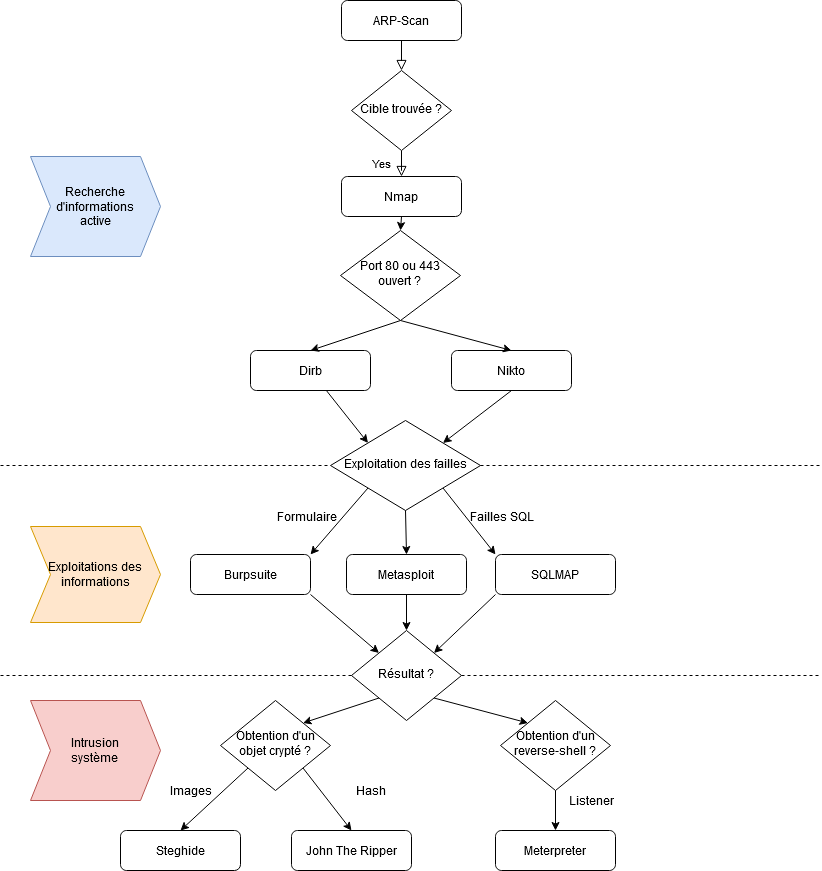
\includegraphics[width=1\textwidth]{oui/images/Chapitre1/Attackdiag.png}
  \caption{Schéma d'attaque d'un CTF}
  \label{fig:schema-ctf}
\end{figure}

Comme on a pu le comprendre, aucune attaque n'est la même et c'est en pratiquant que l'on peut comprendre pourquoi utiliser un outil plutôt qu'un autre. Cependant, avant d'utiliser ces outils, nous allons nous pencher sur notre environnement de travail.

\section{Environnement de travail}

\subsection{Kali Linux}

Kali Linux est une distribution Linux, basée sur Debian, orientée sur la sécurité informatique. Anciennement BackTrack, cette distribution a su se réinventer en devenant Kali et ainsi regrouper un nombre « incalculable » de logiciels conçus pour la sécurité et l’intrusion informatique. C’est pour cette raison que nous avons choisi de travailler sur cette distribution afin d'effectuer des CTF.

\subsection{Mise en place d'un CTF}

Pour commencer un CTF, il nous faut aller chercher une machine virtuelle attaquable. Pour cela, nous pouvons aller sur le site de Vulnhub et récupérer un fichier avec l’extension .OVA. Vulnhub est un site répertoriant des CTFs créés par la communauté. Il est donc très facile de s'exercer via ce site.\\
Ce fichier OVA contient notre machine cible que l’on pourra allumer sous Virtualbox comme vu en \textbf{figure \ref{fig:import-ova}}.

\begin{figure}[htp!]
  \centering
  \setlength\figureheight{7cm}
  \setlength\figurewidth{9cm}
  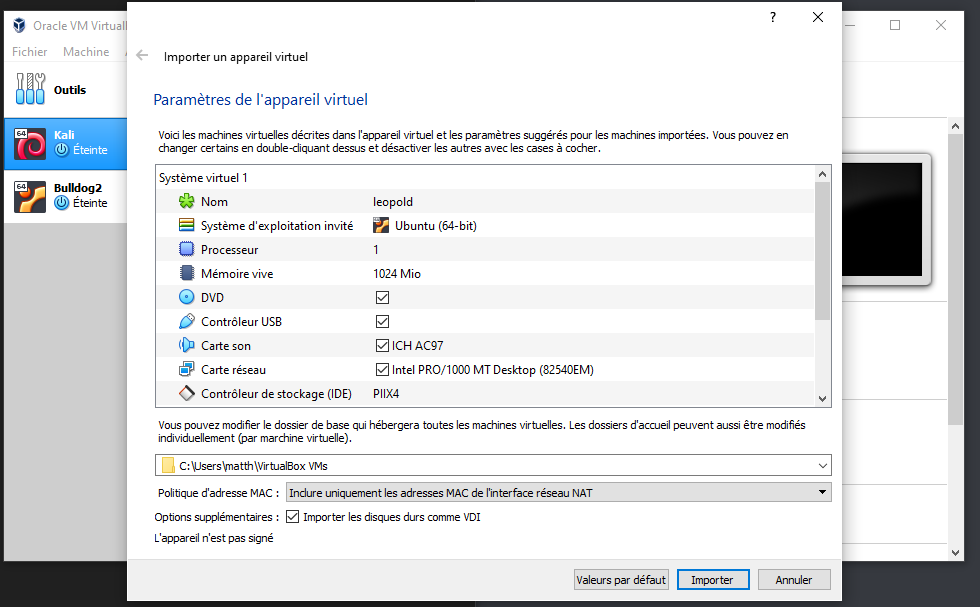
\includegraphics[width=0.77\textwidth]{oui/images/Chapitre1/importation.png}
  \caption{Imporation d'un CTF}
  \label{fig:import-ova}
\end{figure}

Après avoir réalisé cette étape, vous pourrez aller vous occuper des interfaces réseaux de votre Kali et de votre CTF afin qu'il puisse communiquer entre eux. En général, le CTF sera configuré en dhcp ce qui vous permettra d'utiliser le réseau NAT ou bien le mode Pont/Bridge. Pour rappel, le réseau NAT sous Virtualbox créé un routeur et un service DHCP entre votre ordinateur et votre machine virtuelle. Ainsi, cette dernière a accès à internet et à son propre réseau. Le mode Pont va vous permettre d'annoncer votre machine virtuelle comme machine à part entière sur votre réseau. Ainsi, la VM pourra communiquer sur votre réseau et obtenir via DHCP une adresse si le service est activé sur le réseau. Dans les deux cas, pensez à mettre votre machine attaquante et cible dans le même réseau. Une fois que cette configuration est faite, vous pourrez allumer vos machines et commencer votre attaque tout en respectant l'ordre d'attaque.
\chapter{Techniques de collecte d'informations}
\label{chap:Mini Projet}
Lors du début de chaque CTF ou de pentesting en général, il y a une phase très importante qu'il ne faut pas oublier qui est la recherche d'informations sur la machine à attaquer. Il existe 2 types de recherche d'informations :

\begin{itemize}
  \item Collecte d'informations passive
  \item Collecte d'informations active 
\end{itemize}

 Nous verrons dans un premier temps la collecte d'informations passive d'une cible puis la collecte d'informations active.

\section{Collecte d'informations passive}

La collecte d'informations passive est le moyen par lequel un attaquant peut récupérer des informations sur une entreprise ou une machine, sans entrer directement en contact avec cette dernière. En effet, ces informations sont la plupart du temps trouvable sur internet.

Par exemple, à partir de recherches sur internet, on peut trouver des adresses IP ou encore des emails ou des noms de domaines. Toutes ces informations peuvent être d'ordre publique. Une simple commande \lstinline{ping} sur un site internet permet de récupérer une adresse IP. Imaginez par exemple, une attaque contre \url{http://rt.iut-velizy.uvsq.fr/}. Il va falloir dans un premier temps déterminer quels systèmes sont utilisés par la société et quels sont les systèmes que nous pouvons attaquer. De plus, certains systèmes peuvent ne pas appartenir à la société cible et pourraient alors être considérés comme hors de portée de l'attaque.

\subsection{Whois}

Whois ("Qui est" en francais)  est un outil permettant d'interroger des bases d'informations (registres) concernant les noms de domaines et adresses IP. Les données contenues dans ces bases ne comportent aucune forme de garantie mais permettent généralement de retrouver le propriétaire d'un domaine ou d'une machine.

 Il existe plusieurs bases de données connues:

\begin{itemize}
    \item RIPE NCC (Réseaux IP Européens, whois.ripe.net) pour l'Europe
    \item APNIC (Asia Pacific Network Information Center) pour l'Asie et le Pacifique
    \item ARIN (American Registry for Internet Numbers, whois.arin.net) pour l'Amérique du Nord et l'Afrique Sub-Saharienne
    \item LACNIC (Regional Latin-American and Caribbean IP Address Registry, whois.lacnic.net) pour l'Amérique latine et les Caraïbes
    \item  INTERNIC (whois.internic.net) pour les autres parties du globe
\end{itemize}

 Il existe des sites sur internet permettant d'utiliser cet outil. Il est également présent sous Kali linux.\\

 \textbf{Utilisation de la commande whois avec Kali linux:}\\
Nous allons utiliser whois sur le site \url{uvsq.fr} dans \textbf{figure \ref{fig:whois}}.\\

\begin{figure}[htp!]
  \centering
  \setlength\figureheight{7cm}
  \setlength\figurewidth{9cm}
  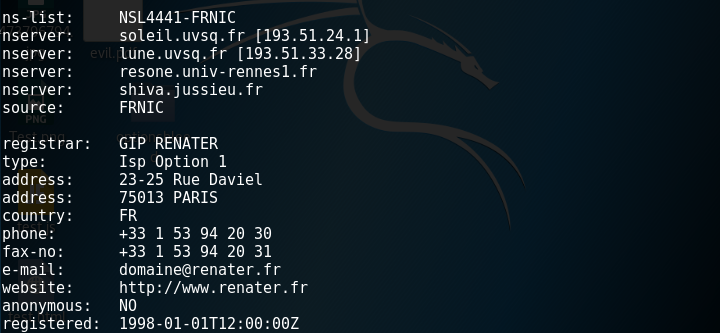
\includegraphics[width=1\textwidth]{oui/images/Whois/whois2.PNG}
  \caption{whois uvsq.fr}
  \label{fig:whois}
\end{figure}

 La commande whois nous donne des informations sur le nom de domaine \url{uvsq.fr}. On apprend ici les différents serveurs DNS qui gèrent ce domaine dans la  \textbf{figure \ref{fig:whoisdns}}.

\begin{figure}[htp!]
  \centering
  \setlength\figureheight{7cm}
  \setlength\figurewidth{9cm}
  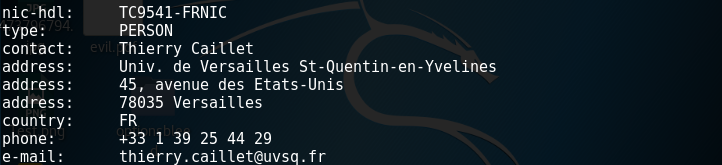
\includegraphics[width=1\textwidth]{oui/images/Whois/whois3.PNG}
  \caption{whois uvsq.fr}
  \label{fig:whoisdns}
\end{figure}

 Whois est capable de récupérer l'email de l'administateur qui gère le domaine \url{uvsq.fr}. Ces informations peuvent être plus ou moins utiles lors d'une attaque.

Il est également possible de spécifier l'adresse IP de \url{www.uvsq.fr} pour récupérer des informations relatives à l'adresse IP comme vous pouvez voir en \textbf{figure \ref{fig:whoisip}}.

\begin{figure}[b!]
  \centering
  \setlength\figureheight{7cm}
  \setlength\figurewidth{9cm}
  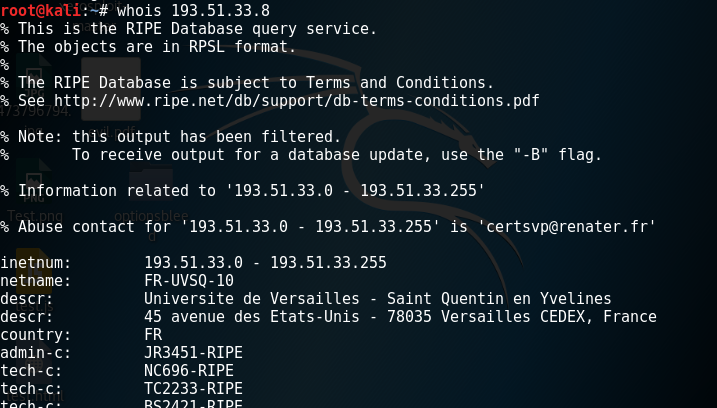
\includegraphics[width=0.9\textwidth]{oui/images/Whois/whois4.PNG}
  \caption{whois ip www.uvsq.fr}
  \label{fig:whoisip}
\end{figure}
%parler du champ inetnum et qu'on a la range d'IP pour uvsq.fr https://www.apnic.net/manage-ip/using-whois/guide/inetnum/ https://www.ripe.net/manage-ips-and-asns/db/support/documentation/ripe-database-documentation/rpsl-object-types/4-2-descriptions-of-primary-objects/4-2-4-description-of-the-inetnum-object
 --- Le champ \textbf{inetnum} correspond à une plage d'adresse IP détenue par le domaine en question. Par exemple, pour le domaine \url{uvsq.fr} sa plage d'IP sera comprise entre \textbf{193.51.33.0} et \textbf{193.51.33.255}.\\

Un simple script en python permet de vérifer cela et d'obtenir un résultat visible en \textbf{figure \ref{fig:resultatprogpy}}.  (Script en annexe \ref{fig:nslookup})

\begin{figure}[b!]
  \centering
  \setlength\figureheight{7cm}
  \setlength\figurewidth{9cm}
  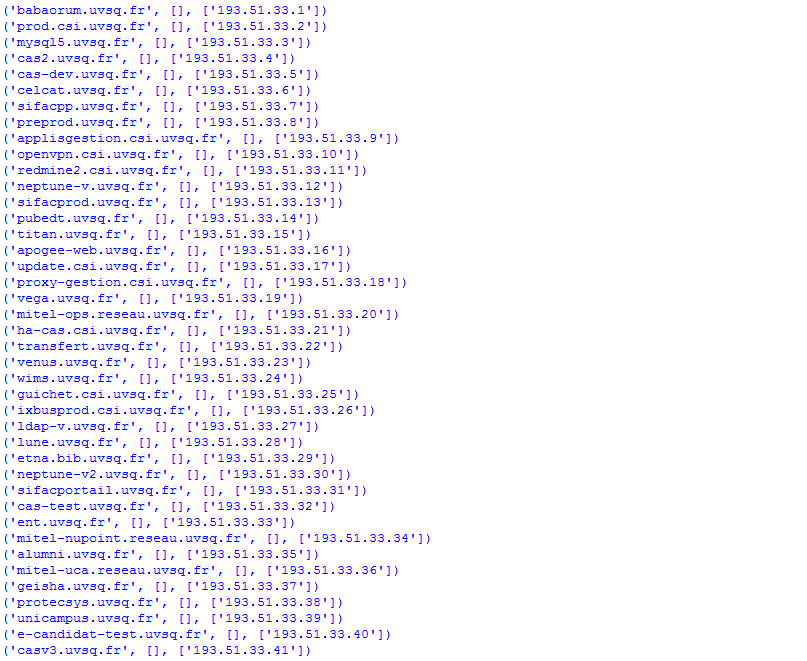
\includegraphics[width=0.8\textwidth]{oui/images/Whois/script-python.PNG}
  \caption{Résolution DNS pour la plage d'ip de uvsq.com}
  \label{fig:resultatprogpy}
\end{figure}

 On constate à travers cette capture que les IP de la plage pointent vers le nom de domaine \url{uvsq.fr}. Cela peut être très utile pour cibler des services à attaquer avec leur IP public. Par exemple, l'IP \textbf{193.51.33.3} semble correspondre à un potentiel serveur mysql à en croire son nom. On remarque également que l'autorité de \textbf{uvsq.com} a créé un alias de l'enregistrement \textbf{www} vers \textbf{preprod.uvsq.com}, puisque ces noms ont les même IP et qu'ils redirigent tous deux vers le site internet de l'uvsq.\\

 --- Le champ \textbf{netname} correspond au nom donné à une plage d'adresses IP. Un nom de réseau est composé de lettres, de chiffres, du caractère de soulignement et du trait d'union. Le premier caractère d'un nom doit être une lettre, et le dernier caractère d'un nom doit être une lettre ou un chiffre.\\

\subsection{Nslookup}

L'outil Nslookup est un outil implanté sur beaucoup de systèmes d'exploitation (OS) tel que Windows ou Linux. Cet outil permet de faire des résolutions DNS à partir d'un nom de domaine. En effet, cela est très pratique lorsqu'on veut récupérer une IP à partir d'un nom tel que \textbf{www.uvsq.fr}.\\

 \textbf{Fonctionnement requête DNS}\\

Nous allons ici présenter le bref fonctionnement d'une requête DNS puisque cette partie a déjà été expliqué dans d'autres modules auparavant. En premier lieu, le DNS permet d'associer un nom à une IP ce qui est très utile pour l'être humain.\\

 Le protocole DNS est un protocole UDP avec comme numéro de port 53. Le DNS est un modèle réparti hiérarchisé, sa mise en œuvre requiert plusieurs serveurs qui prennent en charge individuellement la traduction de parties complémentaires de l’espace des noms afin de rendre plus souple le traitement des sollicitations. Ces parties appelées "zones" sont en fait des domaines de noms dont l’administration est définie et attribuée à un ou plusieurs serveurs.

 La \textbf{figure \ref{fig:repartitiondns}} nous présente un schéma de la répartition des zones DNS.

\begin{figure}[htp!]
  \centering
  \setlength\figureheight{7cm}
  \setlength\figurewidth{9cm}
  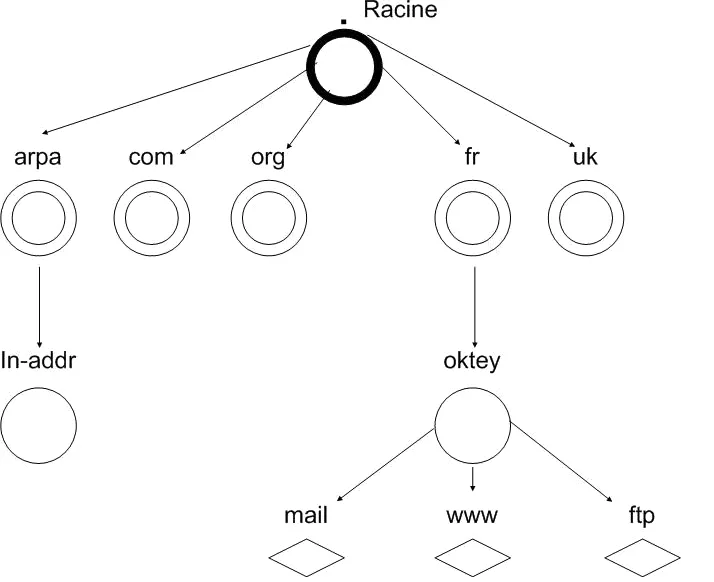
\includegraphics[width=0.5\textwidth]{oui/images/Nslookup/dns.png}
  \caption{Répartition des zones DNS}
  \label{fig:repartitiondns}
\end{figure}

 Le domaine Racine est géré par les 13 serveurs DNS nommés \lstinline{<x>.root-servers.net}, où \lstinline{<x>} est une lettre comprise entre ‘a’ à ‘m’. Ces serveurs racines sont gérés par des organisations différentes nommées par l’ICANN. Les domaines enfants sont dits les domaines de premier niveau ou TLD (Top Level Domain). On y retrouve le domaine .com, .fr etc...\\

\newpage

Expliquons maintenant ce qu'il se passe lorsqu'un client effectue une requête DNS.

Il existe deux types de requête DNS. Les requêtes itératives, et récursives. Nous ne présenterons ici que les requêtes récursives, comme illustré sur la \textbf{figure \ref{fig:dns2}}.

\begin{figure}[t]
  \centering
  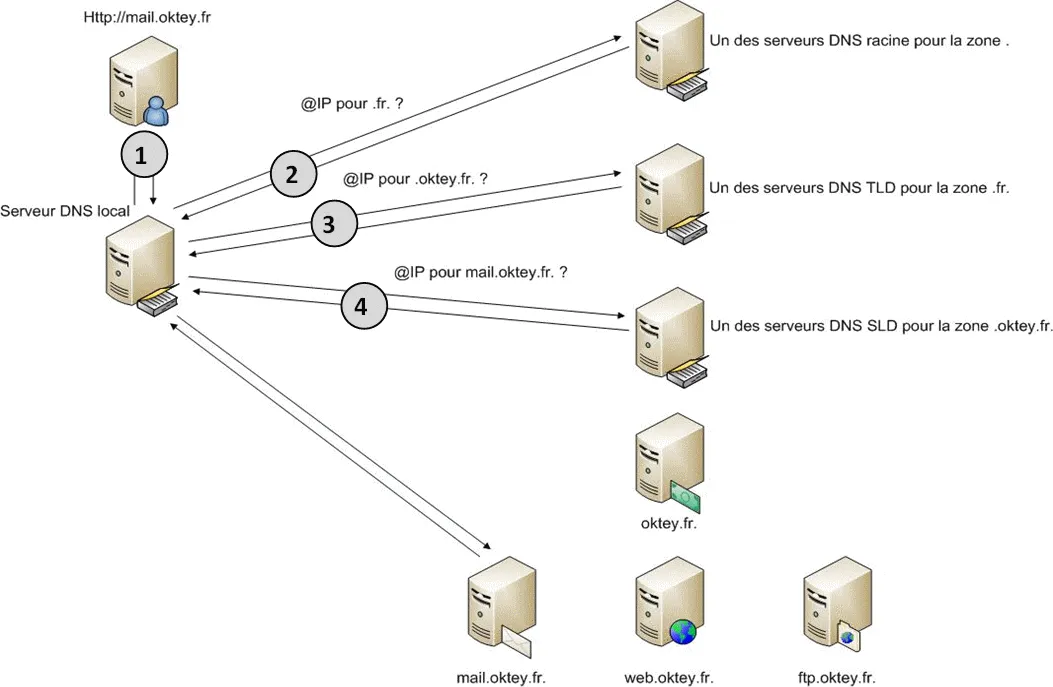
\includegraphics[width=0.6\textwidth]{oui/images/Nslookup/dns2.png}
  \caption{Schéma d'une requête DNS récursive}
  \label{fig:dns2}
\end{figure}

\begin{enumerate}
    \item Le client effectue une requête DNS à son serveur DNS local.
    \item Le serveur DNS contacte le serveur racine pour récupérer l'ip du serveur TLD de la zone fr.
    \item Le DNS local contacte le TLD de la zone fr pour récupérer l'ip du sous domaine oktey.
    \item Ce dernier contacte le serveur qui fait autorité sur la zone oktey.fr pour récupérer l'ip associé à l'enregistrement mx de mail.okley.fr.
\end{enumerate}

 On constate qu'avec l'utilisation des requête récursives, c'est le serveur DNS local qui s'occupe de faire toutes les requêtes.\\
 Avec l'outil \textbf{Nslookup}, il est également possible d'effectuer une résolution inverse. En effet, cette dernière permet de récupérer le nom associé à une adresse IP. Pour ce faire, on utilise le domaine \textbf{in-addr.arpa} (RFC 1035) pour retrouver le nom associé.

 La technique de résolution inverse a été utilisée dans la figure 2.4. En effet, à partir de la plage d'IP récupéré avec l'outil \textbf{whois}, on peut effectuer des résolutions inverses pour tenter de récupérer le nom derrière ces IP. Ainsi, cela peut nous indiquer un service qui serait hébergé par cette IP. A partir de là, il sera plus facile d'orienter nos recherches pour continuer l'attaque.


\subsection{Maltego}

Maltego est un outil open source intélligent permettant la recherche d'informations précises sur une personne ou une entreprise. On appel ce genre d'outil un footprinting (reconnaissance passive). Maltego permet l'automtisation des tâches de recherches. Ainsi, avec ces informations, Maltego les représentent sous forme d'un graphique détaillé.\\

\begin{figure}[htp!]
  \centering
  \setlength\figureheight{7cm}
  \setlength\figurewidth{9cm}
  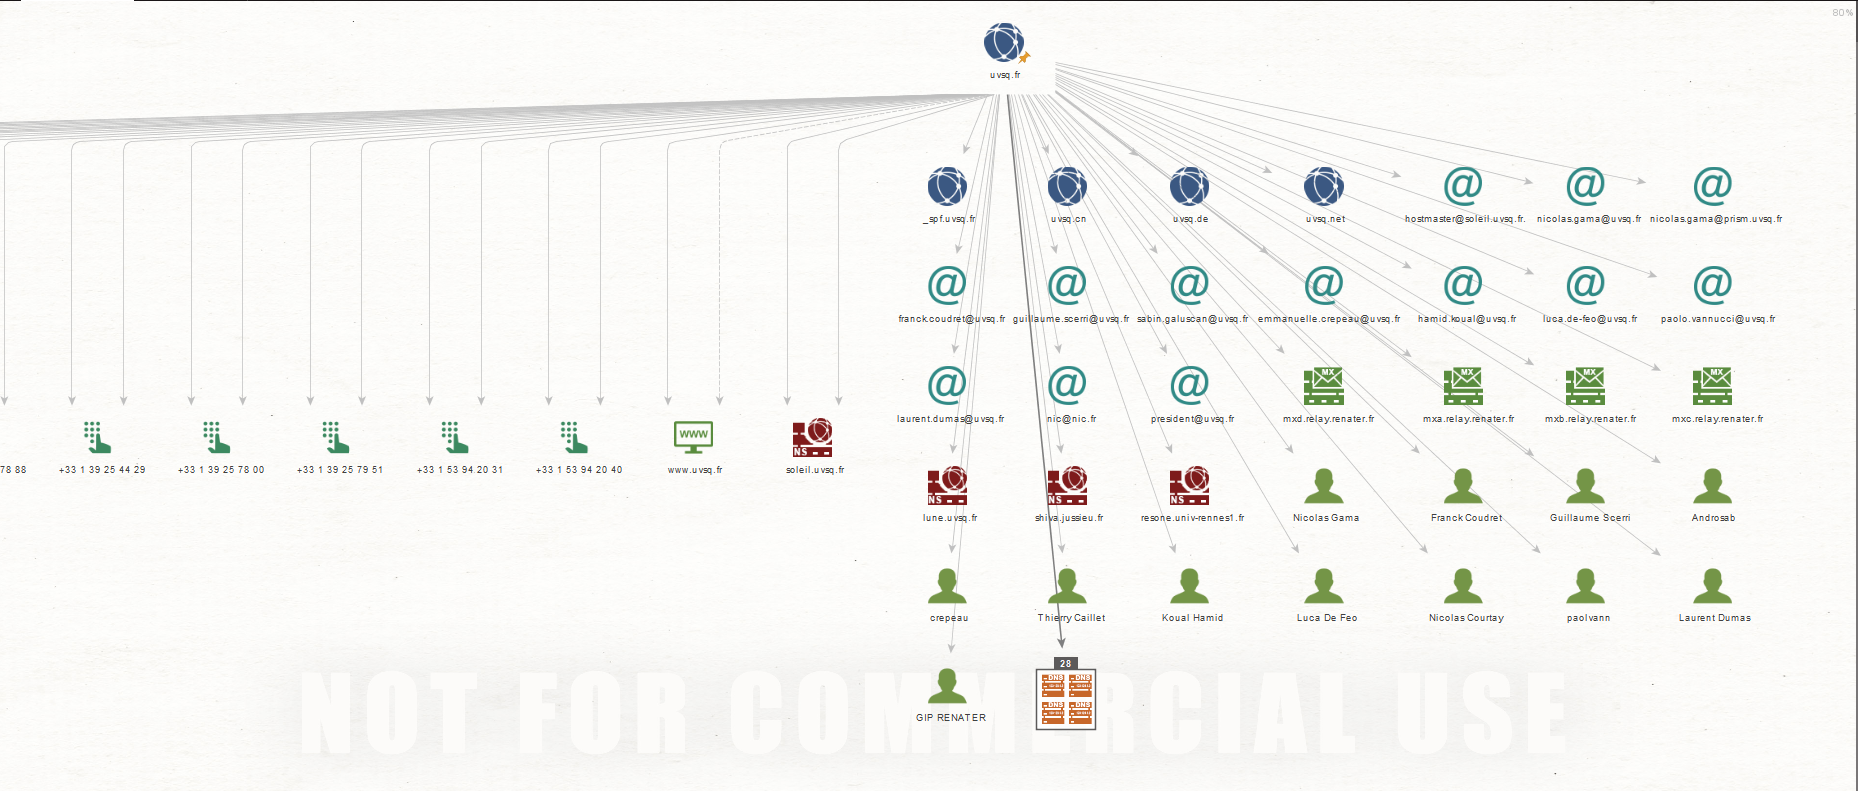
\includegraphics[width=1\textwidth]{oui/images/maltego/uvsq2.PNG}
  \caption{Présentation graphique de maltego}
  \label{fig:graphmaltego}
\end{figure}

\newpage
Dans la \textbf{figure \ref{fig:graphmaltego}}, on peut voir l'utilisation de Maltego sur le domaine \textbf{uvsq.com}. On peut donc récupérer des adresses mails, des numéros de téléphone, des noms de personnes ainsi que les sous domaines DNS associés à \textbf{uvsq.com}. Il est également possible de récupérer des adresses IP ainsi que le numéro d'AS sur lequel le site est hébergé.\\

Pour fonctionner, Maltego travaille à partir de bases de données ainsi que de recherches faites sur le web. En somme, cela évite à l'utilisateur de faire de longues recherches pour trouver une information sur une personne ou un site. Cela peut être extrêmement utile lors de la collecte d'informations sur une entreprise. En effet, avec les informations que nous pouvons récupérer, il serait possible de cibler plus facilement les attaques ou même de faire du phishing avec les adresses emails obtenues.
%

\newpage
\section{Collecte d'informations active}

La collecte d'informations active va consister à reccueillir des informations en effectuant des requêtes sur le réseau et/ou machine cible. Cette étape va donc nous permettre de récupérer des informations telles que l'IP, l'adresse MAC, les ports ouverts, etc... Sans cette phase, une attaque serait impossible. C'est pourquoi il est important de penser à marquer dans un fichier texte l'ensemble des informations obtenues au cours de cette recherche. Nous allons dans cette partie vous présenter les outils adéquats et leur fonctionnement afin que vous puissiez obtenir facilement les données que nous pourrons exploiter par la suite. Nous verrons les outils suivants :

\begin{itemize}
    \item Arp-scan en tant que scanneur de machines
    \item Nmap en tant que scanneur de ports
    \item Dirb / Dirbuster en tant que scanneur de répertoire Web
    \item Nikto en tant que scanneur de vulnérabilités
\end{itemize}

\subsection{Arp-scan}

Arp-scan est un utilitaire qui permet  d’obtenir les adresses IP d’un réseau via la couche 2 du modèle OSI . Le modèle OSI est une norme d’exemple pour tous les types de transmissions réseaux. Ce modèle peut être vu comme en \textbf{figure \ref{fig:osi}}.
%Image modèle OSI
\begin{figure}[htp!]
  \centering
  \setlength\figureheight{7cm}
  \setlength\figurewidth{9cm}
  \includegraphics[width=0.4\textwidth]{oui/images/Arpscan/modeleOSI.PNG}
  \caption{Schéma du modèle OSI}
  \label{fig:osi}
\end{figure}

La couche 2 est la couche de liaison de données. Cette dernière correspond à l’adressage physique des machines, soit l’adresse MAC. L’adresse MAC est l’adresse unique d’une interface réseau d’un équipement. Cette adresse est codée en hexadécimal en 6 octets.\\

 \textbf{Fonctionnement d'Arp-scan}\\

Cet outil va envoyer une requête ARP en broadcast sur le réseau et afficher l’IP, l'adresse MAC ainsi que, si possible, l'origine de chaque hôte. Si un hôte ne répond pas, le paquet ARP sera envoyé à nouveau. Le nombre maximum de tentatives peut être modifié avec l'option --retry. Cependant, si l'on réduit le nombre de tentatives, alors cela réduira le temps du scan mais engendrera le risque de perdre certains résultats en raison de la perte de paquets.
Comme vous pouvez le voir sur la \textbf{figure \ref{fig:arpscanwireshark}}, la capture Wireshark effectuée après un "arp-scan" se présente de la même manière qu’une requête ARP.

%Image Wireshark arp broadcast
\begin{figure}[htp!]
  \centering
  \setlength\figureheight{7cm}
  \setlength\figurewidth{9cm}
  
\includegraphics[width=1\textwidth]{oui/images/Arpscan/wireshark.PNG}
  \caption{Capture Wireshark}
  \label{fig:arpscanwireshark}
\end{figure}

Le protocole ARP est un protocole de niveau 2 (couche de liaison de données) qui est utilisé pour déterminer l'adresse MAC (couche 2) d'un hôte distant à partir de son adresse IP (couche 3). Le protocole ARP a été conçu pour fonctionner avec n'importe quel format d'adresse de couche 2 et de couche 3, mais l'utilisation la plus courante est de cartographier un réseau.
Cependant, cet outil ne peut être utilisé que sur des réseaux LAN car les requêtes ARP ne peuvent pas être routées dans le cas d’un scan de réseau Local.
Ce protocole utilise des adresses IP, mais il n'est pas basé sur IP. Ainsi, Arp-scan peut être utilisé sur une interface qui n'est pas configurée pour IP. La \textbf{figure \ref{fig:arpscanl}} présente l'utilisation la plus commune de cet outil.

\begin{figure}[htp!]
  \centering
  \setlength\figureheight{7cm}
  \setlength\figurewidth{9cm}
  \includegraphics[width=0.9\textwidth]{oui/images/Arpscan/unknown.png}
  \caption{Arp-scan  - -localnet}
  \label{fig:arpscanl}
\end{figure}

Une fois l'IP cible récupérée, nous allons pouvoir analyser ses ports avec Nmap.

\subsection{Nmap}

Nmap est un utilitaire permettant de scanner les ports ouverts d’une machine ou d’un ensemble de machines présentes dans un même réseau. Les ports (logiciels) d'une machine permettent de distinguer les différents programmes qui écoutent et transmettent des informations sur cette machine. En effet, chaque programme ou service se verra atribuer un numéro de port qui servira à identifer le processus associé. En trouvant ces ports, Nmap se rend comme l’élément essentiel d’une attaque réseau. En effet, sans cette analyse, nous serions incapable de trouver un chemin d’attaque à moins d’avoir une chance inouïe. C’est pourquoi nous allons utiliser cet utilitaire pour résoudre nos CTFs.\\

 \textbf{Fonctionnement de Nmap}\\

Pour comprendre comment fonctionne Nmap, il va falloir revoir les bases du protocole TCP grâce à la \textbf{figure \ref{fig:3way}}.


\newpage

\begin{figure}[htp!]
  \centering
  \setlength\figureheight{7cm}
  \setlength\figurewidth{9cm}
  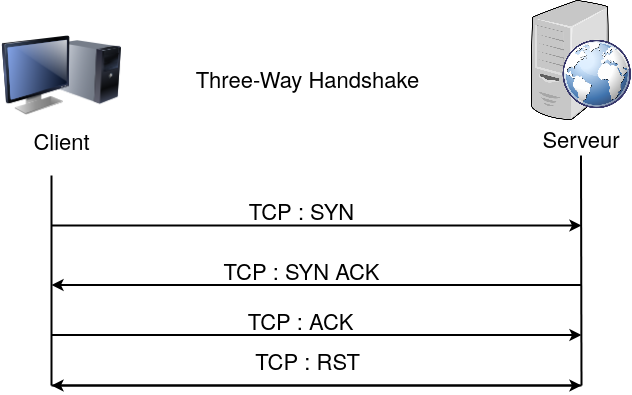
\includegraphics[width=0.8\textwidth]{oui/images/nmap/3way.png}
  \caption{Three-way Handshake}
  \label{fig:3way}
\end{figure}

Le protocole TCP de TCP-IP est situé au niveau de la couche Transport du modèle OSI (couche 4). Il va nous permettre d'établir une connexion fiable et sans pertes. Dans un premier temps, TCP va établir la connexion via le Three-way Handshake qui sont :

\begin{itemize}
    \item SYN
    \item SYN ACK
    \item ACK
\end{itemize}

A la suite de cette étape, le protocole de plus haut niveau faisant les requêtes pourra émettre et sera suivi dans un ACK TCP pour s'assurer de l'intégrité de la trame comme on peut le voir sur la \textbf{figure \ref{fig:acktcp}}.

\begin{figure}[htp!]
  \centering
  \setlength\figureheight{7cm}
  \setlength\figurewidth{9cm}
  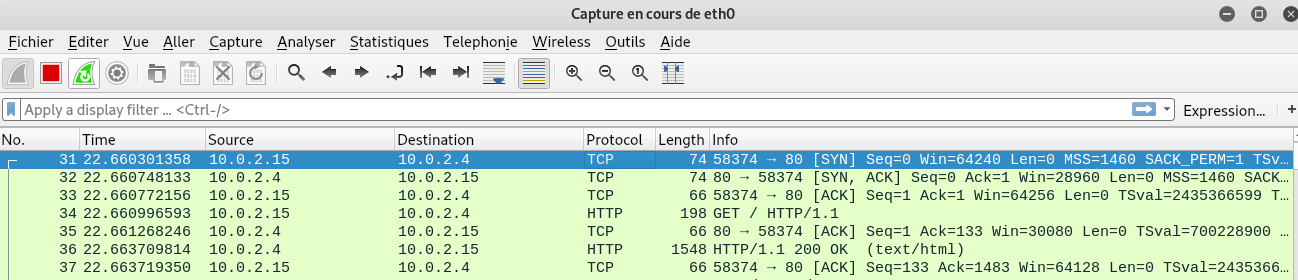
\includegraphics[width=1\textwidth]{oui/Ancien/imangeancien/Nikto/wireshark1.PNG}
  \caption{ACK TCP}
  \label{fig:acktcp}
\end{figure}

Sur l'exemple ci-dessus, on peut voir dans la section "Info" de Wireshark que les ports sont indiqués. On comprend alors que TCP ne cible pas une IP mais un socket. Un socket est l'ensemble de l'adresse IP et du port utilisé. Il est souvent représenté sous la forme suivante : \verb+192.168.1.200:80+. C'est donc en faisant varier le port du socket que Nmap pourra détecter si un port est ouvert ou non. Ainsi, si Nmap reçoit une réponse que de la machine cible à la suite d'un SYN TCP, cela voudra dire que le port est ouvert.\\
Maintenant que nous avons compris comment Nmap détecte si un port est ouvert ou non, nous allons nous intéresser à la détection du service associer à ce port. En effet, Nmap peut fournir le nom et même la version d'un service déployé sur un port d'une machine cible.\\

 Pour cela, l'outil se base sur deux fichiers qu'il utilise comme dictionnaire. Ces deux documents se situent dans son dossier d'éxécution et sur internet :

\begin{itemize}
    \item \textbf{nmap-services: https://svn.nmap.org/nmap/nmap-services}
    \item \textbf{nmap-services-probes: https://svn.nmap.org/nmap/nmap-service-probes}
\end{itemize}

 Le fichier nmap-services contient une association de nom de service en fonction du port. En effet, il existe trois catégories de ports :

\begin{itemize}
    \item \textbf{1-1023 : Well-known ports}
    \item \textbf{1024-49151 : Registered ports}
    \item \textbf{49152-65535 : Dynamic ports}
\end{itemize}

 Les "Well-kown ports" sont des ports attitrés à des service par l'IANA (Internet Assigned Numbers Authority). Ces services sont les plus connus du monde des réseaux et doivent être éxécutés en tant qu'administrateur. Les "Registered ports" sont eux aussi attribués par l'IANA mais ne nécessitent pas d'une éxecution en tant qu'administrateur. Les "Dynamic ports" ou ports dits "éphémères", comme le nom l'indique, sont distribués de manière dynamique par le système d'exploitation afin de pouvoir rentrer en contact avec un service. C'est donc en fontion de ce recensement que Nmap met à jour sa liste nmap-services. La question la plus légitime à la suite de cette explication est la suivante :\\
"Comment Nmap peut récupérer le nom d'un service déployé sur un port n'ayant pas été répertorié ?"\\
Nmap vous répondra en fonction de votre requête. En effet, si vous n'effectuez qu'un simple scan, l'outil ne va s'appuyer que sur nmap-services pour détecter le service. Cependant, si vous vous voulez avoir de plus amples informations sur le port, il vous faudra effectuer un scan de version. Ce scan se base sur le fichier "nmap-service-probes". Ce dernier contient des requêtes à effectuer en fonction des ports ouverts et des expressions régulières à tester avec la réponse du services. Si le test est positif, Nmap pourra afficher les informations présentes à la suite de l'expression régulière. Ce type de scan est donc beaucoup plus précis. La \textbf{figure \ref{fig:fonctionnementnmap}} représente donc le fonctionnement de base de Nmap.

\begin{figure}[htp!]
  \centering
  \setlength\figureheight{7cm}
  \setlength\figurewidth{9cm}
  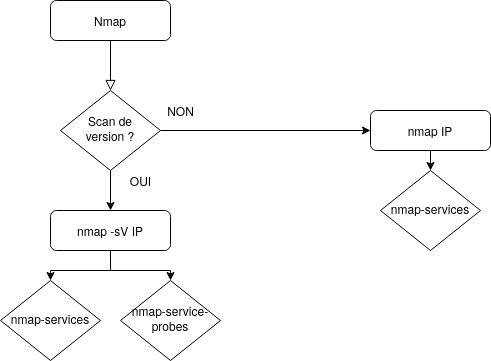
\includegraphics[width=0.9\textwidth]{oui/images/nmap/basenmapdiag.png}
  \caption{Schéma fonctionnement Nmap}
  \label{fig:fonctionnementnmap}
\end{figure}

Nous allons voir maintenant comment appliquer ce fonctionnement à un CTF.

 \textbf{Application de Nmap}\\

Dans cette partie, nous allons voir comment utiliser Nmap en ligne de commandes (CLI) en fonction des informations que l'on souhaite récupérer.\\

 \textbf{Mode basique}\\

Si vous souhaitez ne faire qu'un scan rapide sans option, la \textbf{figure \ref{fig:scanbasique}} présente la commande à effectuer.

\begin{figure}[htp!]
  \centering
  \setlength\figureheight{7cm}
  \setlength\figurewidth{9cm}
  \includegraphics[width=0.7\textwidth]{oui/Ancien/imangeancien/Nmap/justeip.PNG}
  \caption{Scan basique}
  \label{fig:scanbasique}
\end{figure}

Comme on peut le voir ci-dessus, le résultat de ce scan simple nous permet de savoir que le port 80 est ouvert et que le sevice associé est HTTP. Si on observe un peu plus cette capture d'écran, on peut voir que Nmap a résolu via DNS le nom de notre cible qui est ici bulldog2-1.\\
Du côté de Wireshark, nous pouvons observer, en \textbf{figure \ref{fig:wirebasique}}, sa technique de détection de port que l'on nomme "la semi-ouverture de ports".

\begin{figure}[htp!]
  \centering
  \setlength\figureheight{7cm}
  \setlength\figurewidth{9cm}
  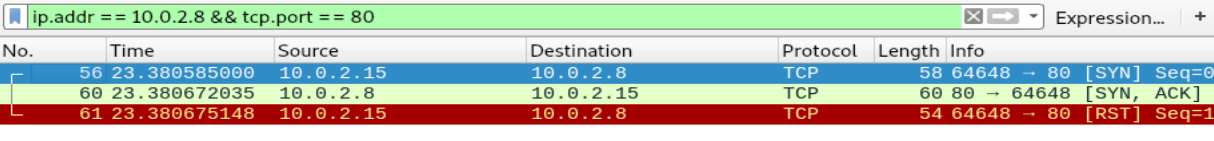
\includegraphics[width=1\textwidth]{oui/images/nmap/Wirebasique.PNG}
  \caption{Wireshark d'un scan de port 80}
  \label{fig:wirebasique}
\end{figure}

Dans le cas ci-dessus, l'attaquant est en 10.0.2.15 et la cible en 10.0.2.8. On se rend compte Nmap ne complète pas le Three-way Handshake et coupe brutalement la connexion via un RST TCP.
Ce scan est très rapide mais manque d'informations et est très visible sur le réseau... Il n'est pas forcément à privilégier.\\

 \textbf{Scan de version}\\

Si vous souhaitez obtenir des informations concerant le serveur de déployement du service afin de trouver des failles associées, il vous faudra utiliser l'option -sV de Nmap visualisable en \textbf{figure \ref{fig:sv}}.

\begin{figure}[htp!]
  \centering
  \setlength\figureheight{7cm}
  \setlength\figurewidth{9cm}
  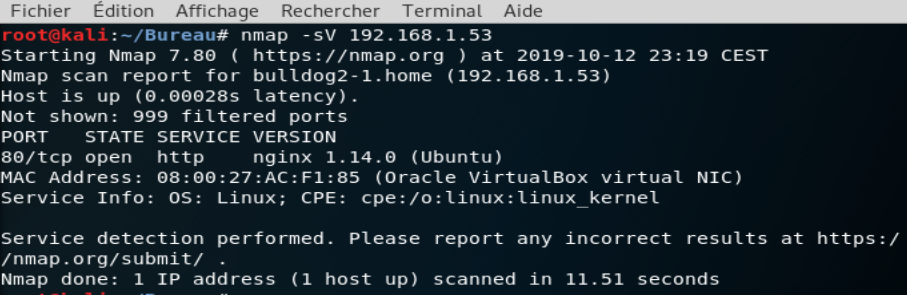
\includegraphics[width=0.8\textwidth]{oui/Ancien/imangeancien/Nmap/-sV.PNG}
  \caption{Scan de version}
  \label{fig:sv}
\end{figure}

\newpage
Ce scan affiche une nouvelle colonne qui contient les informations du service. Regardons ce qu'il se passe au niveau de Wireshark en \textbf{figure \ref{fig:svwire}}.

\begin{figure}[htp!]
  \centering
  \setlength\figureheight{7cm}
  \setlength\figurewidth{9cm}
  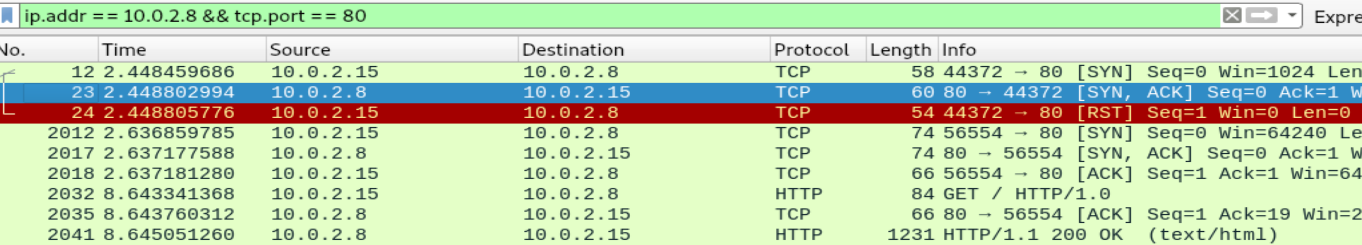
\includegraphics[width=1\textwidth]{oui/images/nmap/Wireversion.PNG}
  \caption{Obtention d'informations de version sous Wireshark}
  \label{fig:svwire}
\end{figure}

Dans un premier temps, nous retrouvons bien la demi-ouverture de port puis Nmap effectue le 3-way Handshake afin de se connecter au service qui est ici HTTP. Il va ensuite aller chercher dans son dictionnaire nmap-service-probes les requêtes à effectuer afin d'obtenir des informations. Dans notre cas, il va commencer par effectuer un GET et obtenir une réponse dans le HTTP/1.1 200 OK. Cela signifie que la page existe et que son retour est positif. Par exemple, si nous avions ouvert la réponse envoyée par la cible, nous aurions vu tout le contenu HTML de la page. Cette réponse est donc comparée à des expressions régulières présentes dans le fichier nmap-service-probes. Ce type de scan est donc plus approprié afin de trouver des failles. Cependant, il existe un moyen beaucoup plus complexe et complet qui est le scan via script.\\

 \textbf{Scan par script}\\

Dans le but d'obtenir des informations très précises, Nmap peut aussi s'éxecuter avec l'aide de scripts. Cette méthode s'appelle "Nmap Scripting Engine" ou NSE et s'appuie donc sur les mécanismes de Nmap et sur la légèreté des scripts Lua. Le langage Lua est très présent dans le monde du réseau comme par exemple dans Wireshark, dans les routeurs Cisco et d'autres. Nmap contient dans son répertoire près de 601 scripts regroupés sous 139 catégories. Il est donc tout à fait possible de créer un script et de l'excécuter avec Nmap. Cependant, nous allons nous baser sur un script déjà fait et qui exécute plusieurs scripts de différentes catégories afin d'obtenir des réponses précises et variées. Ce script est l'option par défault choisi par Nmap lors de la présence de l'argument -sC comme indiqué sur la \textbf{figure \ref{fig:nse}}.\\

\begin{figure}[t!]
  \centering
  \setlength\figureheight{7cm}
  \setlength\figurewidth{9cm}
  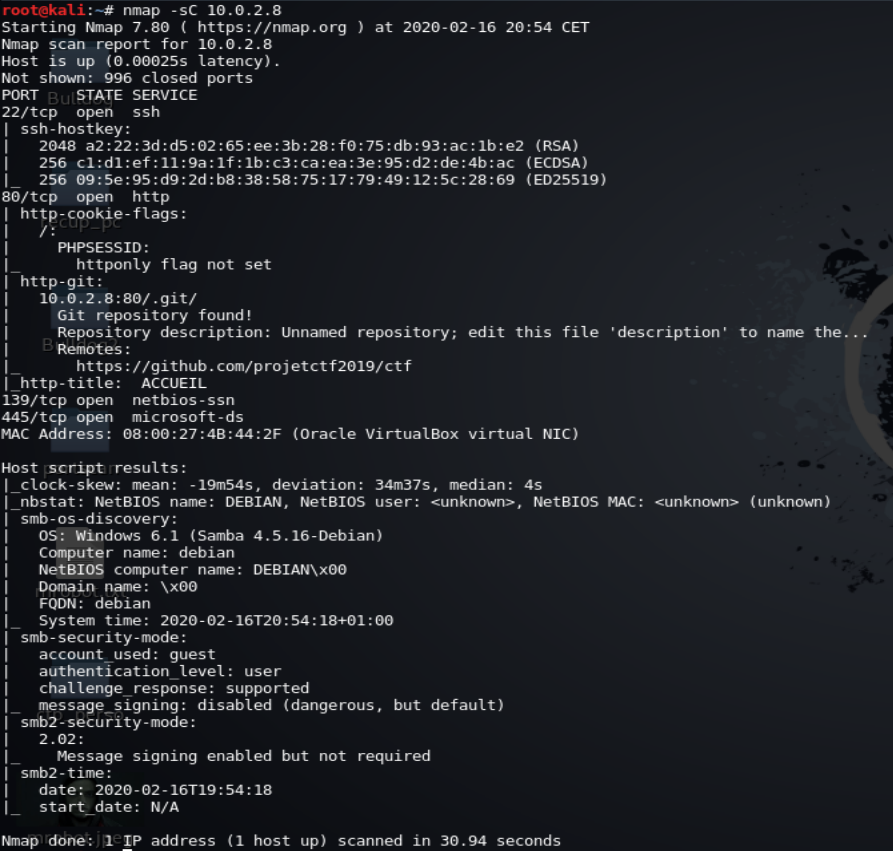
\includegraphics[width=0.8\textwidth]{oui/images/nmap/scriptscan.PNG}
  \caption{NSE par défaut}
  \label{fig:nse}
\end{figure}

On s'aperçoit que la quantité d'informations est très importante. Ce type de scan est le moyen ultime pour récupérer le plus d'informations possible. Il sera donc à privilégier lors d'un CTF.\\

\newpage

 \textbf{Devenir invisible}\\

Avoir des informations, c'est bien, mais les récupérer en étant discret, c'est mieux. En effet, si la machine cible n'était pas un CTF mais un cas réel d'attaque, il nous faudrait apprendre à ne pas être détécté. Il existe de multiples moyens que nous allons voir ici. Dans un premier temps, il faut savoir que Nmap utilise l'option -sS par défaut. Ce mode permet à Nmap de ne réaliser qu'une demi-ouverture de porte. Cet option est essentielle afin de ne pas être détecté trop vite. Ensuite, nous avons la possiblité d'usurper notre identité via un spoof MAC et IP comme on peut le voir sur la \textbf{figure \ref{fig:spoofip}}\\

\begin{figure}[]
  \centering
  \setlength\figureheight{7cm}
  \setlength\figurewidth{9cm}
  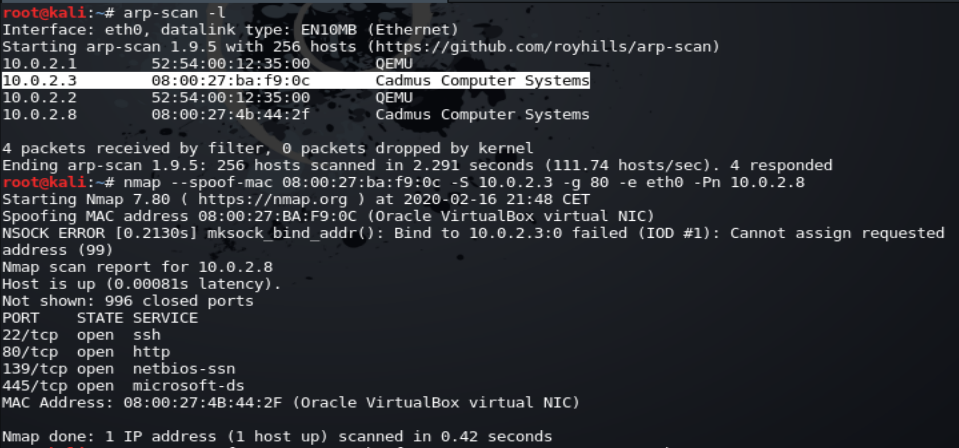
\includegraphics[width=1\textwidth]{oui/images/nmap/spoof.PNG}
  \caption{Spoof MAC et IP}
  \label{fig:spoofip}
\end{figure}

Cette méthode consiste à se faire passer pour quelqu'un du réseau via son adresse MAC et IP. L'option -g permet d'indiquer vers quel port de la machine usurpée Nmap va rediriger les échanges. L'option -e indique sur quelle interface réseau la machine attaquante va recevoir les informations telles que l'attaque "Man in the middle". Enfin, l'option -Pn n'est pas obligatoire mais elele est conseillée par Nmap en cas d'usurpation d'identité. En effet, cette option permet de bloquer le protocole ICMP et ainsi de ne pas être découvert.\\
%ça te va ?
La seconde méthode permet d'être moins visible vis à vis d'un firewall et de cibler les ports les plus connus tout en réduisant le temps de scan de ports. En moyenne, la durée d'un scan par défaut de Nmap est de 1 seconde. Il est possible de faire varier le temps d'un scan afin de faire baisser le nombre d'ouverture de ports par seconde en utilisant l'argument -Tx. Il est à notifier que le x est comprit entre 0 et 5 et que plus le x sera grand, plus le scan sera agressif. \\

\vspace{0.1cm}

Cependant, si on recherche à être discret et que l'on choisit un x valant 1 ou 0, le scan risque d'être très long... En effet, l'option -T1 réalise le scan en 30 secondes minimum tandis que le -T0 le réalise en 10 minutes ! La solution la plus adaptée est donc de cibler des ports stratégiques avec l'argument -p comme indiqué dans la \textbf{figure \ref{fig:port}}.\\



\begin{figure}[]
  \centering
  \setlength\figureheight{7cm}
  \setlength\figurewidth{9cm}
  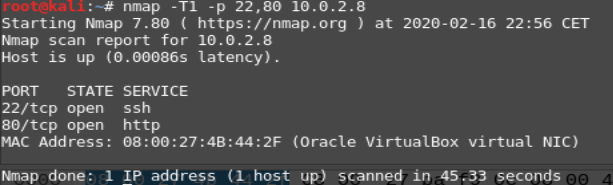
\includegraphics[width=1\textwidth]{oui/images/nmap/t1.PNG}
  \caption{Ciblage des ports}
  \label{fig:port}
\end{figure}

Nous avons donc compris dans cette partie que l'outil Nmap est essentiel lors d'une attaque et qu'il comporte énormément de fonctionnalités.

\section{Nikto}

\subsection{Présentation}
Nikto est un outil écrit en Perl permettant le scan de vulnérabiltés sur un serveur Web. Il permet de tester la sécurité de la configuration d'un serveur web (les options HTTP, les index, les potentielles failles XSS, injections SQL etc…).\\
Avant de montrer ce que peut réaliser Nikto, nous pouvons dans un premier temps revoir comment fonctionne une requête Web. Parmis les ports réservés, les serveurs Web utilise le port 80 pour HTTP et le port 443 pour l'HTTPS. Pour comprendre le fonctionnement, nous allons analyser un échange entre un client et un serveur sur la \textbf{figure \ref{fig:webdiag}}.\\



\begin{figure}[t]
  \centering
  \setlength\figureheight{7cm}
  \setlength\figurewidth{9cm}
  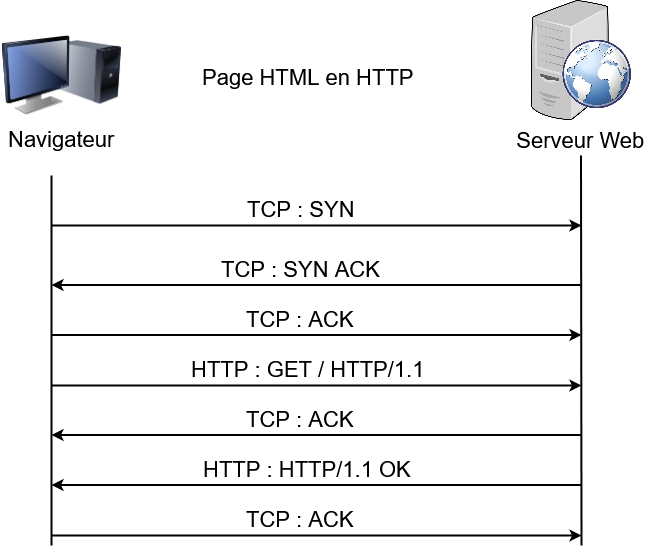
\includegraphics[width=0.7\textwidth]{oui/Ancien/imangeancien/Nikto/wEBDiagram.png}
  \caption{Échange entre un navigateur et un serveur Web}
  \label{fig:webdiag}
\end{figure}


Comme on peut le voir, le schéma sur la \textbf{figure \ref{fig:webdiag}}. ainsi que la capture wireshark en \textbf{figure \ref{fig:niktowire}} montrent l'échange minimal entre un navigateur et un serveur Web afin d'obtenir une page HTML via HTTP. Une page Web utilse le protocole TCP pour transmettre les paquets. En effet, lorsque nous chargeons une page Web, nous la voulons complète et sans erreurs. C'est pourquoi le protocole TCP existe. Au début de chaque trame TCP, il ya une synchronisation de la connexion avec le "3 way handshakes". Passons maintenant à la couche applicative : les envois HTTP sont directement émis par le navigateur et par le serveur Web. Ici, c'est notre navigateur qui fait une requête GET au serveur pour obtenir l'ensemble de la page Web voulue. Il existe plusieurs types de requêtes Web (GET, POST, HEAD, ...) mais seul le GET va nous intéresser car il est le plus utilisé. 

\begin{figure}[htp!]
  \centering
  \setlength\figureheight{7cm}
  \setlength\figurewidth{9cm}
  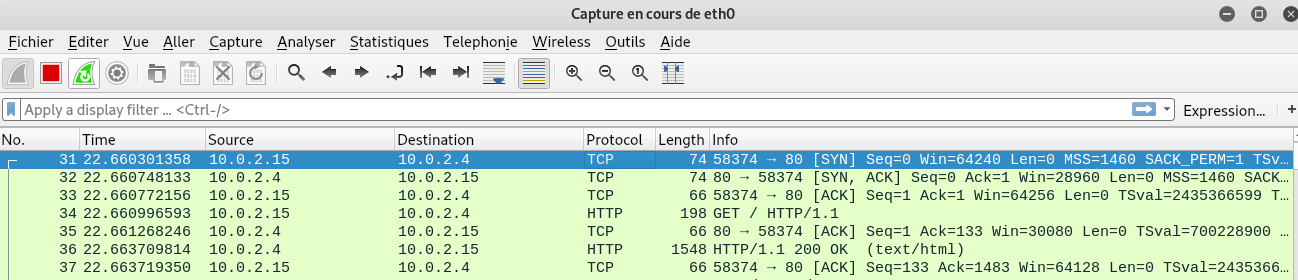
\includegraphics[width=0.7\textwidth]{oui/Ancien/imangeancien/Nikto/wireshark1.PNG}
  \caption{Capture Wireshark d'un scan nikto}
  \label{fig:niktowire}
\end{figure}


 Lors du scan, Nikto est capable de :\\
\textbf{- Vérifier} si la version du serveur est obsolète ainsi que les logiciels et     modules qui sont utilisés par ce dernier. \\   
\textbf{- Scanner} les répertoires, qui peuvent contenir des informations sensibles.\\
\textbf{- Tester} près de 6000 fichiers potentiellement vulnérables.\\
De plus, Nikto supporte les connexions SSL.


\newpage

\subsection{Utilisation de Nikto}

 Pour lancer un simple scan, il suffit de taper la commande :

\begin{figure}[htp!]
  \centering
  \setlength\figureheight{7cm}
  \setlength\figurewidth{9cm}
  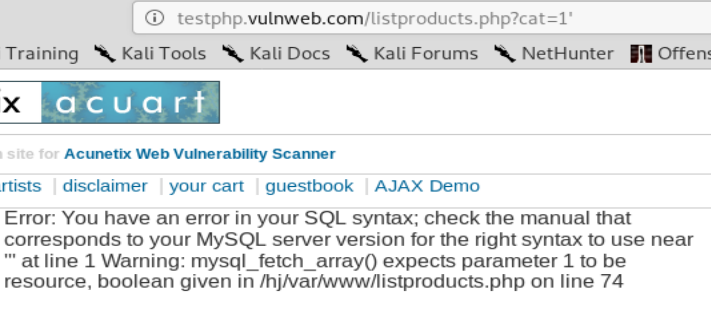
\includegraphics[width=0.7\textwidth]{oui/Ancien/imangeancien/Nikto/1.PNG}
  \caption{Scan simple}
  \label{fig:courbe-tikz}
\end{figure}

On peut remarquer grâce à cette capture wireshark que par défaut, Nikto scanne le port 80 :

\begin{figure}[htp!]
  \centering
  \setlength\figureheight{7cm}
  \setlength\figurewidth{9cm}
  
\includegraphics[width=0.7\textwidth]{oui/Ancien/imangeancien/Nikto/2.PNG}
  \caption{Scan d'un port}
  \label{fig:courbe-tikz}
\end{figure}

\begin{figure}[htp!]
  \centering
  \setlength\figureheight{7cm}
  \setlength\figurewidth{9cm}
  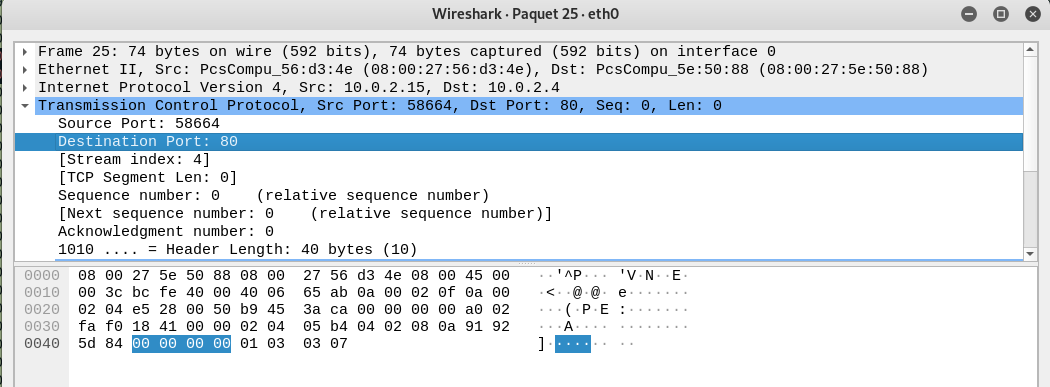
\includegraphics[width=0.7\textwidth]{oui/Ancien/imangeancien/Nikto/wireshark3.png}
  \caption{Mise en évidence du port scanné par défaut par la commande nikto}
  \label{fig:courbe-tikz}
\end{figure}

\newpage

Afin de scanner un port précis, il faut ajouter l'argument \textbf{-p}: 

\begin{figure}[htp!]
  \centering
  \setlength\figureheight{7cm}
  \setlength\figurewidth{9cm}
  
\includegraphics[width=0.8\textwidth]{oui/Ancien/imangeancien/Nikto/2.PNG}
  \caption{Scan d'un port}
  \label{fig:courbe-tikz}
\end{figure}

Dans cette capture, nous venons de scanner l'IP sur le port 80 (http). Il également possible de cibler plusieurs ports en même temps:


\begin{figure}[htp!]
  \centering
  \setlength\figureheight{7cm}
  \setlength\figurewidth{9cm}
  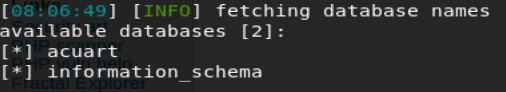
\includegraphics[width=0.8\textwidth]{oui/Ancien/imangeancien/Nikto/3.PNG}
  \caption{Scan de plusieurs ports}
  \label{fig:courbe-tikz}
\end{figure}

A partir de ces captures, on peut en déduire que Nikto est capable de nous fournir le logiciel qui permet de faire fonctionner le serveur web, sa version et également le système d'exploitation utilisé. En effet, toutes ces informations sont comprises dans l'entête des réponses HTTP du serveur. Nikto est également capable de vérifier les mauvaises configurations de services ou de programmes mal sécurisé. Cet outil propose également des plugins permettant la recherche d'autres vulnérabilités ou de fichier pouvant être intéressant dans un CTF tel que le fichier \textbf{robots.txt}. Ce fichier permet le référencement d'un site WEB par les robots de Google. Cependant, l'administrateur peut empêcher le scan de certains répertoires par les robots en précisant dans ce fichier quelques paramètres. Ainsi, grâce à cela, un attaquant peut utiliser ce fichier pour découvrir des répertoires que l'administrateur aurait voulu cacher.

\begin{figure}[htp!]
  \centering
  \setlength\figureheight{7cm}
  \setlength\figurewidth{9cm}
  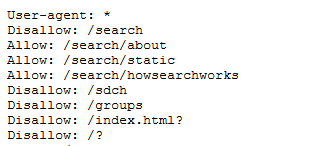
\includegraphics[width=0.5\textwidth]{oui/Ancien/imangeancien/Nikto/robots.PNG}
  \caption{Extrait fichier robots.txt}
  \label{fig:courbe-tikz}
\end{figure}

 On comprend à travers cette capture que le paramètre \textbf{Disallow} empêche le scan de ce répertoire.\\

\subsection{Gagner en discrétion pendant les scans}
Une méthode pour gagner en discrétion pendant l'attaque serait d'effectuer un scan par intervalle. En effet, si on effectue un scan toutes les 10 secondes, cela paraîtra moins suspect qu'un scan toutes les 1ms. Cela est possible en ajoutant l'option \textbf{-Pause 10} en argument :

\begin{figure}[htp!]
  \centering
  \setlength\figureheight{7cm}
  \setlength\figurewidth{9cm}
  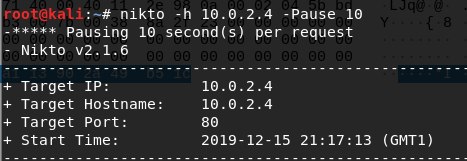
\includegraphics[width=0.8\textwidth]{oui/Ancien/imangeancien/Nikto/nikto9.png}
  \caption{Ajout de l'argument Pause}
  \label{fig:courbe-tikz}
\end{figure}

Voici une capture wireshark de ce scan avec l'ajout de l'argument :

\begin{figure}[htp!]
  \centering
  \setlength\figureheight{7cm}
  \setlength\figurewidth{9cm}
  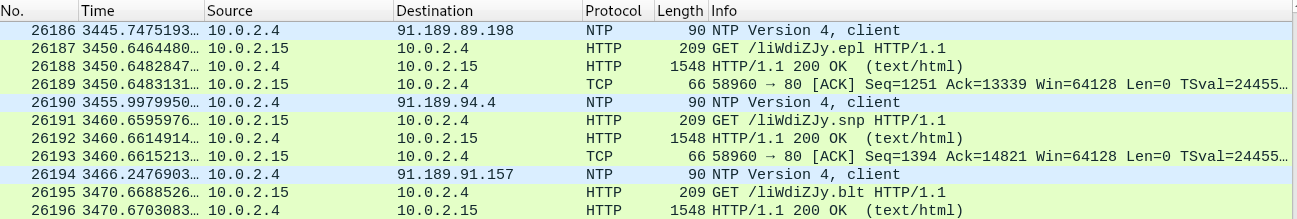
\includegraphics[width=1\textwidth]{oui/Ancien/imangeancien/Nikto/wireshark4.PNG}
  \caption{Capture wireshark du scan avec l'otpion de pause}
  \label{fig:courbe-tikz}
\end{figure}

 On remarque l'utilisation du protocole NTP (Network Time Protocol) qui permet ici de mettre en place le temps de pause.
\newpage

\section{Dirb/Dirbuster}

Après avoir réalisé un scan via Nmap et repéré qu'un serveur Web est activé, Dirb sera là pour vous guider à travers les pages car il est un scanneur de contenu Web. Son but est de trouver l’existence d’objets web, qu’ils soient cachés ou non.
Son fonctionnement réside en la lancée d’une attaque par dictionnaire contre un serveur web et d’en analyser la réponse. \\
Cependant, il existe une différence entre une attaque par dictionnaire et une attaque par bruteforce pure.\\
Une attaque par dictionnaire est une attaque que l’on utilise dans la cryptanalyse (technique de déduction d’un texte en clair par rapport à un texte chiffré sans la clé de chiffrement) pour justement trouver un mot de passe ou une clé de chiffrement. 
Son fonctionnement consiste à tester une liste donnée de mots de passe potentiels, un par un, en espérant que le mot de passe de chiffrement soit l’un deux. 
Cette technique ne marche donc pas systématiquement et il faut une énorme liste de mots de passe et du temps pour qu’elle soit efficace. L'intérêt d'installer des dictionnaires supplémentaires serait utile dans les cas de mots de passe très complexes.
C’est d’ailleurs à cause de ce genre d’attaque que l’on conseille de mettre des mots de passe compliqués, car ceux courants sont bien plus simples à trouver avec ce genre d’attaque. 

\subsection{Création de dictionnaires et utilisation de Dirb}

Comme nous l'avons plus haut, Dirb se base sur un dicitonnaire afin de réaliser son scan. Nous avons donc quatre possibilités :

\begin{itemize}
    \item \textbf{Créer un dictionnaire à partir d'une page Web}
    \item \textbf{Créer un dictionnaire sous forme de pattern}
    \item \textbf{Créer un dictionnaire aléatoire}
    \item \textbf{Utiliser un dictionnaire présent dans le répertoire de Dirb}\\
\end{itemize}

 \textbf{Créer un dictionnaire à partir d'une page Web}\\

Cette méthode est plus utilisée avec l'outil John que Dirb mais il est important de l'expliquer ici. En effet, utiliser des mots présents sur une page Web peut être intéressant dans le cas où nous avons un mot de passe hasher à découvrir. Il vous faudra donc télécharger la page Web en question via un wget et réaliser la commande suivante :

\begin{figure}[htp!]
  \centering
  \setlength\figureheight{7cm}
  \setlength\figurewidth{9cm}
  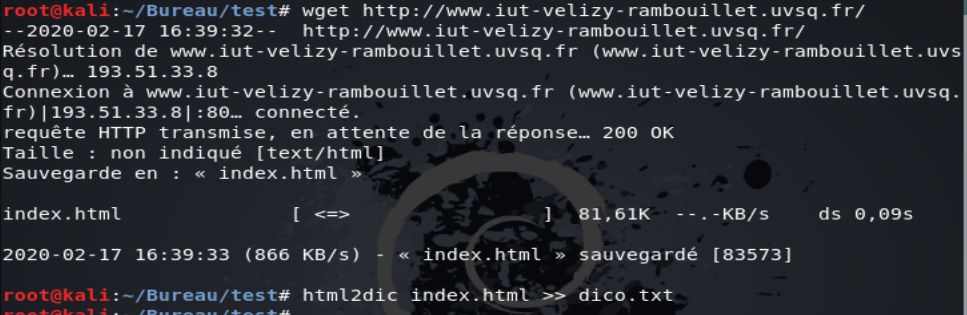
\includegraphics[width=1\textwidth]{oui/images/Dirb/html2dic.PNG}
  \caption{Html2dic}
  \label{fig:courbe-tikz}
\end{figure}

\newpage
C'est ainsi que nous pouvons créer un premier dictionnaire assez rapidement.\\

 \textbf{Créer un dictionnaire sous forme de pattern}\\

Lorsque que l'on connaît une partie du mot ou page que l'on recherche, utiliser un pattern peut être la solution. Un pattern est une forme commune qui va varier sur une partie pré-définie. Gendict est l'outil de création de dictionnaire avec pattern que nous allons utiliser ici. Il vous faudra cependant l'installer via le paquet "icu-devtools". Voici son utilisation :

\begin{figure}[htp!]
  \centering
  \setlength\figureheight{7cm}
  \setlength\figurewidth{9cm}
  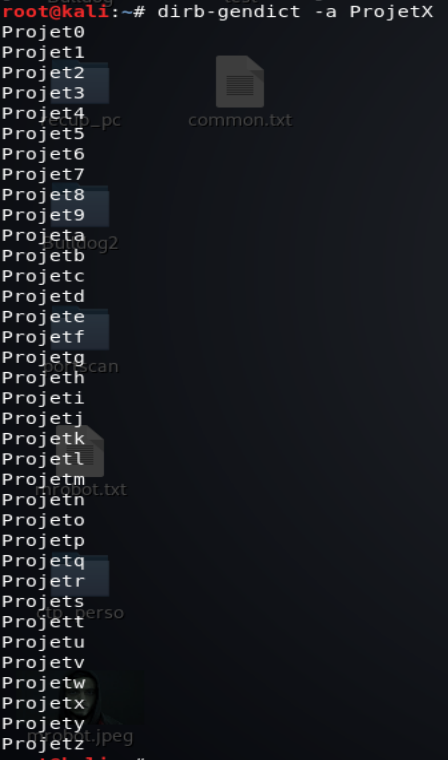
\includegraphics[width=0.34\textwidth]{oui/images/Dirb/gendict.PNG}
  \caption{Gendict -a}
  \label{fig:courbe-tikz}
\end{figure}

On comprend ici que le X sera la variable du pattern. Il est donc tout à fait possible de créer un dictionnaire sans pattern en mettant un nombre de X correspondant à la taille recherchée comme ceci :

\begin{figure}[htp!]
  \centering
  \setlength\figureheight{7cm}
  \setlength\figurewidth{9cm}
  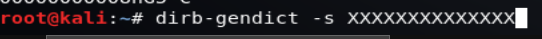
\includegraphics[width=0.9\textwidth]{oui/images/Dirb/dicoaleatoire.PNG}
  \caption{Gendict -s}
  \label{fig:courbe-tikz}
\end{figure}

L'option -s permet d'obtenir aussi les majuscules. Les deux principaux défauts de Gendict en tant que créateur de dictionnaires aléatoires sont les suivants :

\begin{itemize}
    \item \textbf{Le manque de caractères spéciaux}
    \item \textbf{La taille est fixe en fonction du nombre de X}
\end{itemize}

C'est pour cette raison qu'il existe un autre outil spécialisé dans la conception de dictionnaires aléatoires.\\

 \textbf{Créer un dictionnaire aléatoire}\\

L'outil que nous considérons comme le plus efficace en terme de création de dictionnaires aléatoires est l'outil Crunch. Ce dernier, en plus de réaliser du pattern, complète les défauts de Gendict. Nous allons vous présenter la manière pour réaliser le dictionnaire le plus complet possible de manière aléatoire. Tout d'abord, Crunch se base sur un dictionnaire se nommant "charset.lst". Vous y retrouverez les séries de caractères que vous pouvez choisir pour réaliser votre dictionnaire. Dans notre cas, nous avons choisis d'utiliser la série mixalpha-numeric-all-space et nous l'avons enregistré dans un fichier dico.txt comme ci-dessous :

\begin{figure}[htp!]
  \centering
  \setlength\figureheight{7cm}
  \setlength\figurewidth{9cm}
  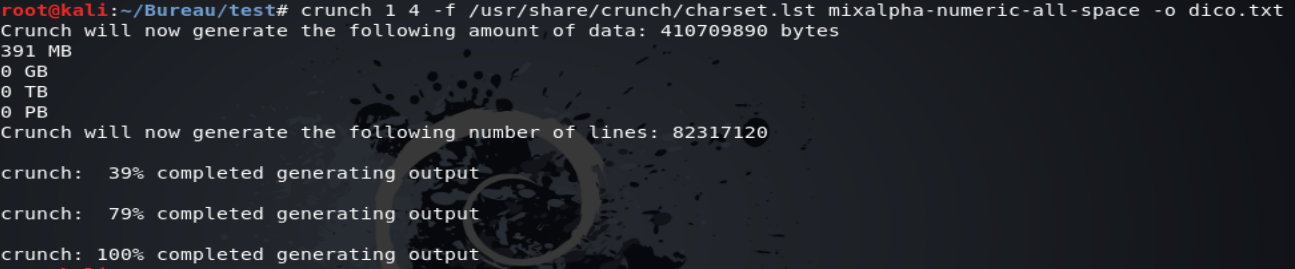
\includegraphics[width=1\textwidth]{oui/images/Dirb/crunch.PNG}
  \caption{Crunch}
  \label{fig:courbe-tikz}
\end{figure}

Comme vous pouvez le voir au début de la commande, nous avons spécifié que les mots devaient être générés entre 1 et 4 caractères et l'outil nous annonce que le dictionnaire fera 391 MB ! Pour information, les sites Web demandent en général un mot de passe avec au minimum 8 caractères. Je vous laisse donc lire la taille du dictionnaire si l'on souhaitait des mots de 1 à  8 caractères :

\begin{figure}[htp!]
  \centering
  \setlength\figureheight{7cm}
  \setlength\figurewidth{9cm}
  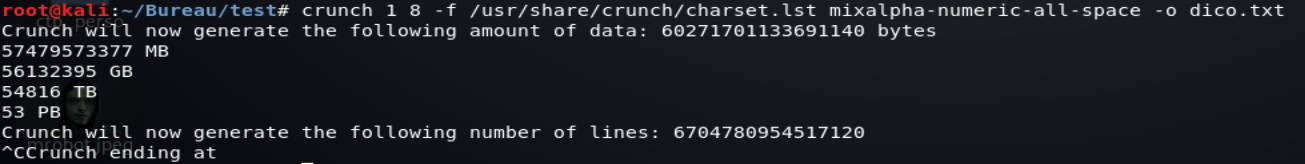
\includegraphics[width=1\textwidth]{oui/images/Dirb/crunch2.PNG}
  \caption{Crunch}
  \label{fig:courbe-tikz}
\end{figure}

Il est donc certain que cet outil vous permettra d'avoir un dictionnaire le plus complet au monde à la seule condition d'avoir une très grosse station de stockage... Heureusement que les concepteurs de Dirb ont pensé à ce détail et nous ont fourni des dictionnaires par défaut.\\

 \textbf{Utiliser un dictionnaire présent dans le répertoire de Dirb}\\

Comme nous l'avons vu précedemment, créer un dictionnaire peut vite devenir fastidieux. C'est pour cette raison que nous allons nous baser sur les dictionnaires présents dans le répertoire de Dirb. Il en existe plusieurs mais ici, nous allons utiliser le dictionnaire common.txt :

\begin{figure}[htp!]
  \centering
  \setlength\figureheight{7cm}
  \setlength\figurewidth{9cm}
  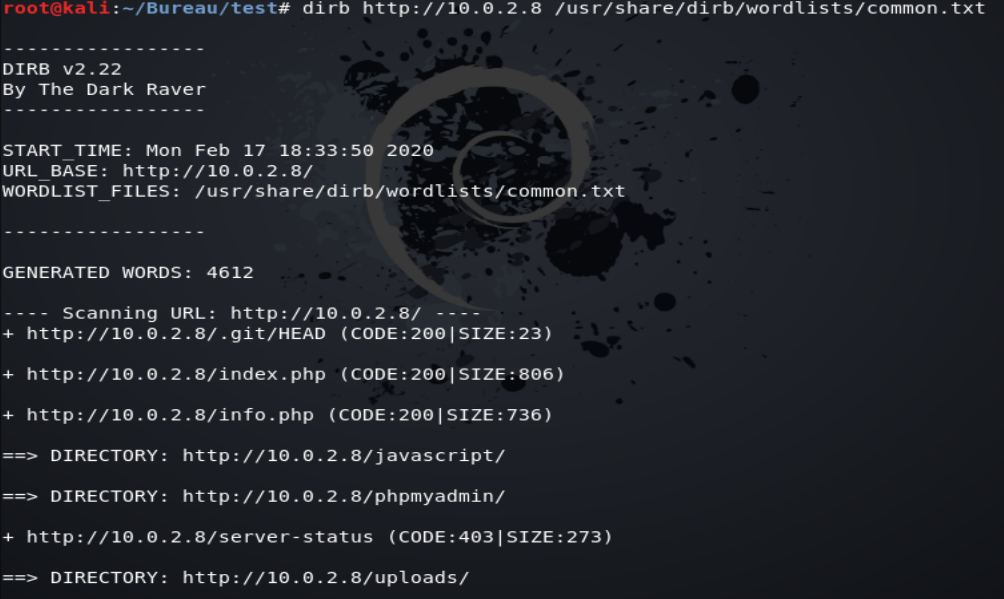
\includegraphics[width=1\textwidth]{oui/images/Dirb/dirb.PNG}
  \caption{Utilisation de Dirb}
  \label{fig:courbe-tikz}
\end{figure}

Encore une fois, l'utilisation d'un dictionnaire est très personnel. Il vous suffira donc de changer le dictionnaire et de lancer la commande afin d'obtenir un résultat. Comme vos pouvez le voir sur la capture d'écran ci-dessus, Dirb nous donne des pages cachées que nous n'aurions pas forcément trouvé tout seul. Cet outil est donc essentiel lors d'un pentest Web.

\subsection{Comparaison entre Dirb et Dirbuster}

Pour ceux qui préfèrent les interfaces graphiques aux lignes de commandes, il existe l'équivalent de Dirb en GUI (Graphical User Interface) qui se nomme Dirbuster.

Ce dernier permet, lui aussi, d’attaquer un site par dictionnaire. Il suffit de rentrer l'adresse IP du site ainsi que le répertoire où est stocké la liste de mots visible en \textbf{figure \ref{fig:dirbuster}}. 

\begin{figure}[htp!]
  \centering
  \setlength\figureheight{7cm}
  \setlength\figurewidth{9cm}
  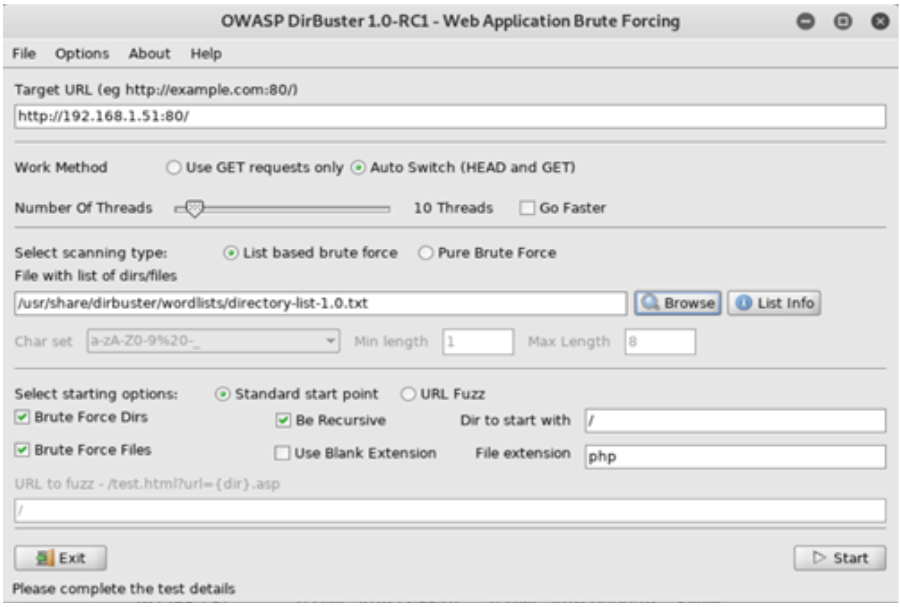
\includegraphics[width=0.8\textwidth]{oui/Ancien/imangeancien/dirb1.PNG}
  \caption{Dirbuster}
  \label{fig:dirbuster}
\end{figure}

L’utilisation de Dirb et Dirbuster est fondamentalement la même, mais ils ont chacun leurs avantages. 

Tout d’abord pour la question de rapidité, Dirb est en single-threading alors que Dirbuster est en multi-threading. \\
La différence entre single et multi est qu’en single, on ne peut exécuter les tâches qu’une par une de la manière suivante : 
\begin{center}
   \begin{figure}[htp!]
  \centering
  \setlength\figureheight{7cm}
  \setlength\figurewidth{9cm}
  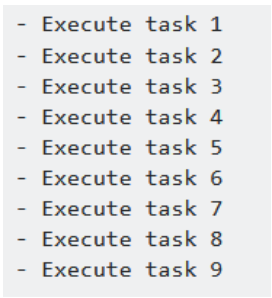
\includegraphics[width=0.25\textwidth]{oui/Ancien/imangeancien/dirb3.PNG}
  \caption{Single-threading}
  \label{fig:courbe-tikz}
\end{figure} 
\end{center}

 Alors que le multi-threading, lui, permet de faire plusieurs tâches en même temps en ordonnant les tâches en plusieurs threads, de la manière suivante : 
\begin{center}
    \textbf{Thread1}:\\
       \begin{figure}[htp!]
  \centering
  \setlength\figureheight{7cm}
  \setlength\figurewidth{9cm}
  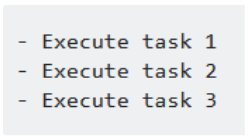
\includegraphics[width=0.25\textwidth]{oui/Ancien/imangeancien/dirb4.PNG}
  \label{fig:courbe-tikz}
\end{figure}
\textbf{Thread2}:\\
       \begin{figure}[htp!]
  \centering
  \setlength\figureheight{7cm}
  \setlength\figurewidth{9cm}
  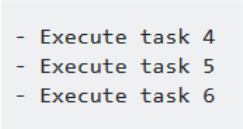
\includegraphics[width=0.25\textwidth]{oui/Ancien/imangeancien/dirb5.PNG}
  \label{fig:courbe-tikz}
\end{figure}

\textbf{Thread3}:\\
       \begin{figure}[htp!]
  \centering
  \setlength\figureheight{7cm}
  \setlength\figurewidth{9cm}
  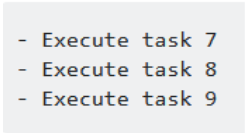
\includegraphics[width=0.25\textwidth]{oui/Ancien/imangeancien/dirb6.PNG}
  \caption{Multi-threading}
  \label{fig:courbe-tikz}
\end{figure}
\end{center}
Il faut noter que la différence ne se voit qu’avec des processeurs multi-coeurs, qui peuvent faire plusieurs tâches à la fois. \\
Donc pour la rapidité d’exécution, si nous avons un bon processeur, Dirbuster surpasse largement Dirb.
Seulement, Dirbuster demande toujours une interaction graphique, alors que Dirb, étant une CLI (Command Line Interface), permet l’automatisation, donc on perd certes du temps sur l’exécution des tâches mais on gagne du temps sur le reste.\\
Certes, Dirb vous fournira les fichiers tel que robots.txt mais ne fournira pas le code source des pages. N'hésitez pas à les observer car elles contiennent beaucoup d'informations. 
%\chapter{Premier pas dans un CTF}
\label{chap:BDD}

    Nous voici donc partis pour notre premier CTF. En général, l’adresse IP de la machine cible sera fournie mais au cas où ça ne serait pas le cas, nous vous conseillons d’utiliser un ‘arp-scan --localnet’ comme ceci :

%Image arp-scan
\begin{figure}[htp!]
  \centering
  \setlength\figureheight{7cm}
  \setlength\figurewidth{9cm}
  \includegraphics[width=1\textwidth]{oui/Screens/unknown.png}
  \caption{ARP-SCAN}
  \label{fig:courbe-tikz}
\end{figure}

Si la machine cible est connue sous un nom DNS, il est possible, soit de ping ce nom ou bien de réaliser un nslookup que nous allons privilégier. Comme on peut le voir ci-dessous, nous pouvons retrouver l'addresse IPV4 et IPV6 d'une machine connue sous son nom :

\begin{figure}[htp!]
  \centering
  \setlength\figureheight{7cm}
  \setlength\figurewidth{9cm}
  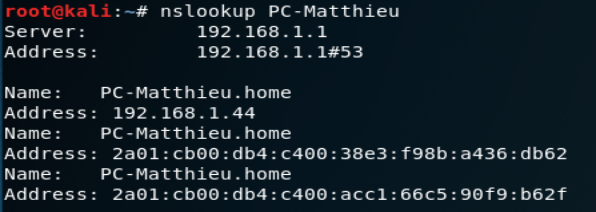
\includegraphics[width=0.6\textwidth]{oui/Screens/nslookup.PNG}
  \caption{Nslookup}
  \label{fig:courbe-tikz}
\end{figure}

\newpage
\section{ARP-Scan}
Arp-scan est un utilitaire qui permet  d’obtenir les adresses IP d’un réseau via la couche 2 du modèle OSI . Le modèle OSI est une norme d’exemple pour tous les types de transmissions réseaux. Ce modèle peut être vu de cette manière :
%Image modèle OSI
\begin{figure}[htp!]
  \centering
  \setlength\figureheight{7cm}
  \setlength\figurewidth{9cm}
  \includegraphics[width=0.3\textwidth]{oui/Screens/modeleOSI.PNG}
  \caption{Schéma du modèle OSI}
  \label{fig:courbe-tikz}
\end{figure}

La couche 2 est la couche de liaison de données. Cette dernière correspond à l’adressage physique des machines, soit l’adresse MAC. L’adresse MAC est l’adresse unique d’une interface réseau d’un équipement. Cette adresse est codée en hexadécimal en 6 octets.

\subsection{Fonctionnement d'ARP-Scan}

Ce dernier va envoyer une requête ARP en broadcast sur le réseau et afficher l’IP, l'adresse MAC ainsi que, si possible, l'origine de chaque hôte. Si un hôte ne répond pas, le paquet ARP sera envoyé à nouveau. Le nombre maximum de tentatives peut être modifié avec l'option --retry. Cependant, si l'on réduit le nombre de tentatives, alors cela réduira le temps du scan mais engendrera le risque de perdre certains résultats en raison de la perte de paquets.
Comme vous pouvez le voir ci-dessous, la capture Wireshark faite à la suite d’un ‘arp-scan’ se présente de la même manière qu’une requête ARP : 

%Image Wireshark arp broadcast
\begin{figure}[htp!]
  \centering
  \setlength\figureheight{7cm}
  \setlength\figurewidth{9cm}
  
\includegraphics[width=1\textwidth]{oui/Screens/wireshark.PNG}
  \caption{Capture Wireshark}
  \label{fig:courbe-tikz}
\end{figure}

\newpage
Le protocole ARP est un protocole de niveau 2 (couche de liaison de données) qui est utilisé pour déterminer l'adresse MAC (couche 2) d'un hôte distant à partir de son adresse IP (couche 3). L'ARP a été conçu pour fonctionner avec n'importe quel format d'adresse de couche 2 et de couche 3, mais l'utilisation la plus courante est de cartographier un réseau.
Cependant, cet outil ne peut être utilisé que sur des réseaux LAN car les requêtes ARP ne peuvent pas être routées dans le cas d’un scan de réseau Local.
Ce protocole utilise des adresses IP, mais il n'est pas basé sur IP. Ainsi, arp-scan peut être utilisé sur une interface qui n'est pas configurée pour IP.
Nous voici avec les adresses IP et MAC de la cible.
Le seul et unique moyen de s’infiltrer dans une machine est de s’introduire via les ports ouverts de cette dernière. Il nous faudra donc faire une analyse de ports en fonction de l’IP avec l’utilitaire Nmap comme ceci :

%Image nmap
\begin{figure}[htp!]
  \centering
  \setlength\figureheight{7cm}
  \setlength\figurewidth{9cm}
  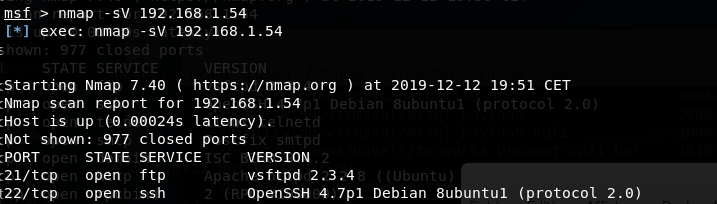
\includegraphics[width=0.75\textwidth]{oui/Screens/nmap.PNG}
  \caption{Utilisation de Nmap}
  \label{fig:courbe-tikz}
\end{figure}
À partir de nmap, on obtient tous les ports ouverts sur la machine distante ainsi que les services qui sont actifs sur cette dernière. Par exemple, dans cette capture le port 22 qui correspond à SSH est ouvert ainsi que le port 80 qui correspond à un serveur HTTP (Apache). Cela veut dire que nous pouvons accéder à un serveur web depuis le navigateur en tapant dans l’URL “http://192.168.1.27”. De plus, nous pouvons nous connecter au serveur SSH sous réserve d’avoir des identifiants et un mot de passe. Mais à l’heure actuelle, nous n’avons rien de cela. Tout le but du CTF sera de récupérer ces informations ou de passer par des méthodes tierces dans le but de nous infiltrer dans la machine pour récupérer un ou des flags. Nous allons maintenant introduire les différents outils de scans de vulnérabilités. On appelle cela une récolte d’informations active car nous allons entrer directement en relation avec la cible afin d’obtenir des informations utilisables. Tandis qu’une récolte d’informations passive consiste à chercher des informations sur la cible directement sur le web avec des outils comme “whois” pour récupérer des adresses IP ou des DNS ou avec “NSLookup” pour interroger un serveur DNS et obtenir des enregistrements sur les différents hôtes qu’il connaît.
%\chapter{Les outils de Scans}
\label{chap:BDD}

Lors d'une attaque, le scan est une obligation pour savoir où attaquer la cible. En effet, que ce soit pour découvrir les ports ouverts ou pour savoir quelles vulnérabilités sont présentes, nous aurons besoin d'un scanneur. Nous vous présenterons dans un premier temps un scanneur de port qui sera Nmap. Puis nous allons vous présenter l'outil Nikto pour ce qui est du scan de vulnérabilités d'un site Web.

\section{Nmap}
\subsection{Présentation de Nmap}
Nmap est un utilitaire permettant de scanner les ports ouverts d’une machine ou d’un ensemble de machines présentes dans un même réseau. Chaque programme voulant émettre sur le réseau va devoir sortir de son hôte. Chacun d’eux va se voir alors attribuer une porte pour sortir et qui devra rester ouverte tant qu’ils voudront émettre. Ces portes sont les ports ouverts d’une machine. En trouvant ces ports, Nmap se rend comme l’élément essentiel d’une attaque réseau. En effet, sans cette analyse, nous serions incapable de trouver un chemin d’attaque à moins d’avoir une chance inouïe. C’est pourquoi nous allons utiliser cet utilitaire pour résoudre nos CTFs.



\subsection{Fonctionnement de Nmap}
Tout d’abord, Nmap peut être utilisée en lui renseignant qu’une adresse IP sans option comme ceci :
\begin{figure}[htp!]
  \centering
  \setlength\figureheight{7cm}
  \setlength\figurewidth{9cm}
  \includegraphics[width=0.7\textwidth]{oui/Screens/nmap/justeip.PNG}
  \caption{Utilisation de nmap sans options}
  \label{fig:courbe-tikz}
\end{figure}

\newpage
Cette commande intuitive et rapide nous permet d’obtenir le port ouvert ainsi que le protocole qui lui est associé. Cependant, il serait intéressant pour une futur exploitation de faille, d’obtenir le nom du \textbf{S}erveur web ainsi que sa \textbf{V}ersion. C’est pourquoi nous allons appliquer l’argument ‘ -sV ‘ :
\begin{figure}[htp!]
  \centering
  \setlength\figureheight{7cm}
  \setlength\figurewidth{9cm}
  \includegraphics[width=1\textwidth]{oui/Screens/nmap/-sV.PNG}
  \caption{Ajout de l'opton -sV}
  \label{fig:courbe-tikz}
\end{figure}

Le CTF analysé ici utilise un serveur web nginx de version $1.14.0$. Nous ne pouvons que vous conseiller de garder ce type d’informations dans un bloc-note tout au long d’une attaque.\\
Nous pouvons à partir de ce résultat se demander comment Nmap récupère les informations concernant la version des serveurs. Tout d'abord, Il faut savoir que cet outil travaille sur deux base données : une pour les ports et une autre pour les versions des logiciels et serveurs. Pour ce qui est des ports, la base de données se nomme 'nmap-service' et est visualisable via ce lien :\\
https://svn.nmap.org/nmap/nmap-services\\
La base de données pour les versions est 'nmap-service-probes' :\\
https://svn.nmap.org/nmap/nmap-service-probes\\
Afin de comprendre comment Nmap exploite ces dictionnaires, nous avons réécrit en Python un programme scannant les ports d'un serveur Samba et affichant la version du protocole utilisé. Il faut savoir avant d'observer le programme que Nmap utilise des regex afin de comparer la réponse envoyée par le serveur et ainsi obtenir la version. Voici notre programme :

\begin{figure}[htp!]
  \centering
  \setlength\figureheight{7cm}
  \setlength\figurewidth{9cm}
  \includegraphics[width=0.9\textwidth]{oui/Screens/nmap/Part1.PNG}
  \caption{Scanneur Samba partie 1}
  \label{fig:courbe-tikz}
\end{figure}

\begin{figure}[htp!]
  \centering
  \setlength\figureheight{7cm}
  \setlength\figurewidth{9cm}
  \includegraphics[width=0.9\textwidth]{oui/Screens/nmap/Part2.PNG}
  \caption{Scanneur Samba partie 2}
  \label{fig:courbe-tikz}
\end{figure}

\newpage
Lors de son exécution, on voit apparaître le nom du service, son port ainsi que sa version. On peut comparer son exécution avec Nmap :

\begin{figure}[htp!]
  \centering
  \setlength\figureheight{7cm}
  \setlength\figurewidth{9cm}
  \includegraphics[width=0.9\textwidth]{oui/Screens/nmap/Result.PNG}
  \caption{Scanneur Samba}
  \label{fig:courbe-tikz}
\end{figure}

\newpages
On remarque que notre programme affiche les résultats en 0.34 secondes contre en 11.89 secondes avec Nmap. On suppose que Nmap réalise d'autres calculs en arrière plan pour obtenir une vérification de la version. Voici une différence entre notre programme et Nmap au niveau de Wireshark :

\begin{figure}[htp!]
  \centering
  \setlength\figureheight{7cm}
  \setlength\figurewidth{9cm}
  \includegraphics[width=0.9\textwidth]{oui/Screens/nmap/wireshark_prog.PNG}
  \caption{Gauche : Python et Droite : Nmap}
  \label{fig:courbe-tikz}
\end{figure}

En effet, Nmap réalise un RST après avoir testé l'ouverture du port pour réinitialiser la connexion du socket. C'est alors après qu'il lance une séquence d'initialisation TCP (SYN, SYN ACK, ACK) afin d'envoyer sa requête au serveur via le protocole SMB. Ce dernier lui renvoie une valeur incompréhensible par l'homme qu'il faut décoder pour le matcher avec la base de données de Nmap. C'est ainsi que Nmap opère pour récupérer la version du protocole utilisée.


\newpage
Maintenant que nous avons vu comment utiliser basiquement Nmap, nous pouvons nous demander comment fonctionne cet utilitaire. En effet, il est obligé de faire des requêtes sur tous les ports en utilisant le protocole ICMP, IP, TCP et UDP. Cet utilitaire utilise donc les couches 3 et 4 du modèle OSI.\\
Cependant, en émettant toutes ses requêtes, Nmap laisse des traces :
\begin{figure}[htp!]
  \centering
  \setlength\figureheight{7cm}
  \setlength\figurewidth{9cm}
  \includegraphics[width=0.85\textwidth]{oui/Screens/nmap/Wiresharkhypervisible.PNG}
  \caption{Scan avec wireshak}
  \label{fig:courbe-tikz}
\end{figure}

Nous allons donc voir comment éviter de nous faire "trop" repérer sur le réseau.\\
Dans un premier temps, nous pouvons fragmenter nos paquets avec l’option ‘ -f ‘ :
\begin{figure}[htp!]
  \centering
  \setlength\figureheight{7cm}
  \setlength\figurewidth{9cm}
  \includegraphics[width=1\textwidth]{oui/Screens/nmap/-f.PNG}
  \caption{Ajout de l'option -f}
  \label{fig:courbe-tikz}
\end{figure}

Cette option va fragmenter nos paquets pour les éparpiller sur le réseau et ainsi ne pas indiquer tout de suite que nous scannons le port 80 comme avant :
\begin{figure}[htp!]
  \centering
  \setlength\figureheight{7cm}
  \setlength\figurewidth{9cm}
  \includegraphics[width=0.75\textwidth]{oui/Screens/nmap/Wireshark-f-Copie.PNG}
  \caption{Scan avec wireshak en ajoutant l'option -f}
  \label{fig:courbe-tikz}
\end{figure}

\newpage
La capture Wireshark ci-dessus nous montre qu’en fragmentant nos paquets, nous utilisons le protocole IP et TCP. De plus, cette fragmentation permet de noyer le scan de ports ( les [SYN] ) et d’outrepasser un firewall. En effet, de vieux firewalls peuvent avoir des failles comme celles de la fragmentation. Ces derniers étaient incapables de s’en occuper donc les laissaient passer. Cependant, les programmeurs ont résolus le problème donc cette faille n’est plus exploitable sur les nouveaux firewalls. C'est pour cette raison que nous n'allons pas détailler cette méthode fragmentation.\\
Comme nous l'avons vu, Nmap se fait passer un client lambda via ses requêtes. Cependant, il envoie par défaut un nombre de requêtes par seconde qui n'est pas réalisable par un humain. Cette vitesse d'envoi par défaut est le T3 qui scanne un port toutes les 16 ms ce qui provoque une alarme chez les firewalls. Voici un tableau qui répertorie la vitesse de scan pour un port :

\begin{figure}[htp!]
  \centering
  \setlength\figureheight{7cm}
  \setlength\figurewidth{9cm}
  \includegraphics[width=1\textwidth]{oui/Screens/nmap/tableau.PNG}
  \caption{Tableau vitesse de scan}
  \label{fig:courbe-tikz}
\end{figure}

Les valeurs de ce tableau peuvent varier en fonction du processeur, de la quantité de RAM et du débit sur le réseau. On peut remarquer le T0 et le T1 peuvent se faire passer pour un humain et seront donc utilisés pour être indétectables par les firewalls. Cependant, ce scan, même en T1, risque de prendre énormément de temps. Si on pose le calcul théorique, notre scan en T1, le plus rapide des indétectables, prendrai 50 heures pour scanner les mille premiers ports.
 

\newpage
Nous commençons à avoir une belle couverture de nos traces sur le réseau. Mais nous allons essayer de faire mieux en usurpant une adresse MAC du réseau pour passer pour un autre :

\begin{figure}[htp!]
  \centering
  \setlength\figureheight{7cm}
  \setlength\figurewidth{9cm}
  \includegraphics[width=1\textwidth]{oui/Screens/nmap/spoof-mac.PNG}
  \caption{Usurpation d'adresse MAC}
  \label{fig:courbe-tikz}
\end{figure}

L’option ‘ --spoof-mac ‘ nous permet de remplacer notre adresse MAC par celle renseignée en argument de l’option. Voici comment réagit Wireshark face à ce changement :

\begin{figure}[htp!]
  \centering
  \setlength\figureheight{7cm}
  \setlength\figurewidth{9cm}
  \includegraphics[width=1\textwidth]{oui/Screens/nmap/Wiresharkspoofmac.PNG}
  \caption{Wireshark usurpation MAC}
  \label{fig:courbe-tikz}
\end{figure}

Allons encore plus loin en usurpant l’IP d’une autre machine :

\begin{figure}[htp!]
  \centering
  \setlength\figureheight{7cm}
  \setlength\figurewidth{9cm}
  \includegraphics[width=1\textwidth]{oui/Screens/nmap/spoofipetmac.PNG}
  \caption{Usurpation MAC et IP}
  \label{fig:courbe-tikz}
\end{figure}

De cette manière, nous avons pu faire simuler un Nmap à partir du Raspberry présent sur le réseau. L’option ‘ -S ‘ permet d’associer une IP source au paquet. Cette option doit être accompagnée d'un ‘ -g ‘ pour lui indiquer le port de sorti ainsi que de l’option ‘ -e ‘ pour informer notre interface réseau. Nmap nous recommande d’utiliser l’option ‘ -Pn ‘ pour considérer que tous les hôtes sont en ligne.
Nous obtenons un Wireshark vide entre notre machine et la cible.
Si nous observons une capture de trafic entre le Raspberry et la cible :

\begin{figure}[htp!]
  \centering
  \setlength\figureheight{7cm}
  \setlength\figurewidth{9cm}
  \includegraphics[width=1\textwidth]{oui/Screens/nmap/Wiresharkusurpe.PNG}
  \caption{Wireshark usurpation MAC et IP}
  \label{fig:courbe-tikz}
\end{figure}

\noindent Nos paquets fragmentés sont bien envoyés entre les deux et nous recevons la réponse de notre scan sans être impliqué dans la ‘discussion’.
Notre scan est alors une réussite.\\
Mais comment avons nous pu récupérer ces informations sans être présent dans les discutions ? Comme nous l'avons vu plus haut, l'option '-e ' a pour but d'informer Nmap de faire sortir et entrer les informations via un port que l'on ouvre sur notre machine. Via ce procédé, notre interface va envoyer et recevoir les paquets échangés entre la machine cible et celle usurpée.  Ainsi, nous nous plaçons tel un proxy et nous récupérons en ‘man-in-the-middle’ les informations sans être vu. Il y a plusieurs types d’attaques ‘man-in-the-middle’. Ici, nous utilisons le type d’attaque ‘ARP spoofing’ en usurpant les adresses d’une machine dans le même réseau que la machine cible et en forçant les communications à transiter par notre machine virtuelle en se faisant passer pour un relais.

\subsection{Réaction d'un firewall Stormshield face à Nmap}

Au cours de cette présentation de Nmap, nous n'avions aucune sécurité présente entre la l'attaquant et la cible. Nous allons donc réaliser une attaque d'un réseau à l'autre avec pour routeur un firewall Stormshield. Un firewall est un équipement physique ou non, qui permet de sécuriser les entrées et les sorties d'un réseau. Nous allons ici utiliser un firewall Stormshield SN210W qui est un équipement physique. Voici la topologie utilisée lors de ces essais :

\begin{figure}[htp!]
  \centering
  \setlength\figureheight{7cm}
  \setlength\figurewidth{9cm}
  \includegraphics[width=1\textwidth]{oui/Screens/nmap/FirewallDiagram.png}
  \caption{Topologie}
  \label{fig:courbe-tikz}
\end{figure}

\newpage
Nous avons utilisé la configuration d'usine du firewall afin d'avoir un point de vue objectif face à Nmap. Au cours de ces essais, nous allons utiliser une attaque témoin qui sera l'attaque sans option de Nmap. Nous pouvons alors regarder les logs du firewall à la suite de cette attaque :

\begin{figure}[htp!]
  \centering
  \setlength\figureheight{7cm}
  \setlength\figurewidth{9cm}
  \includegraphics[width=0.9\textwidth]{oui/Screens/nmap/stormshield/alarme_nmap_base.PNG}
  \caption{Log Stormshield face à un Nmap sans option}
  \label{fig:courbe-tikz}
\end{figure}

\newpage
Le firewall détecte très facilement la présence de Nmap et bloque les requêtes ICMP faites par l'attaquant. Cependant, nous pouvons observer une faille au niveau des requêtes SYN car le firewall les laisse passer. Pour confirmer cette théorie, nous avons fais une requête de versions qui s'est aboutie en 152,93 secondes. Nous ne pouvons pas afficher les alarmes tellement les firewall en a déclaré. Cependant, encore une fois, Nmap était détecté et les SYN sont passés. Nous allons donc forcer Nmap à effectuer un scan en utilisant que des SYN avec la comande '-sS' :

\begin{figure}[htp!]
  \centering
  \setlength\figureheight{7cm}
  \setlength\figurewidth{9cm}
  \includegraphics[width=0.9\textwidth]{oui/Screens/nmap/stormshield/Alarme-sS.PNG}
  \caption{Log Stormshield face à un Nmap -sS}
  \label{fig:courbe-tikz}
\end{figure}

Ce scan s'est terminé en 14,43 secondes ce qui est en moyenne plus long qu'un scan sans option. Cependant, le résultat est concluant car le firewall ne détecte plus la présence de Nmap. Nous allons procéder de la même manière afin de récupérer les versions :

\begin{figure}[htp!]
  \centering
  \setlength\figureheight{7cm}
  \setlength\figurewidth{9cm}
  \includegraphics[width=0.9\textwidth]{oui/Screens/nmap/stormshield/result-sS-sV.PNG}
  \caption{Log Stormshield face à un Nmap -sS -sV}
  \label{fig:courbe-tikz}
\end{figure}

\newpage
Le scan s'est terminé en 63,72 secondes soit un gain de 58,33\% de temps comparé au scan de version standard. De plus, le nombre à diminué de plus de moitié, ce qui permet de les afficher ci-dessus. On peut remarquer que le plus gros nombre d'alarme se déclenche sur des requêtes DCERPC invalides. Le protocole DCE/RPC (Distributed Computing Environment /Remote Procedure Calls) permet des envois à distance comme pourrait faire un serveur Samba. Microsoft utilise énormément ce protocole pour mettre en place ses services. Or dans notre cas, la cible possède plusieurs services utilisant MS-RPC comme le montre le résultat du scan -sS -sV :

\begin{figure}[htp!]
  \centering
  \setlength\figureheight{7cm}
  \setlength\figurewidth{9cm}
  \includegraphics[width=0.9\textwidth]{oui/Screens/nmap/stormshield/commande-sS-sV.PNG}
  \caption{Nmap -sS -sV}
  \label{fig:courbe-tikz}
\end{figure}

Ceci nous montre que un ou plusieurs protocoles utilisés par Windows ne sont pas autorisés par le firewall. Certes, notre scan Nmap crée des alertes sur le firewall mais ces alertes seront presque invisibles après la configuration du Stromshield au sein d'une grande entreprise. En effet, soit l'administrateur réseau devra désactiver sur chaque ordinateur les services MS-RPC ou les autoriser sur le firewall afin de ne pas avoir d'alarmes intempestives. Etant donné le nombre de messages passant le firewall, nos messages pourront se mêler aux ceux des employés sans être vus.\\
Nous auront malheureusement du mal avec Nmap à camoufler notre IP. En effet, après avoir rajouter une machine en 192.168.1.11, nous avons réalisé un spoof IP et MAC pour attaquer notre cible. Cependant, notre firewall doit réaliser des requêtes sur le réseau bloquant ce système comme on peut le voir ci-dessous :

\begin{figure}[htp!]
  \centering
  \setlength\figureheight{7cm}
  \setlength\figurewidth{9cm}
  \includegraphics[width=0.9\textwidth]{oui/Screens/nmap/stormshield/screen_spoofmac.PNG}
  \caption{Spoof non fonctionnel}
  \label{fig:courbe-tikz}
\end{figure}

\newpage
Le Stromshield a écrit ceci dans sa CLI. On y comprend que le firewall fait des requêtes ARP afin de vérifier l'identité du client et annule notre spoof MAC.

\textbf{Conclusion}:\\
Nmap est un outil de scan de ports très puissant. Ce dernier a la capacité de nous faire disparaître des échanges réseaux tout en capturant les informations sur les ports de la cible.

\section{Nikto}

Lorsque les hackeurs ont pour objectif d’attaquer une cible, ils ont recours à un outil tel que Nikto afin de scanner les vulnérabilités et de passer le moins de temps possible à attaquer la cible à proprement parlé. Nikto est donc un outil permettant aux hackeurs de gagner du temps.
Nikto est un scanner de vulnérabilités web écrit en Perl et sous licence GPL. Il va permettre de tester la sécurité de la configuration d'un serveur web (les options HTTP, les index, les potentielles failles XSS, injections SQL etc…).\\
Avant de montrer ce que peut réaliser Nikto, nous pouvons dans un premier temps revoir comment fonctionne une requête Web. Parmis les ports réservés, les serveurs Web ont pour port 80 pour l'HTTP ou 443 pour l'HTTPS. Pour comprendre le fonctionnement, nous allons analyser un échange entre un client et un serveur :

\begin{figure}[htp!]
  \centering
  \setlength\figureheight{7cm}
  \setlength\figurewidth{9cm}
  \includegraphics[width=0.7\textwidth]{oui/Screens/Nikto/wEBDiagram.png}
  \caption{Échange entre un navigateur et un serveur Web}
  \label{fig:courbe-tikz}
\end{figure}

\newpage
Comme vous pouvez le voir, le schéma ci-dessus ainsi que la capture wireshark ci-dessous montrent l'échange minimal entre un navigateur et un serveur Web afin d'obtenir une page HTML via HTTP.Une page Web n'est pas une vidéo que l'on regarde en streaming ou un appel vidéo qui utilise le protocole de transport UDP pour transmettre les paquets. En effet, lorsque nous chargeons une page Web, nous la voulons complète et sans erreurs. C'est pourquoi le protocole TCP existe. Sur notre diagramme d'échange, nous pouvons observer que le protocole TCP est présent lors des trois premiers échanges (SYN, SYN ACK, ACK). Ces échanges TCP se nomment 3-Way-Handshake, qui peut se traduire par : "les trois échanges pour se mettre d'accord sur la connexion". Il faut comprendre que après chaque échange, le protocole TCP prévoit un ACK (acquittement) pour annoncer que le paquets a été reçu sans erreurs. Maintenant que nous avons compris TCP, nous pouvons passer à la couche applicative de cet échange : le HTTP. Les envois HTTP sont directement émis par le navigateur et par le serveur Web. Ici, c'est notre navigateur qui fait une requête GET au serveur pour obtenir l'ensemble de la page Web voulue. Il existe plusieurs types de requêtes Web (GET, POST, HEAD, ...) mais seul le GET va nous intéresser car il est le plus utilisé. 

\begin{figure}[htp!]
  \centering
  \setlength\figureheight{7cm}
  \setlength\figurewidth{9cm}
  \includegraphics[width=0.7\textwidth]{oui/Screens/Nikto/wireshark1.png}
  \caption{Capture Wireshark d'un scan nikto}
  \label{fig:courbe-tikz}
\end{figure}

\newpage
Lors du scan, Nikto est capable de :\\
\textbf{- Vérifier}     si la version du serveur est obsolète ainsi que les logiciels et     modules qui sont utilisés par ce dernier. \\   
\textbf{- Scanner}     les répertoires, qui peuvent contenir des informations sensibles.\\
\textbf{- Tester}     près de 6000 fichiers potentiellement vulnérables.\\
De plus, Nikto supporte les connections SSL.

\subsection{Utilisation de Nikto}
Pour lancer un simple scan, il suffit de réaliser la commande :

\begin{figure}[htp!]
  \centering
  \setlength\figureheight{7cm}
  \setlength\figurewidth{9cm}
  \includegraphics[width=0.8\textwidth]{oui/Screens/Nikto/1.PNG}
  \caption{Scan simple}
  \label{fig:courbe-tikz}
\end{figure}

\begin{figure}[htp!]
  \centering
  \setlength\figureheight{7cm}
  \setlength\figurewidth{9cm}
  \includegraphics[width=0.8\textwidth]{oui/Screens/Nikto/wireshark3.png}
  \caption{Mise en évidence du port scanné par défaut par la commande nikto}
  \label{fig:courbe-tikz}
\end{figure}

On peut remarquer grâce à cette capture wireshark que par défaut, Nikto scanne le port 80 :


\newpage
Afin de scanner un port précis nous pouvons appliquer l'argument -p :

\begin{figure}[htp!]
  \centering
  \setlength\figureheight{7cm}
  \setlength\figurewidth{9cm}
  \includegraphics[width=0.8\textwidth]{oui/Screens/Nikto/2.PNG}
  \caption{Scan d'un port}
  \label{fig:courbe-tikz}
\end{figure}

Le port 443 est le port HTTPS que nous allons cibler avec le port 80 :

\begin{figure}[htp!]
  \centering
  \setlength\figureheight{7cm}
  \setlength\figurewidth{9cm}
  \includegraphics[width=0.8\textwidth]{oui/Screens/Nikto/3.PNG}
  \caption{Scan de plusieurs ports}
  \label{fig:courbe-tikz}
\end{figure}

\newpage
Scan multihosts :


Il est possible de scanner une plage d’adresses de serveurs Web. Nikto est capable de lire sur son entrée standard. Du coup, on lui donne le résultat d’un scan nmap :\\
\begin{center}   
\textbf{nmap -p80 192.168.0.0/24 -oG - | ./nikto -h}
\end{center}

Scan verbeux et debug:

\begin{figure}[htp!]
  \centering
  \setlength\figureheight{7cm}
  \setlength\figurewidth{9cm}
  \includegraphics[width=0.8\textwidth]{oui/Screens/Nikto/4.PNG}
  \caption{Commande}
  \label{fig:courbe-tikz}
\end{figure}

\begin{figure}[htp!]
  \centering
  \setlength\figureheight{7cm}
  \setlength\figurewidth{9cm}
  \includegraphics[width=0.8\textwidth]{oui/Screens/Nikto/4.PNG}
  \caption{Résultats}
  \label{fig:courbe-tikz}
\end{figure}

L’option -v permet au terminal d’afficher plus d’éléments sur l’écran afin d’avoir de plus amples connaissances sur la cible.\\
L’option -D permet de corriger les potentiels bugs.\\

Détection du type de serveur Web:

\begin{figure}[htp!]
  \centering
  \setlength\figureheight{7cm}
  \setlength\figurewidth{9cm}
  \includegraphics[width=0.8\textwidth]{oui/Screens/Nikto/nikto8.PNG}
  \caption{Détection Serveur Web}
  \label{fig:courbe-tikz}
\end{figure}

Comme nous pouvons le constater grâce à la capture ci-dessus, nikto offre la possiblité de ne détecter que la version du serveur et rien d'autre. 

Gagner en discrétion:

\begin{figure}[htp!]
  \centering
  \setlength\figureheight{7cm}
  \setlength\figurewidth{9cm}
  \includegraphics[width=0.8\textwidth]{oui/Screens/Nikto/nikto9.PNG}
  \caption{ajout de l'argument Pause}
  \label{fig:courbe-tikz}
\end{figure}

Cette méthode permettant de diminuer en agressivité et donc de gagner en discrétion lors du scan. En ajoutant l'option -Pause 10, on demande à nikto d'attendre 10 secondes entre deux tests.

\begin{figure}[htp!]
  \centering
  \setlength\figureheight{7cm}
  \setlength\figurewidth{9cm}
  \includegraphics[width=0.8\textwidth]{oui/Screens/Nikto/wireshark4.PNG}
  \caption{Capture wireshark du scan avec l'otpion de pause}
  \label{fig:courbe-tikz}
\end{figure}

On remarque l'utilisation du protocole NTP (Network Time Protocol) qui permet ici de mettre en place le temps de pause.

\noindent \textbf{Avertissement}\\
Nikto ne doit être utilisé uniquement sur ses propres serveurs.En effet, le scan est bruyant, et peut générer plusieurs dizaines de lignes de logs avec votre IP dans les logs apache ou dans n’importe quel IDS (système de détection d’intrusion). L’intérêt de nikto est donc de trouver des failles chez soi pour pouvoir sécuriser au mieux ses propres serveurs web.\\
\noindent \textbf{Conclusion}\\
Nikto est un programme très utile lorsqu'il s'agit de scanner les failles de sécurité de son serveur web et son exécution est assez rapide (suivant l’architecture matérielle de l’hôte).
En revanche, Nikto a le défaut d’être aisément repérable dans les logs et donne donc l’adresse IP de celui qui scanne.

%\chapter{Outils de BruteForce}
\label{chap:BDD}

Après la phase de scan terminée, il sera sûrement nécessaire d'utiliser un outil de bruteforce afin de trouver un nouveau chemin d'attaque ou voir même d'obtenir un mot de passe permettant de terminer un CTF. Nous allons dans cette partie vous présenter dans un premier temps l'outil Dirb qui par son bruteforce permet de découvrir des répertoires ou des pages Web cachées. Puis, nous vous expliquerons le fonctionnement de John The Ripper qui permet de retrouver un hash.


\section{Dirbuster/Dirb}
\subsection{Définition}
Dirb est un scanneur de contenu web. Son but est de trouver l’existence d’objets web, qu’ils soient cachés ou non.
Son fonctionnement réside en la lancée d’une attaque par dictionnaire contre un serveur web et d’en analyser la réponse. \\
Cependant, il existe une différence entre attaque par dictionnaire et une attaque par bruteforce pure.\\
Une attaque par dictionnaire est une attaque que l’on utilise dans la cryptanalyse (technique de déduction d’un texte en clair par rapport à un texte chiffré sans la clé de chiffrement) pour justement trouver un mot de passe ou une clé de chiffrement. 
Son fonctionnement consiste à tester une liste donnée de mots de passe potentiels, un par un, en espérant que le mot de passe de chiffrement soit l’un deux. 
Cette technique ne marche donc pas systématiquement et il faut une énorme liste de mots de passe et du temps pour qu’elle soit efficace. L'intérêt d'installer des dictionnaires supplémentaires serait utile dans les cas de mots de passe très complexes.
C’est d’ailleurs à cause de ce genre d’attaque que l’on conseille de mettre des mots de passe compliqués, car ceux courants sont bien plus simples à trouver avec ce genre d’attaque. 
\subsection{Utilisation}
Pour le cas de Dirb, il est livré avec des dictionnaires de mots de passe pré-configurés, que l’on peut générer avec la commande : 
\begin{center}
    \textbf{html2dic}
\end{center}
En revanche, si l’on veut créer notre propre dictionnaire de mots, il faut utiliser la commande:
\begin{center}
    \textbf{gendict}
\end{center}
Cette commande crée une liste de mots incrémentaux qui vient d’un pattern que nous avons choisi, par exemple : 
\begin{center}
    \textbf{gendict -n Jean$_X$}
\end{center}
Ici, la valeur de X va changer en fonction du pattern que nous avons spécifié, soit -n, qui crée un pattern numérique, et donc notre liste de mots sera :
\begin{center}
    \textbf{Jean_1}\\
    \textbf{Jean_2}\\
    \textbf{Jean_3}\\
    \dots
\end{center}
On peut le faire aussi avec des lettres en mettant \textbf{-c}, des lettres en majuscule avec \textbf{-C}, ou encore de l'hexadécimal avec \textbf{-h}.
Quand la liste de mots est créée, elle est stockée ensuite dans
\textbf{/usr/share/wordlists/dirb/common.txt.}\\
\noindent Maintenant que la liste de mots est faite, il reste à trouver un site à attaquer, et quand cela est fait, il reste à faire la commande finale, qui va lancer l’attaque :\\
\begin{center}
\textbf{dirb https://www.nasa.gov/ /usr/share/wordlists/dirb/common.txt}
\end{center}
Dirb est surtout là pour faire des test de sécurité d’un site, de couvrir des trous non couverts par les scanneurs de vulnérabilités mais en aucun cas ne cherche des vulnérabilités.\\

\subsection{Comparaison entre Dirb et Dirbuster}
Pour ceux qui préfèrent les interfaces graphiques aux lignes de commandes, il existe l'équivalent de Dirb en GUI (Graphical User Interface), qui se nomme Dirbuster.\\

Ce dernier permet, lui aussi, d’attaquer un site par dictionnaire. Il suffit de rentrer l'adresse du site ainsi que le répertoire où est stocké la liste de mots de la manière suivante : 
\begin{figure}[htp!]
  \centering
  \setlength\figureheight{7cm}
  \setlength\figurewidth{9cm}
  \includegraphics[width=0.8\textwidth]{oui/Screens/dirb1.PNG}
  \caption{Utilisation de dirbuster}
  \label{fig:courbe-tikz}
\end{figure}

\newpage
\noindent Ici, le site attaqué est \textbf{http://192.168.1.51} en utilisant la liste de mots située dans \textbf{/usr/share/dirbuster/wordlists/directory-list-1.0.txt}.\\ 
Dirbuster affiche ensuite les résultats de l’attaque : 
\begin{figure}[htp!]
  \centering
  \setlength\figureheight{7cm}
  \setlength\figurewidth{9cm}
  \includegraphics[width=0.8\textwidth]{oui/Screens/dirb2.PNG}
  \caption{Utilisation de dirbuster}
  \label{fig:courbe-tikz}
\end{figure}

L’utilisation de Dirb et Dirbuster est fondamentalement la même, mais ils ont chacun leurs avantages. 

Tout d’abord pour la question de rapidité, Dirb est en single-threading alors que Dirbuster est en multi-threading. 
La différence entre single et multi est qu’en single, on ne peut exécuter les tâches qu’une par une, de la manière suivante : 
\begin{center}
   \begin{figure}[htp!]
  \centering
  \setlength\figureheight{7cm}
  \setlength\figurewidth{9cm}
  \includegraphics[width=0.3\textwidth]{oui/Screens/dirb3.PNG}
  \caption{Single-threading}
  \label{fig:courbe-tikz}
\end{figure} 
\end{center}

\newpage
Alors que le multi, lui, permet de faire plusieurs tâches en même temps en ordonnant les tâches en plusieurs threads, de la manière suivante : 
\begin{center}
    \textbf{Thread1}:\\
       \begin{figure}[htp!]
  \centering
  \setlength\figureheight{7cm}
  \setlength\figurewidth{9cm}
  \includegraphics[width=0.3\textwidth]{oui/Screens/dirb4.PNG}
  \label{fig:courbe-tikz}
\end{figure}
\textbf{Thread2}:\\
       \begin{figure}[htp!]
  \centering
  \setlength\figureheight{7cm}
  \setlength\figurewidth{9cm}
  \includegraphics[width=0.3\textwidth]{oui/Screens/dirb5.PNG}
  \label{fig:courbe-tikz}
\end{figure}\\
\newpage
\textbf{Thread3}:\\
       \begin{figure}[htp!]
  \centering
  \setlength\figureheight{7cm}
  \setlength\figurewidth{9cm}
  \includegraphics[width=0.3\textwidth]{oui/Screens/dirb6.PNG}
  \caption{Multi-threading}
  \label{fig:courbe-tikz}
\end{figure}
\end{center}
Il faut noter que la différence ne se voit qu’avec des processeurs multi-coeurs, qui peuvent faire plusieurs tâches à la fois. \\
Donc pour la rapidité d’exécution, si nous avons un bon processeur, Dirbuster surpasse totalement Dirb.\\
Seulement, Dirbuster demande toujours une interaction graphique, alors que Dirb, étant une CLI (Command Line Interface), permet l’automatisation, donc on perd certes du temps sur l’exécution des tâches mais on gagne du temps sur le reste.\\

\noindent \textbf{Conclusion}\\
En conclusion, Dirb et Dirbuster sont deux outils de scan très pratiques, notamment pour les CTFs car ils permettent de scanner les fichiers et dossiers du site ciblé. 

\section{John the Ripper}


\subsection{Définition}

John The Ripper ou plus communément, John, est un utilitaire multi-plates-formes ayant pour principal objectif de casser des mots de passe. John est certainement le programme le plus utilisé pour la sécurité de mot de passe.
John a plusieurs fonctionnalités. En effet, dans un premier temps, il est capable de reconnaître un hash donné. Cette fonctionnalité pourra nous être utile lors de CTF pour savoir comment recoder une information modifiée par exemple. Ensuite, en fonction du hash qu’il a reconnu et des options qu’on lui a associé, John est capable de trouver un mot de passe associé à un utilisateur.
Nous allons donc nous pencher sur son fonctionnement.

\subsection{Fonctionnement}

Comme nous l’avons vu dans la partie de Dirb, il existe une différence entre une attaque par dictionnaire et une attaque par bruteforce. Ici, John a la possibilité de faire 4 différents types d’attaques que nous allons détailler.

\subsubsection{Attaque via single mode}

Ce mode est le mode par défaut de cassage de mot de passe sur John. Cette attaque va tester tous les mots de passe basiques que nous avons l’habitude d’utiliser en fonction du nom d’utilisateur. Regardons un exemple très simple.
Nous allons hasher le mot de passe ‘ user1999 ‘ et ‘ salon ‘ pour les utilisateurs respectifs ‘ user1 ‘ et ‘ user2 ‘ via un site web.

Ensuite, nous allons enregistrer ceci dans un fichier texte sous ce format :

\begin{figure}[htp!]
  \centering
  \setlength\figureheight{7cm}
  \setlength\figurewidth{9cm}
  \includegraphics[width=1\textwidth]{oui/Screens/John/format_txt.PNG}
  \caption{Format d'utilisation pour John}
  \label{fig:courbe-tikz}
\end{figure}

Nous pouvons à présent lancer John sans option en lui précisant juste le fichier à attaquer puis observer le résultat de l’attaque :

\begin{figure}[htp!]
  \centering
  \setlength\figureheight{7cm}
  \setlength\figurewidth{9cm}
  \includegraphics[width=1\textwidth]{oui/Screens/John/affichage_mdp_single.PNG}
  \caption{John par défaut}
  \label{fig:courbe-tikz}
\end{figure}

Dans un premier temps, on retrouve la première phase de John qui est l’analyse du hash. Il détecte dans notre cas que les mots de passe sont hashés en SHA1.
Il va alors essayer de reconnaître des mots de passe qu’il avait déjà trouvé à partir de cet hôte et des mots de passe ressemblants à l’utilisateur.
Puis dans une seconde partie, John n’a pas su trouver le mot de passe ‘salon’ associé à user2. Il a dû donc procéder à une attaque par mode incrémental. Pour éviter cela, on aurait pu forcer John à rester sur le single mode avec l'option ' --single '.


\subsubsection{Attaque par dictionnaire}

Comme nous l’avons vu avec l’outil Dirb, qui fait une attaque par dictionnaire, le principe sera ici le même. John va se baser sur un dictionnaire afin de trouver le mot de passe. En effet, le dictionnaire va être utilisé en fonction des règles que John aura reçues. Ainsi, si le mot de passe correspond aux règles combinées au dictionnaire, John pourra nous donner le mot de passe.
Nous allons essayer ce concept avec le dictionnaire ‘rockyou.txt’ fourni par Kali :

\begin{figure}[htp!]
  \centering
  \setlength\figureheight{7cm}
  \setlength\figurewidth{9cm}
  \includegraphics[width=1\textwidth]{oui/Screens/John/Dico.PNG}
  \caption{Attaque avec dictionnaire}
  \label{fig:courbe-tikz}
\end{figure}

L’attaque a été très rapide car le dictionnaire fourni par Kali est très complet.
    Nous pouvons maintenant voir l’attaque via le mode incrémental.

\subsubsection{Attaque via le mode incrémental}
Le mode incrémental est un mode permettant de tester toutes les combinaisons possibles afin d'arriver à nos fins. C’est le moyen ultime pour obtenir un mot de passe car il fonctionnera toujours. Mais il ne faudra pas être pressé car, plus le mot de passe sera long, plus ce mode prendra du temps.
Nous allons rajouter un ‘ user3 ‘ avec pour mot de passe ‘ velizy78 ’ pour que le mode simple soit incapable de le trouver. Nous allons juste indiquer à John d’utiliser directement le mode incrémental sans option.
Cependant, après plusieurs minutes, John n’avait pas trouvé et avait crashé.
Nous allons donc faciliter la recherche de John en lui annonçant que nous savons quels sont les types de caractères à rechercher. En effet, le mode incrémental a des options que nous allons observer.
L’option ‘ alpha ‘ va nous permettre de rechercher les mots de passe avec les lettres du clavier :

\begin{figure}[htp!]
  \centering
  \setlength\figureheight{7cm}
  \setlength\figurewidth{9cm}
  \includegraphics[width=1\textwidth]{oui/Screens/John/incremental_alpha.PNG}
  \caption{Attaque en mode incrémental alphabet}
  \label{fig:courbe-tikz}
\end{figure}

L’option "digit" va nous permettre de rechercher les mots de passe avec les chiffres du clavier :

\begin{figure}[htp!]
  \centering
  \setlength\figureheight{7cm}
  \setlength\figurewidth{9cm}
  \includegraphics[width=1\textwidth]{oui/Screens/John/incremental_digits.PNG}
  \caption{Attaque en mode incrémental chiffre}
  \label{fig:courbe-tikz}
\end{figure}

L’option ‘ ASCII ‘ va nous permettre d’utiliser l'alphabet ASCII qui regroupe presque la totalité du clavier :

\begin{figure}[htp!]
  \centering
  \setlength\figureheight{7cm}
  \setlength\figurewidth{9cm}
  \includegraphics[width=1\textwidth]{oui/Screens/John/incremental_ASCII.PNG}
  \caption{Attaque en mode incrémental ASCII}
  \label{fig:courbe-tikz}
\end{figure}

Comme on peut le voir, plus le champ de recherche est important, plus le mot de passe prend du temps à être trouvé.
%\chapter{Analyse et exploitation de failles}
\label{chap:BDD}

\section{Metasploit Framework}
\begin{figure}[htp!]
  \centering
  \setlength\figureheight{7cm}
  \setlength\figurewidth{9cm}
  \includegraphics[width=0.2\textwidth]{oui/Screens/metasploit.png}
  \caption{Logo de Metasploit}
  \label{fig:courbe-tikz}
\end{figure}

\subsection{Présentation de Metasploit}
Metasploit Pen Testing tool est un projet Open Source (sous Licence BSD modifiée) destiné à la sécurité informatique. Le but de ce projet est de rechercher des vulnérabilités ou des informations sur des systèmes automatisés de données ainsi que d'aider à la pénétration et au développement de signatures pour les IDS.\\

L'outil que nous allons étudier ici est "Metasploit Framework" qui est un sous projet de
Metasploit Pen Testing tool. C'est le sous projet le plus connu car il permet le développement et l’exécution d’exploits (logiciels permettant d’exploiter à son profit une vulnérabilité) contre une machine distante.\\

A la base, cet outil a été écrit en Perl. A la suite de quelques mises à jours, l'outil a complètement été réécrit en Ruby. Cet outil a été conçu par HD Moore en 2003 et il est désormais maintenu par la société Rapid7. C'est un outil très puissant permettant à des chercheurs en sécurité de travailler sur des potentielles vulnérabilités. Cependant, comme la plupart des outils de sécurité informatique, Metasploit peut être utilisé à la fois de manière légale et à la fois pour des activités illégales.\\
Aujourd'hui, le projet metasploit est hébergé sur le github de la société Rapid7, ce qui permet à des utilisateurs indépendants d'y développer des modules d'exploitation pour des vulnérabilités logicielles et de les poster dans le projet Git. Ainsi, chaque utilisateur peut contribuer au développement de cet outil. Cependant, avant chaque publication, la société Rapid7 teste et vérifie le bon fonctionnement de l'exploit avant de le mettre à disposition sur github.\\
Comme nous l’avons dit précédemment, Metasploit possède un Framework ce qui facilite le travail des contributeurs puisqu’ils peuvent utiliser des fonctions de ce dernier pour développer leurs exploits. Enfin, ce qui fait la “force” de Metasploit est qu’il peut regrouper beaucoup d’outils très intéressants tels que Nmap, Hydra ou encore John the ripper, le tout dans une seule console. Cela permet de centraliser beaucoup d’outils de Kali linux.
\subsection{Architecture modulaire}
\begin{figure}[htp!]
  \centering
  \setlength\figureheight{7cm}
  \setlength\figurewidth{9cm}
  \includegraphics[width=0.5\textwidth]{oui/Screens/Metasploit_Architecture.jpg}
  \caption{Architecture modulaire}
  \label{fig:courbe-tikz}
\end{figure}\\
La particularité de Metasploit est qu’il possède une architecture modulaire, ce qui permet un développement plus facile, une amélioration progressive du programme. De plus, les modules peuvent être rechargés sans redémarrage de l’application, ce qui est très pratique pour le développement.\\
Comme nous pouvons le constater sur ce schéma, il y 3 grandes parties qui composent Metasploit. La première est la librairie. Cette dernière permet de regrouper un grand nombre de fonctions et de programmes dans le but de constituer une API. Ainsi, lors de l’écriture d’un exploit ou d’un payload, le développeur n’aura qu'à connaître l’API de Metasploit pour son développement.\\
\noindent Metasploit utilise un système de librairie pour stocker ses fichiers.
\noindent La librairie est composée de :\\
- \textbf{Rex} – C’est la librairie principale regroupant la gestion des sockets, protocoles, encodeurs, SSL, SMB, HTTP, XOR, Base64, Unicode.\\
- \textbf{MSF::Core} – Cela permet de fournir l’API basique.\\
- \textbf{MSF::Base} Fournit l'API " amicale "et il fournit des API simplifiées à utiliser dans le framework.\\

\noindent Metasploit peut s’utiliser sur plusieurs interfaces:\\
- \textbf{Msfconsole} : Permet d’avoir une console Metasploit au sein d’un shell, elle est considérée comme l’interface la plus puissante et la plus complète.\\
- \textbf{MsfCli :} Permet d’utiliser Metasploit en ligne de commande ce qui peut être très pratique pour l’intégrer dans un script.\\
- \textbf{Msfweb:} Permet d’accéder à l’ensemble des outils de Metasploit sur une interface web. Facile d’utilisation.\\
- \textbf{Armitage:} Interface GUI de Metasploit. Cet outil est développé par Raphel Mudge et il regroupe tous les outils de Metasploit sous forme d’interface graphique. De plus, il supporte msfcli ainsi que msfconsole.\\

\noindent L’architecture de Metasploit peut également être représentée en modèle objet : 
\begin{figure}[htp!]
  \centering
  \setlength\figureheight{7cm}
  \setlength\figurewidth{9cm}
  \includegraphics[width=0.8\textwidth]{oui/Screens/msfarch2.png}
  \caption{Architecture modèle objet}
  \label{fig:courbe-tikz}
\end{figure}\\
Tous les modules de Metasploits sont des classes Ruby. On peut donc en déduire d'une part que d'après ce schéma, la classe Modules hérite d'une classe spécifique. Cette classe spécifique hérite de la classe Msf::Module et enfin, tous les modules se partagent une API commune.\\

D'autres part, on peut accéder aux modules depuis le terminal avec la commande suivante:
\begin{figure}[htp!]
  \centering
  \setlength\figureheight{7cm}
  \setlength\figurewidth{9cm}
  \includegraphics[width=1\textwidth]{oui/Screens/modules.PNG}
  \caption{Accès aux modules de Metasploit}
  \label{fig:courbe-tikz}
\end{figure}

\subsection{Base de données de Metasploit}
\noindent Le Framework Metasploit fournit un support des bases de données utilisant  PostgreSQL. Cette dernière stocke des informations, telles que les données de l'hôte, les résultats de scans comme nmap et les résultats d'exploitation. Cela peut être très utile si on fait beaucoup d'exploits ou de tests d'intrusions sur des machines.

\noindent Cependant, cette base de données n'a pas besoin d'être lancé pour exécuter Metasploit mais elle est très utile pour stocker des logs de scan ou d'exploit.\\

\noindent Pour lancer PostgreSQL sous Kali linux, on utilise la commande suivante:
\begin{figure}[htp!]
  \centering
  \setlength\figureheight{7cm}
  \setlength\figurewidth{9cm}
  \includegraphics[width=1\textwidth]{oui/Screens/Metasploit/db_launch.PNG}
  \caption{Lancement du service PostgreSQL}
  \label{fig:courbe-tikz}
\end{figure}

\noindent On peut si on le souhaite, créer une base de données en local pour Metasploit. Pour initialiser une base de données, on utilise la commande suivante:

\begin{figure}[htp!]
  \centering
  \setlength\figureheight{7cm}
  \setlength\figurewidth{9cm}
  \includegraphics[width=0.8\textwidth]{oui/Screens/Metasploit/db_init.PNG}
  \caption{Création de la base de données}
  \label{fig:courbe-tikz}
\end{figure}

Ainsi, cette commande va créer plusieurs utilisateurs avec des mots de passes et créer deux bases de données : msf et msf\_test. On peut également vérifier la configuration de notre base donnée qui se trouve dans le fichier \textbf{/usr/share/metasploit-framework/config/ \\ database.yml}:

\noindent On peut voir que la base de données a bien été lancé :

\begin{figure}[htp!]
  \centering
  \setlength\figureheight{7cm}
  \setlength\figurewidth{9cm}
  \includegraphics[width=0.8\textwidth]{oui/Screens/Metasploit/db_status1.PNG}
  \caption{Status de la DB}
  \label{fig:courbe-tikz}
\end{figure}

\begin{figure}[htp!]
  \centering
  \setlength\figureheight{7cm}
  \setlength\figurewidth{9cm}
  \includegraphics[width=0.8\textwidth]{oui/Screens/Metasploit/database.PNG}
  \caption{Fichier database.yml}
  \label{fig:courbe-tikz}
\end{figure}
\noindent On peut voir qu'il y a 1 utilisateur qui a été crée :"msf" ainsi que 3 catégories "development" , "production" et "test". Ce fichier permet de récupérer les informations de connexion pour se connecter à la base de données.\\

\noindent En lançant Metasploit, on peut utiliser la commande \textbf{db\_connect} pour se connecter à notre base de données :

\begin{figure}[htp!]
  \centering
  \setlength\figureheight{7cm}
  \setlength\figurewidth{9cm}
  \includegraphics[width=0.8\textwidth]{oui/Screens/Metasploit/db_connect.PNG}
  \caption{Connexion à la base de données}
  \label{fig:courbe-tikz}
\end{figure}
\noindent Cette commande nous indique que nous pouvons nous connecter soit en rentrant directement l'utilisateur le mot de passe, l'adresse IP et la base données, soit en renseignant un fichier de connexion à utiliser comme le fichier \textbf{database.yml}.\\

\noindent Nous allons par exemple renseigner la méthode avec le fichier :

\begin{figure}[htp!]
  \centering
  \setlength\figureheight{7cm}
  \setlength\figurewidth{9cm}
  \includegraphics[width=0.8\textwidth]{oui/Screens/Metasploit/db_connect2.PNG}
  \caption{Connexion avec un fichier}
  \label{fig:courbe-tikz}
\end{figure}

\noindent On vérifie qu'on est bien connecté à la base de données :

\begin{figure}[htp!]
  \centering
  \setlength\figureheight{7cm}
  \setlength\figurewidth{9cm}
  \includegraphics[width=0.5\textwidth]{oui/Screens/Metasploit/db_status2.PNG}
  \caption{Vérification de la connexion avec la DB}
  \label{fig:courbe-tikz}
\end{figure}

Une fois connecté à la base de données, on peut réaliser quelques actions intéressantes. Par exemple, on peut stocker le résultat d'un scan \textbf{nmap} avec la commande \textbf{db\_nmap} :

\begin{figure}[htp!]
  \centering
  \setlength\figureheight{7cm}
  \setlength\figurewidth{9cm}
  \includegraphics[width=0.8\textwidth]{oui/Screens/Metasploit/db_nmap.PNG}
  \caption{Scan nmap avec DB}
  \label{fig:courbe-tikz}
\end{figure}

Pour l'exemple, on scanne une machine virtuelle de notre réseau local dans laquelle il y a des services ouverts potentiellement vulnérables.

\noindent La commande \textbf{hosts} permet de voir qu'elles sont les machines que nous avons scannées et qui sont stockés dans la base de données:
\begin{figure}[htp!]
  \centering
  \setlength\figureheight{7cm}
  \setlength\figurewidth{9cm}
  \includegraphics[width=0.8\textwidth]{oui/Screens/Metasploit/db_hosts.PNG}
  \caption{Hôtes scannés}
  \label{fig:courbe-tikz}
\end{figure}

\noindent La commande \textbf{services} permet de voir tous les services scannés avec nmap :

\begin{figure}[htp!]
  \centering
  \setlength\figureheight{7cm}
  \setlength\figurewidth{9cm}
  \includegraphics[width=0.8\textwidth]{oui/Screens/Metasploit/db_services.PNG}
  \caption{Services scannés}
  \label{fig:courbe-tikz}
\end{figure}

Il est également possible de pouvoir exporter notre base de données en format .xml avec la commande suivante:
\begin{figure}[htp!]
  \centering
  \setlength\figureheight{7cm}
  \setlength\figurewidth{9cm}
  \includegraphics[width=0.8\textwidth]{oui/Screens/Metasploit/db_export.PNG}
  \caption{Exportation de la DB}
  \label{fig:courbe-tikz}
\end{figure}

\subsection{Une base de données communautaire}
Metasploit possède également une autre base de données pour la recherche d'exploit. En effet, Metasploit donne la possibilité de rechercher une vulnérabilité d'un service directement avec une ligne de commande qui est \textbf{searchsploit}.

En effet, Metasploit se connecte à la base de données de Rapide7 ou d'expoit-db qui est un site qui répertorie beaucoup d'exploit. Comme nous l'avons vu en introduction, les utilisateurs peuvent contribuer à Metasploit en créant des modules, des payload (charge utile) c'est le morceau du code que nous voulons que le système exécute) ou des exploits. 

Ainsi, ces utilisateurs contribuent à la base de données communautaire de Metasploit. Par exemple, si un utilisateur écrit un exploit pour une vulnérabilité, il peut la faire partager à toute la communauté. De ce fait, cet exploit sera disponible directement dans Metasploit. Cependant, chaque contribution est vérifiée par l'équipe de Rapid7 avant de la rendre disponible dans la base de données.

Sous Kali Linux, si on veut exploiter cette base de donné pour chercher un exploit sur FTP on va procéder comme ceci:

\begin{figure}[htp!]
  \centering
  \setlength\figureheight{7cm}
  \setlength\figurewidth{9cm}
  \includegraphics[width=0.8\textwidth]{oui/Screens/Metasploit/searchsploit-ex.PNG}
  \caption{Recherche d'exploit dans la DB communautaire exploit-db}
  \label{fig:courbe-tikz}
\end{figure}

\noindent Cette commande nous retourne une liste des exploits disponible pour le service FTP. On remarque également que ces exploits sont stockés dans le répertoire \textbf{/usr/share/exploitdb/plateforms}.

\newpage
\noindent Si on le souhaite, on peut faire une recherche en fonction de la version du service :
\begin{figure}[htp!]
  \centering
  \setlength\figureheight{7cm}
  \setlength\figurewidth{9cm}
  \includegraphics[width=0.8\textwidth]{oui/Screens/Metasploit/searchsploit-ex2.PNG}
  \caption{Recherche en fonction de la version}
  \label{fig:courbe-tikz}
\end{figure}

    \noindent Cela permettra de cibler plus facilement l'exploit à utiliser. Enfin, il faut savoir que tous les exploits présentés avec la commande \textbf{searchsploit} ne sont pas tous des exploits utilisables avec metasploit. En effet, tous les exploits codés n'ont pas été faits pour metasploit. On peut y retrouver des exploit en python ou encore en C. Cependant, tous les exploits compatibles avec metasploit auront la mention \textbf{(metapsloit)} dans leur nom lors de la recherche avec \textbf{searchsploit}. 

\subsection{Utilisation des modules et des exploits}

Comme nous l'avons dit en introduction, metasploit utilise des modules pour fonctionner. Dans cette partie, nous allons voir comment les utiliser dans le cadre d'un audit de sécurité ou sur un CTF. La partie des modules est décomposés en 5 sous-parties qui sont :

- \textbf{Exploit}: Un exploit est le moyen par lequel un pentester exploite une faille, un défaut dans un logiciel ou un service. Ainsi, un attaquant peut utiliser un exploit pour attaquer un système d'informations et générer ainsi un résultat que les développeurs n'ont pas pris en compte. Les exploits les plus courants sont le débordement de tampon (buffer overflow), les vulnérabilités Web (injection SQL, défaillances XSS) et enfin les erreurs de configuration dans un logiciel.

- \textbf{Payloads}: Un payload ou charge utile est un code qui sera exécuté par le système. Dans cette partie, on peut y retrouver tout type de payload comme le reverse shell, c'est le fait de créer une connexion depuis la cible vers l’attaquant. De plus, metasploit permet de regrouper les payloads en fonction du système d'exploitation (OS) de la machine victime.

- \textbf{Encoders}: C'est un module de metasploit permettant d'encoder des payloads ou des shellcode dans le but d'outrepasser la détection antivirus et les IDS. En effet, en encodant plusieurs fois un code malveillant, l'antivirus de la machine cible devra faire beaucoup de calculs avant de détecter le virus. Pour faire ses analyses, un antivirus place le programme à analyser dans une sandbox (machine virtuelle isolé de l'hote) dans laquelle il va faire ses analyses. Cependant, lors d’une analyse régulière du système, l’antivirus devra analyser des milliers de fichiers. Il ne peut pas se permettre de passer trop de temps sur un fichier en particulier.

- \textbf{Nops}: En langage assembleur, NOP est l'abréviation de No Operation. Le NOP permet de garder une taille de payload constant en s'assurant que tout espace non utilisé par un autre code sera toujours valablement exécutable par le processeur. En effet, lors de l'écriture d'un payload ou d'un shellcode, les NOP permettent de régler la problématique des sauts d'instructions en assembleur. Cette partie est utilisée lors de la programmation d'exploit ou de payload pour metasploit.

- \textbf{AUX}: "AUX" correspond aux modules auxiliaires de metasploit. Comme par exemple les scans de ports, de versions de services en utilisant nmap.

Ce qui peut être très intéressant avec cet outil, c'est de combiner l'utilisation de nmap et de Metasploit. En effet, nmap permet de trouver des versions de services. Il nous suffit de chercher de versions vulnérable avec Metasploit. Comme nous l'avons vu précédemment, on peut utiliser la commande \textbf{searchsploit}. Si cela ne suffit pas, on peut chercher des exploits sur le net et les importer dans Metasploit. Pour utiliser un exploit, il suffit de faire la commande \textbf{use exploit/le\_chemin\_de\_l'exploit}. On peut également utiliser \textbf{use} pour utiliser tous les modules de Metasploit tel que le module auxiliaire avec \textbf{use auxiliary/chemin\_du\_programm}.\\

Pour rechercher un exploit directement dans metasploit afin de l'utiliser, on utilise la commande \textbf{search}. Cette commande va chercher tous les exploits disponibles dans Metasploit pour l'argument passé en paramètre.\\ 

\noindent On reprenant l'exemple de la section précédente, on aurait pu faire ceci:

\begin{figure}[htp!]
  \centering
  \setlength\figureheight{7cm}
  \setlength\figurewidth{9cm}
  \includegraphics[width=0.8\textwidth]{oui/Screens/Metasploit/search.PNG}
  \caption{Search ftp}
  \label{fig:courbe-tikz}
\end{figure}

Cette capture donne le "chemin" de tous les exploits en rapport avec FTP 3.0.

\subsection{Utilisations}

\subsubsection{Exemple d'utilisation pour exploiter un service}

Pour cette exemple, nous allons voir comment exploiter un service vulnérable avec Metasploit. La machine cible sera une machine metasploitable2 conçu pour être vulnérable à beaucoup d'attaques:

\begin{figure}[htp!]
  \centering
  \setlength\figureheight{7cm}
  \setlength\figurewidth{9cm}
  \includegraphics[width=0.5\textwidth]{oui/Screens/Metasploit/schema.png}
  \caption{Schéma de la maquette}
  \label{fig:courbe-tikz}
\end{figure}

Il suffit d'utiliser nmap pour scanner la machine:
\begin{figure}[htp!]
  \centering
  \setlength\figureheight{7cm}
  \setlength\figurewidth{9cm}
  \includegraphics[width=0.8\textwidth]{oui/Screens/Metasploit/nmap.PNG}
  \caption{nmap dans Metasploit}
  \label{fig:courbe-tikz}
\end{figure}

Ensuite on peut chercher des exploits sur \textbf{vsftpd 2.3.4}:
\begin{figure}[htp!]
  \centering
  \setlength\figureheight{7cm}
  \setlength\figurewidth{9cm}
  \includegraphics[width=1\textwidth]{oui/Screens/Metasploit/ftp.PNG}
  \caption{search vsftpd 2.3.4}
  \label{fig:courbe-tikz}
\end{figure}

\newpage
On constate qu'il existe un exploit pour effectuer un reverse shell sur la machine. On va donc l'utiliser avec la commande \textbf{use}:

\begin{figure}[htp!]
  \centering
  \setlength\figureheight{7cm}
  \setlength\figurewidth{9cm}
  \includegraphics[width=0.8\textwidth]{oui/Screens/Metasploit/ftp5.PNG}
  \caption{use exploit}
  \label{fig:courbe-tikz}
\end{figure}

\noindent On peut utiliser la commande \textbf{show options} pour voir les options de cet exploit:

\begin{figure}[htp!]
  \centering
  \setlength\figureheight{7cm}
  \setlength\figurewidth{9cm}
  \includegraphics[width=0.8\textwidth]{oui/Screens/Metasploit/ftp3.PNG}
  \caption{Show options}
  \label{fig:courbe-tikz}
\end{figure}

On constate que nous devons renseigner un \textbf{RHOST}(Remote Host) qui correspond à la machine victime. On utilise la commande \textbf{set RHOST} pour éditer une option. Pour cette exemple, nous allons faire \textbf{set RHOST 192.168.1.54}. Une fois fait, on peut regarder à nouveau les options : 


\begin{figure}[htp!]
  \centering
  \setlength\figureheight{7cm}
  \setlength\figurewidth{9cm}
  \includegraphics[width=0.8\textwidth]{oui/Screens/Metasploit/ftp3.PNG}
  \caption{Set RHOST}
  \label{fig:courbe-tikz}
\end{figure}

On constate que le champ \textbf{RHOST} a bien été renseigné. On peut à présent lancer l'exploit avec la commande \textbf{exploit}:

\begin{figure}[htp!]
  \centering
  \setlength\figureheight{7cm}
  \setlength\figurewidth{9cm}
  \includegraphics[width=1\textwidth]{oui/Screens/Metasploit/ftp4.PNG}
  \caption{Lancement de l'exploit}
  \label{fig:courbe-tikz}
\end{figure}

On s'aperçoit que l'exploit s'est bien exécuté sur la machine cible. Nous avons donc un reverse shell sur la machine distante.

\subsubsection{Récupération d'utilisateurs d'un serveur SMB}
Dans le cas d'un CTF qui utilise un serveur Samba par exemple, Metasploit peut être très utile pour énumérer la liste des utilisateurs du serveur Smb. Metasploit possède un module de scan permettant de faire cela. Il se trouve dans \textbf{auxiliary/scanner/smb} :

\begin{figure}[htp!]
  \centering
  \setlength\figureheight{7cm}
  \setlength\figurewidth{9cm}
  \includegraphics[width=0.8\textwidth]{oui/Screens/msf_smb_enum.PNG}
  \caption{Utilisation du module smb\_enum}
  \label{fig:courbe-tikz}
\end{figure}

Il nous suffit de renseigner le champ "rhosts" qui correspond à l'adresse IP de la machine victime. Ensuite on tape "exploit" pour lancer le module. En quelques secondes, nous récupérons un utilisateur nommé "helios" qui est un utilisateur du serveur Samba.\\
On peut également récupérer le mot de passe avec une attaque par dictionnaire disponible avec un autre module nommé \textbf{smb\_login}:

\begin{figure}[htp!]
  \centering
  \setlength\figureheight{7cm}
  \setlength\figurewidth{9cm}
  \includegraphics[width=0.9\textwidth]{oui/Screens/msf_smb_pass.PNG}
  \caption{Attaque par dictionnaire smb}
  \label{fig:courbe-tikz}
\end{figure}
Enfin, il faut renseigner l'utilisateur avec lequel on veut trouver le mot de passe ainsi qu'un dictionnaire à utiliser. Dans notre cas, nous allons utiliser le dictionnaire "rockyou" qui est un dictionnaire comprenant 14.344.392 lignes :

\begin{figure}[htp!]
  \centering
  \setlength\figureheight{7cm}
  \setlength\figurewidth{9cm}
  \includegraphics[width=0.9\textwidth]{oui/Screens/msf_smb_pass2.PNG}
  \caption{Attaque par dictionnaire smb}
  \label{fig:courbe-tikz}
\end{figure}

Metasploit a trouvé le mot de passe de l'utilisateur "helios" qui était "qwerty". On peut donc se connecter au serveur SMB avec notre utilisateur:

\begin{figure}[htp!]
  \centering
  \setlength\figureheight{7cm}
  \setlength\figurewidth{9cm}
  \includegraphics[width=0.9\textwidth]{oui/Screens/msf_smb_pass3.PNG}
  \caption{Connexion au serveur SMB}
  \label{fig:courbe-tikz}
\end{figure}

\subsection{Meterpreter}

Meterpreter est un outil dépendant de Metasploit ayant pour but de créer des payloads assez particuliers. En effet, ces payloads fonctionnent avec des injections DLL afin de pouvoir lancer un reverse-shell par exemple. Nous allons donc dans un premier temps découvrir les injections DLL puis les fonctionnalités de Meterpreter.

\subsubsection{Injections DLL}

Les fichier DLL (Dynamic Link Library) sont comme des fonctions utilisées par un programme principal. Lors de son exécution, seul le programme principal est visible dans le gestionnaire des tâches ce qui rend sa détection presque impossible. De cette manière, nous allons même pouvoir appliquer un DLL à un programme existant et ayant les droits administrateur. Ainsi, le retour de ce payload à notre écran nous fournira l'accès administrateur de la cible. 

\subsubsection{Fonctionnalités de Meterpreter}

Meterpreter va donc nous permettre la création de ces fichiers. Il faut cependant utiliser Msfvenom qui contient Meterpreter. Nous allons donc réaliser un reverse-shell sur un Windows server 2019 au cours de cette partie. Commençons par créer le fichier .dll:

\begin{figure}[htp!]
  \centering
  \setlength\figureheight{7cm}
  \setlength\figurewidth{9cm}
  \includegraphics[width=0.9\textwidth]{oui/Screens/Metasploit/Meterpreter/msfvenom.PNG}
  \caption{Création du .dll}
  \label{fig:courbe-tikz}
\end{figure}

\newpage
Ensuite, nous allons créer un programme qui exécutera ce fichier .dll :

\begin{figure}[htp!]
  \centering
  \setlength\figureheight{7cm}
  \setlength\figurewidth{9cm}
  \includegraphics[width=0.9\textwidth]{oui/Screens/Metasploit/Meterpreter/bat.PNG}
  \caption{Fichier .bat}
  \label{fig:courbe-tikz}
\end{figure}

Nous pouvons à pésent utiliser Winrar pour compresser ces deux fichiers sous un .exe que l'on nommera Wireshark par exemble :

\begin{figure}[htp!]
  \centering
  \setlength\figureheight{7cm}
  \setlength\figurewidth{9cm}
  \includegraphics[width=0.9\textwidth]{oui/Screens/Metasploit/Meterpreter/wireshark.PNG}
  \caption{Wireshark.exe}
  \label{fig:courbe-tikz}
\end{figure}

Revenons sur Metasploit afin de lancer l'écoute du reverse-shell lors de l'exécution de Wirshark.exe sur Windows server:

\begin{figure}[htp!]
  \centering
  \setlength\figureheight{7cm}
  \setlength\figurewidth{9cm}
  \includegraphics[width=0.9\textwidth]{oui/Screens/Metasploit/Meterpreter/msf.PNG}
  \caption{Ecoute lors de l'exécution du fichier}
  \label{fig:courbe-tikz}
\end{figure}

Nous nous retrouvons bien dans Meterpreter qui va nous proposer plusieurs champs d'actions grâce à son reverse-shell. En effet, Meterpreter nous permet de manipuler les fichiers, le réseau, les périphériques ainsi que le système en lui même. 
\section{Burpsuite}

\subsection{Définition}

Burpsuite est un logiciel complet permettant d’effectuer des tests d’intrusion ou de vulnérabilités (XSS, CSRF) sur des applications Web. Cet outil peut s’utiliser comme un proxy Web dans le but de chercher  et capturer toutes les requêtes Web des utilisateurs au sein d’un LAN. Ce dernier inclut notamment des procédés automatiques dans le but de travailler plus rapidement et plus efficacement.\\
Nous allons donc voir son fonctionnement.

\subsection{Fonctionnement}

Burpsuite se présente sous la forme d’une interface graphique:

\begin{figure}[htp!]
  \centering
  \setlength\figureheight{7cm}
  \setlength\figurewidth{9cm}
  \includegraphics[width=0.6\textwidth]{oui/Screens/burpsuite/burpsuite1.PNG}
  \caption{Interface graphique}
  \label{fig:courbe-tikz}
\end{figure}

\noindent Nous avons 3 types d’outils dans Burpsuite:\\

\noindent Les outils centraux:\\
- \textbf{Proxy} : Permet de configurer un proxy dans le but d’intercepter des requêtes web ou de les modifier avant de les transmettre au serveur web.\\
- \textbf{Site map} : Permet d’avoir une vue arborescente du trafic observé.\\


\noindent Les outils manuels:\\
- \textbf{Intruder}: Émission en masse de requêtes HTTP/HTTPS.\\
- \textbf{Repeater}: Permet la modification avant l’envoi de nos requêtes.\\

\noindent Les outils automatiques:\\
- \textbf{Spider}: Cet outil permet la récolte d’informations passives comme la détection de ressources et la collecte active.\\
- \textbf{Scanner}: Il va rechercher automatiquement des vulnérabilités (via le mode passif ou actif).\\

\noindent Les autres outils:\\
- \textbf{Sequencer}: Permet de  tester l'existence aléatoire des sessions avec jetons (token).\\
- \textbf{Decoder}: Conversion URL/HTML/Base64/Hexa/Octal/Binaire/GZip + hashes.\\

Burpsuite permet également la configuration de macros dans le but d’automatiser des tâches. De plus, l’avantage de Burpsuite réside dans la possibilité d’une configuration multiple, mais également, dans ses nombreuses fonctionnalités permettant d’aider les pentesteurs les plus expérimentés.\\

Ainsi, dans le cas d’un audit de sécurité ou d’un CTF, nous pouvons utiliser cet outil pour capturer le trafic des utilisateurs et ainsi récupérer des mots de passe ou des cookies de connexions pour se connecter à des sites (Gmail, Facebook,...).\\

\subsection{Exemple d’utilisation sur un CTF:}

\noindent Dans le cas où nous avons un formulaire de connexion, nous pouvons utiliser le mode Intercept de Burpsuite pour tester la sécurité de ce dernier, et ainsi injecter ou non du code malveillant comme le montre ce schéma :

\begin{figure}[htp!]
  \centering
  \setlength\figureheight{7cm}
  \setlength\figurewidth{9cm}
  \includegraphics[width=1\textwidth]{oui/Screens/burpsuite/Burpsuite-Fonctionnement.jpg}
  \caption{Fonctionnement du mode Intercept de Burpsuite}
  \label{fig:courbe-tikz}
\end{figure}

\newpage
\noindent Pour cela, il faut aller dans la catégorie proxy et choisir l’adresse IP du proxy à utiliser:

\begin{figure}[htp!]
  \centering
  \setlength\figureheight{7cm}
  \setlength\figurewidth{9cm}
  \includegraphics[width=0.8\textwidth]{oui/Screens/burpsuite/burpsuite2.PNG}
  \caption{Mise en place du proxy BurpSuite}
  \label{fig:courbe-tikz}
\end{figure}
Dans notre cas, nous prendrons toutes les adresses IP de notre interface web (d’où le “*”) sur le port 8080. Ensuite, sur un ordinateur client, il suffit de préciser dans le navigateur le proxy à utiliser:
\begin{figure}[htp!]
  \centering
  \setlength\figureheight{7cm}
  \setlength\figurewidth{9cm}
  \includegraphics[width=0.8\textwidth]{oui/Screens/burpsuite/burpsuite3.PNG}
  \caption{Mise en place du proxy coté client}
  \label{fig:courbe-tikz}
\end{figure}\\
On peut donc commencer les tests. Il faudra mettre Burpsuite sur le mode “intercept on” pour intercepter toutes les requêtes.\\

\newpage
\noindent Prenons le cas de ce formulaire en HTTP :
\begin{figure}[htp!]
  \centering
  \setlength\figureheight{7cm}
  \setlength\figurewidth{9cm}
  \includegraphics[width=1\textwidth]{oui/Screens/burpsuite/burpsuite4.PNG}
  \caption{Fomulaire Web}
  \label{fig:courbe-tikz}
\end{figure}\\
\noindent Par exemple, nous allons entrer un username et un password :
\begin{figure}[htp!]
  \centering
  \setlength\figureheight{7cm}
  \setlength\figurewidth{9cm}
  \includegraphics[width=1\textwidth]{oui/Screens/burpsuite/burpsuite5.PNG}
  \caption{Fomulaire Web}
  \label{fig:courbe-tikz}
\end{figure}\\
Comme nous pouvons le voir sur Burpsuite, on récupère la requête envoyée au serveur :
\newpage
\begin{figure}[htp!]
  \centering
  \setlength\figureheight{7cm}
  \setlength\figurewidth{9cm}
  \includegraphics[width=1\textwidth]{oui/Screens/burpsuite/burpsuite6.PNG}
  \caption{Interception requête HTTP}
  \label{fig:courbe-tikz}
\end{figure}\\
\noindent On peut alors la modifier avant de la transmettre au serveur :
\begin{figure}[htp!]
  \centering
  \setlength\figureheight{7cm}
  \setlength\figurewidth{9cm}
  \includegraphics[width=1\textwidth]{oui/Screens/burpsuite/burpsuite7.PNG}
  \caption{Modification de la requête}
  \label{fig:courbe-tikz}
\end{figure}\\
Dans notre cas, nous allons essayer d’injecter la commande "ping" pour tester la sécurité du champ “password”.\\

\newpage

\noindent Si on scrute le réseau avec Wireshark:
\begin{figure}[htp!]
  \centering
  \setlength\figureheight{7cm}
  \setlength\figurewidth{9cm}
  \includegraphics[width=1\textwidth]{oui/Screens/burpsuite/burpsuite8.PNG}
  \caption{Modification de la requête}
  \label{fig:courbe-tikz}
\end{figure}

Le ping fonctionne bien. Cela veut dire que l'on peut injecter n’importe quelle commande dans le champ password. On pourrait par exemple injecter un reverse shell pour prendre le contrôle à distance la machine.

\section{Faille http v2}

Les failles http v2 doivent être sérieusement prises en considération dans la mesure où de nos jours, plus de 85 millions de sites Web ont recours au protocole http v2 et sont donc vulnérables à cette faille.
Cette faille peut être réalisée de différentes manières.
La première méthode consiste à provoquer un crash. Pour cela une machine doit exécuter un script qui a pour but de forcer le serveur cible à épuiser toutes ses ressources de mémoires.\\
La seconde méthode consiste à provoquer un déni de service. Pour cela, il suffit d’envoyer un grand nombre de fois à la machine cible un fichier compressé que la machine considérera comme correct. Malheureusement pour la machine cible, ce fichier est extrêmement difficile à décompresser. Au fil du temps et des nombreuses attaques, la mémoire de la machine va être totalement drainée, ce qui aura pour finalité de provoquer ce fameux déni de service.\\
La troisième méthode consiste à envoyer de manière continue et répétitive des requêtes de connexion au serveur. Au fil du temps, le serveur cessera de répondre car il aura émis un trop grand nombre de réponses en attente qui va le pousser à s’éteindre.
Une autre méthode qui ressemble fortement à la méthode 3 consiste à demander continuellement à un serveur “êtes vous présent ?”. Cela a pour but de faire perdre du temps au serveur en le faisant travailler sans raison valable.\\
Pour conclure, il est à savoir qu'un bon nombre d’attaque visant à créer une faille sur un site web en http v2 ont été préalablement inventée et mise en place sur le protocole http. Ces attaques ont donc été modifiées et mise à jour dans le but d’également pouvoir provoquer des failles sur http v2.

\section{Cookies}

\subsection{Généralités}

Il est désormais devenu courant de se retrouver face à ce message lorsque l’on souhaite entrer dans un site Web :

\begin{figure}[htp!]
  \centering
  \setlength\figureheight{7cm}
  \setlength\figurewidth{9cm}
  \includegraphics[width=1\textwidth]{oui/Screens/cookie/cookie1.PNG}
   \caption{Utilisation des cookies sur le site Le Parisien}
  \label{fig:courbe-tikz}
\end{figure}

Cette page nous donne des informations concernant l’utilisation des cookies par le site Web et la possibilité qui nous est permise de pouvoir paramétrer l’utilisation de ces cookies. Force est de constater que la plupart du temps les utilisateurs qui se retrouve face à cette page ignorent la signification d’un cookie et cliquent immédiatement sur accepter sans prendre le temps de se renseigner sur ce terme. En réalité, un cookie est une donnée envoyée par un serveur Web à votre navigateur. Ces données sont envoyées lorsque vous prenez la décision de visiter un site Web par exemple et cela permet au site en question de garder en mémoire des informations concernant vos habitudes de navigation, vos pseudos, vos mots de passe, vos paniers etc. Ces cookies sont stockés sur votre disque dur en tant que fichier. Ce fichier ne contient que du texte et est donc en principe totalement inoffensif. Malgré cela, certains logiciels antivirus nous mettent en garde contre des cookies provenant de certains sites. En d’autres termes, lorsque vous visitez un site ayant recours à des cookies, vous envoyez des informations à ce site afin qu’il soit en mesure d’améliorer votre expérience en vous proposant des services adaptés à vos centres d'intérêt. 

\subsection{Les différents types de cookies}

En règle générale, les cookies peuvent être soit temporaires, soit permanents. Les cookies temporaires sont désignés sous le terme de cookies de sessions et sont utilisés uniquement dans une session. Ces cookies sont supprimés lorsque l’on ferme notre navigateur. Les cookies permanents quant à eux sont utilisés dans différentes sessions de navigation et ils ne disparaissent que lorsque l’on décide de les supprimer ou bien lorsque leur dates d’expirations arrivent à terme. Parmis ces différents types de cookies, il existe les cookies dits internes et les cookies tiers. Les cookies internes sont mis en place par le site que vous consultez. Les cookies tiers quant à eux sont créés par un site différent de celui que vous consultez. Par exemple, de nombreux sites ont un bouton “J’aime” sur lequel on peut cliquer dessus. En cliquant sur ce bouton, un cookie pouvant être utilisé par Facebook s’activera.

\subsection{Mise en place d’un cookie}

\begin{figure}[htp!]
  \centering
  \setlength\figureheight{7cm}
  \setlength\figurewidth{9cm}
  \includegraphics[width=0.7\textwidth]{oui/Screens/cookie/cookie2.PNG}
   \caption{Transfert des cookies du navigateur au seveur}
  \label{fig:courbe-tikz}
\end{figure}

1. Le protocole HTTP permet de transférer des pages Web. A l’aide d’une requête HTTP, le navigateur appelle une page provenant du serveur Web.
Pour parvenir à la page www.velizy.fr/index.html, le navigateur se connecte au serveur www.velizy.fr en envoyant la requête suivante:
GET /index.html HTTP/1.0
Host: www.velizy.fr

2. Le serveur répond en transmettant au navigateur une réponse HTTP.
Cette réponse permet de demander au navigateur de conserver des cookies.
Afin de stocker un cookie, le serveur va ajouter dans la réponse HTTP une ligne Set-cookie. Cette ligne est en réalité une requête qui a pour but de demander au navigateur de stocker la chaîne nom=valeur.

3. Cette chaîne sera par la suite renvoyée dans toutes les prochaines requêtes envoyées au serveur s'il y a existence du cookie.
HTTP/1.0 200 OK
Content-type: text/html
Set-cookie: nom=valeur

\subsection{Durée de vie des cookies}

En théorie, tous les cookies ont un nom et une date d’expiration. 
Lorsque le site Web que vous consultez envoie un cookie, il prend l’initiative de demander à votre navigateur de stocker le cookie en question jusqu’à la date et l’heure inscrits dans le fichier texte. Il existe une loi dans laquelle est stipulé que les cookies doivent être supprimés au moins une année après leur création. Malgré cela, certains cookies sont conservés bien plus longtemps. Pour l’anecdote, il est à savoir que des cookies ont été créés dans l’optique de durer 7000 ans.

\subsection{Interception des cookies}

Comme nous l’avons dit précédemment les cookies sont des données envoyées par un serveur web au navigateur de notre ordinateur. Or les cookies peuvent contenir des informations que l’on qualifie de sensibles (pseudo, mot de passe). Par conséquent, il serait fort regrettable que quiconque puisse intercepter ces données.
Malheureusement, certaines méthodes permettent d’intercepter les cookies et nous allons ici en lister quelques unes.
La première méthode que nous allons expliquer se prénomme détournement de session. Cette attaque est essentiellement réalisée dans des lieux publics contenant des espaces WIFI non chiffré. Elle consiste en la lecture des communications d’autres utilisateurs sur le réseau en ayant recours à des "renifleurs de paquets". Cette lecture n’est possible que lorsque le trafic réseau n’est pas chiffré. En d’autres termes, pour éviter cette attaque, il suffit de chiffrer la connexion entre le serveur Web et l’ordinateur de l’utilisateur. Pour cela, on peut utiliser par exemple le protocole HTTPS.
La seconde méthode permettant d'intercepter des cookies est l’écriture de script directement dans les sites. Ces scripts ont pour but de demander au navigateur d’envoyer les cookies à des serveurs malveillants. Cette attaque est utilisée sur les sites qui permettent aux utilisateurs de publier du contenu HTML. Pour ce qui est de ce type d’attaque, chiffrer les cookies avant leur envoi sur le réseau n’a pas de grande utilité. En revanche afin de rendre inaccessible un cookie depuis l’exécution d’un script, il est possible d’utiliser le drapeau HttpOnly qui est une option introduite en 2002 sur le navigateur internet explorer.

\subsection{Protection contre le vol de cookie}

Le client d’un site Web n’a pas en sa possession de nombreux moyens permettant d’éviter qu’on intercepte ses cookies. En effet, il ne peut que prendre la décision de désactiver les cookies. Malheureusement, de nombreux sites Web ont recours à des cookies pour fonctionner convenablement.

Par conséquent, la sécurisation du vol de cookies est essentiellement à la charge du créateur du site Web. Il doit prendre en compte de nombreux détails afin de sécuriser au mieux son site et donc ses clients. Pour cela, le créateur du site Web doit éviter de stocker les données en lien avec l’authentification (pseudo ,mot de passe) en clair, mettre en place des identifiants de session aléatoires lors de chaque requête HTTP, effacer les cookies après leur utilisation. Il doit aussi chiffrer totalement, où au moins partiellement les cookies et surtout avoir recours à des protocoles sécurisés comme HTTPS.



\section{Faille XSS}

Un site contient, la plupart du temps, un  formulaire permettant à l’utilisateur d'entrer du texte. Cependant, sans certaine sécurité appliquée par l’administrateur de la page Web, une faille XSS peut être dévoilée et causer un hacking du serveur hébergeant le site. Une faille XSS, ou cross-site scripting, est le fait de pouvoir rentrer du code exécutable par le serveur web via un input présent sur une page Web. Il existe trois grandes catégories de failles XSS que nous allons présenter dans ce chapitre.

\subsection{Faille XSS non permanent}
La faille XSS non permanent est la faille la plus utilisée et sûrement la plus facile à pratiquer. En effet, l’attaquant n'a qu’à injecter du code dans l’input d’un formulaire et le faire apparaître à l’écran. Cette attaque ne nécessite donc en aucun cas un stockage contrairement au XSS stocké qui est présenté ci-dessous.
Voici un exemple d'exploitation de faille XSS sur un formulaire :

\begin{figure}[htp!]
  \centering
  \setlength\figureheight{7cm}
  \setlength\figurewidth{9cm}
  \includegraphics[width=0.6\textwidth]{oui/Screens/Failles/XSS/1.PNG}
  \caption{Code d'un formulaire HTML}
  \label{fig:courbe-tikz}
\end{figure}

Comme on peut le voir, le code créé juste un formulaire qui envoi le input vers la page "connexion.php" :

\begin{figure}[htp!]
  \centering
  \setlength\figureheight{7cm}
  \setlength\figurewidth{9cm}
  \includegraphics[width=0.6\textwidth]{oui/Screens/Failles/XSS/2.PNG}
  \caption{Code d'exploitation d'un formulaire}
  \label{fig:courbe-tikz}
\end{figure}

Le  header ne doit en aucun cas figurer dans vos codes PHP. En effet, ce dernier a pour but de forcer les nouveaux navigateurs à ne pas utiliser leur protections contre le XSS. Dans notre cas, nous voulons montrer l'existence de cette faille malgré le progrès des navigateurs. Il ne nous reste plus qu'à rentrer dans le input du code JavaScript affichant une alerte à l'écran :

\begin{figure}[htp!]
  \centering
  \setlength\figureheight{7cm}
  \setlength\figurewidth{9cm}
  \includegraphics[width=0.6\textwidth]{oui/Screens/Failles/XSS/3.PNG}
  \caption{Code JS}
  \label{fig:courbe-tikz}
\end{figure}

\begin{figure}[htp!]
  \centering
  \setlength\figureheight{7cm}
  \setlength\figurewidth{9cm}
  \includegraphics[width=0.6\textwidth]{oui/Screens/Failles/XSS/4.PNG}
  \caption{Alerte créée via XSS}
  \label{fig:courbe-tikz}
\end{figure}

\newpage
On peut donc en déduire qu'avec un code JavaScript, il est possible d'invoquer un reverse-shell via meterpreter et ainsi de compromettre le serveur.


\subsection{Faille XSS permanent}

Ce type de vulnérabilité se produit lorsque les données fournis par un utilisateur sont stockés sur un serveur (fichier, base de données...) afin d’être par la suite affichées à chaque ouverture du site. Nous pouvons prendre l’exemple des forums dans lesquels un utilisateur peut par exemple injecter un script qui sera visible par tous et donc provoquer des failles chez un grand nombre d’utilisateurs. On se rend rapidement compte que cette faille est véritablement dangereuse. Grâce à celle-ci, on peut par exemple récupérer les cookies des utilisateurs. Or, les cookies ont la fâcheuse tendance de contenir les pseudos et les mots de passes des utilisateurs.Pour récupérer ces fameux cookies, le hackeur peut simplement vous inviter à cliquer sur un lien qu’il aura lui même préalablement ajouté sur un site (forum) et le simple fait de cliquer sur ce lien aura pour conséquence de faire parvenir au hackeur les cookies qu’il a pour ambition d’avoir en sa possession.

\subsection{Faille DOM based XSS}

DOM est l’abréviation de Document Object Model-based. 
Ce type d’attaque a lieu directement dans le navigateur de la victime sans passer par le serveur web. La page web ne change pas, en revanche le code côté client qui est contenu dans la page s'exécute de manière inopiné, et cela est engendré par les modifications malveillantes apportées à l’environnement DOM.
Cette attaque est a lieu dans la grande majorité des cas dans les nouvelles applications web car une grande quantité de code javascript est exécutée dans le navigateur de l’utilisateur.

\subsection{Détection de la présence d’une faille XSS}

Afin de détecter la présence d’une faille XSS, on peut commencer par taper dans un formulaire (commentaire, moteur de recherche, chat…) le code suivant:\\
<b>Faille</b>\\
Si le message suivant est affiché: Aucun résultat trouvé pour le terme “Faille”, c’est qu’une faille XSS est présente.\\
Si le message suivant est affiché: Aucun résultat trouvé pour le terme <b>Faille</b>, cela signifie que le site est convenablement sécurisé.\\
A la suite de la première étape décrite ci-dessus, il est possible d’utiliser un script Javascript dans un champ de formulaire afin d’être convaincue de l’existence d’une faille XSS.
On peut par exemple avoir recours au script suivant:\\
<script > alert (Attention ce site est vulnérable face aux attaques XSS) </script >\\
Afin de savoir si le site web est vulnérable aux attaques XSS, il suffit donc de taper ce script dans un formulaire, si aucun message ne s’affiche, dans ce cas vous ne risquez pas de vous retrouver face à une faille XSS sur le site en question, en revanche si le message “Attention ce site est vulnérable face aux attaques XSS” s’affiche, dans ce cas là il est préférable pour vous de changer de site.

\subsection{Exploitation d’une faille XSS}

Lorsque l’attaquant se rend compte que le forum qu’il veut attaquer est vulnérable aux failles XSS, il va pourquoi pas essayer de voler des cookies car ce forum contient sûrement des membres ayant des droits plus ou moins élevés. Pour cela on peut utiliser le code suivant qui est sauvegardé sous le nom vole.php :

\begin{figure}[htp!]
  \centering
  \setlength\figureheight{7cm}
  \setlength\figurewidth{9cm}
  \includegraphics[width=1\textwidth]{oui/Screens/Failles/XSS/5.PNG}
  \caption{Code de vole}
  \label{fig:courbe-tikz}
\end{figure}

Le hacker peut maintenant se rendre par exemple sur un forum et injecter un code permettant l'exécution de son code vole.php. Pour cela il lui suffit de faire une simple redirection :

\begin{figure}[htp!]
  \centering
  \setlength\figureheight{7cm}
  \setlength\figurewidth{9cm}
  \includegraphics[width=0.8\textwidth]{oui/Screens/Failles/XSS/6.PNG}
  \caption{Envoi dans un forum}
  \label{fig:courbe-tikz}
\end{figure}

\subsection{Se protéger de la faille XSS}

La solution permettant de se protéger face à une attaque XSS est de convertir les données. Pour ce qui est du langage PHP, il est courant d’avoir recours aux fonctions htmlentities() et htmlspecialchars() qui permettent de convertir les caractères spéciaux en entités HTML. De ce fait, les données ne seront plus interprétées par le navigateur, mais simplement affichées.\\

Conclusion : \\

La faille XSS est l’une des failles qu’on retrouve le plus couramment sur le web. Cela est expliqué par le fait que cette faille permet un grand nombres d’attaques. On peut par exemple grâce à cette faille détourner un formulaire afin de rediriger l’utilisateur vers un site malveillant. Cela permet en autres de voler les cookies d’un utilisateur et donc par la même occasion d’obtenir son login et son mot de passe.
Heureusement, cette faille peut être aisément évitée en prenant la peine de traiter correctement les données en entrée.

\section{Failles SQL}
Le SQL est un langage de programmation orientée vers les bases de données. Ces bases de données contiennent en général des identifiants et des mots de passe qu'il faut absolument sécuriser. Lors d'une connexion via formulaire sur une page Web, l'utilisateur doit remplir les champs libres qui seront ensuite comparés aux comptes dans la base de données. Les schéma ci-dessous peut faciliter la compréhension du fonctionnement d'authentification :

\begin{figure}[htp!]
  \centering
  \setlength\figureheight{7cm}
  \setlength\figurewidth{9cm}
  \includegraphics[width=0.8\textwidth]{oui/Screens/Failles/SQLi/SQLDiagram.png}
  \caption{Fonctionnement d'un formulaire}
  \label{fig:courbe-tikz}
\end{figure}

\newpage
Depuis un navigateur, nous allons donc remplir le formulaire de connexion qui vont être envoyer vers le serveur Web qui contient un serveur PHP. Ce dernier va traiter le code PHP pour récupérer (le plus souvent en POST) et faire une requête SQL vers la base de données afin de vérifier que les données correspondent. Si c'est la cas, le serveur PHP laisse l'utilisateur entrer sur le site.\\
Voici la structure d'une base de données :

\begin{figure}[htp!]
  \centering
  \setlength\figureheight{7cm}
  \setlength\figurewidth{9cm}
  \includegraphics[width=0.3\textwidth]{oui/Screens/Failles/SQLi/BD.PNG}
  \caption{Exemple d'une base de données}
  \label{fig:courbe-tikz}
\end{figure}

Dans cette exemple, la base de données se nomme "Cloud" et contient plusieurs tables : "Categories", "Fichiers", "Suivi" et "Users". Ensuite, chaque tables contient des colonnes qui sont ici dans la table "Users": "email", "idU", "mdp", "nom", "Statut". On comprend donc que les données de chaque utilisateurs sont stockées dans la colonne Users. Le PHP va donc essayer de faire correspondre ce qui a été rentré dans le formulaire et ce qui est présent dans cette table afin de valider ou non la connexion.\\
Une injection SQL consiste à injecter du code SQL dans une requête SQL dans le but de la détourner et donc de modifier le résultat que cette requête était censé afficher. Cela permet également d’afficher du contenu qui était en toute logique dissimulé (table des users avec les identifiant et mot de passe qui vont avec). Enfin, une insertion SQL permet d’ajouter, de supprimer ou de modifier une base de données.

\subsection{Détection faille SQL}

Les failles SQL peuvent être exploitées via l’outil SQLMAP. Ce dernier va tenter d’injecter des SELECT dans la base de données et de nous fournir un résultat. Pour mieux comprendre le concept, nous pouvons essayer SQLMAP sur des sites spécialisés en test SQL. Sur celui-ci, nous pouvons tester au niveau de l’url si une injection est possible :

\begin{figure}[htp!]
  \centering
  \setlength\figureheight{7cm}
  \setlength\figurewidth{9cm}
  \includegraphics[width=0.8\textwidth]{oui/Screens/Failles/SQLi/1.PNG}
  \caption{Détection d'une faille SQL}
  \label{fig:courbe-tikz}
\end{figure}

Comme on peut le voir, pour tester la sécurité de la base de donnée aux injections SQL, il nous a juste fallu ajouter, dans l'URL, un apostrophe après le GET du site web. Ainsi, la base de données nous envoie un message d’erreur. Cette erreur nous indique que les données tapées par les utilisateurs ne sont pas vérifiées du côté serveur.

\subsection{Exploitation faille SQL}

Passons maintenant à l’outil SQLMAP en lui rentrant la commande suivante :

\begin{figure}[htp!]
  \centering
  \setlength\figureheight{7cm}
  \setlength\figurewidth{9cm}
  \includegraphics[width=0.9\textwidth]{oui/Screens/Failles/SQLi/2.PNG}
  \caption{Commande SQLMAP}
  \label{fig:courbe-tikz}
\end{figure}

L’option “-u” va nous permettre d’entrer un URL et le “--dbs” va nous permettre d’afficher les bases de données. Le résultat nous est envoyé sous cette forme :

\begin{figure}[htp!]
  \centering
  \setlength\figureheight{7cm}
  \setlength\figurewidth{9cm}
  \includegraphics[width=0.9\textwidth]{oui/Screens/Failles/SQLi/3.PNG}
  \caption{Résultat}
  \label{fig:courbe-tikz}
\end{figure}

\newpage
Il existe alors deux bases de données qui sont acuart et information\_schema. Etant donné que notre site cible est Acuart, nous allons visualiser ses tables :

\begin{figure}[htp!]
  \centering
  \setlength\figureheight{7cm}
  \setlength\figurewidth{9cm}
  \includegraphics[width=0.9\textwidth]{oui/Screens/Failles/SQLi/4.PNG}
  \caption{Commande pour visualiser les tables}
  \label{fig:courbe-tikz}
\end{figure}

\begin{figure}[htp!]
  \centering
  \setlength\figureheight{7cm}
  \setlength\figurewidth{9cm}
  \includegraphics[width=0.9\textwidth]{oui/Screens/Failles/SQLi/5.PNG}
  \caption{Résultat}
  \label{fig:courbe-tikz}
\end{figure}

A l’intérieur de la base de données, il existe une table users que nous allons dévoiler :

\begin{figure}[htp!]
  \centering
  \setlength\figureheight{7cm}
  \setlength\figurewidth{9cm}
  \includegraphics[width=0.9\textwidth]{oui/Screens/Failles/SQLi/6.PNG}
  \caption{Commande pour visualiser les colonnes}
  \label{fig:courbe-tikz}
\end{figure}

\begin{figure}[htp!]
  \centering
  \setlength\figureheight{7cm}
  \setlength\figurewidth{9cm}
  \includegraphics[width=0.9\textwidth]{oui/Screens/Failles/SQLi/7.PNG}
  \caption{Résultat}
  \label{fig:courbe-tikz}
\end{figure}

\newpage
Dans notre cas, les seuls informations dont nous avons besoin sont : name, pass et uname :

\begin{figure}[htp!]
  \centering
  \setlength\figureheight{7cm}
  \setlength\figurewidth{9cm}
  \includegraphics[width=0.9\textwidth]{oui/Screens/Failles/SQLi/8.PNG}
  \caption{Commande pour visualiser un SELECT}
  \label{fig:courbe-tikz}
\end{figure}

\begin{figure}[htp!]
  \centering
  \setlength\figureheight{7cm}
  \setlength\figurewidth{9cm}
  \includegraphics[width=0.9\textwidth]{oui/Screens/Failles/SQLi/9.PNG}
  \caption{Résultat}
  \label{fig:courbe-tikz}
\end{figure}

Il existe donc un utilisateur test que nous allons essayer pour nous connecter :

\begin{figure}[htp!]
  \centering
  \setlength\figureheight{7cm}
  \setlength\figurewidth{9cm}
  \includegraphics[width=0.6\textwidth]{oui/Screens/Failles/SQLi/11.PNG}
  \caption{Connexion}
  \label{fig:courbe-tikz}
\end{figure}

\newpage
Nous avons réussi à nous connecter via une faille SQL.\\
Cependant, nous aurions pu éviter de passer par SQLMAP. En effet, si nous avions voulu juste rentrer dans un site exploitable, nous aurions juste pu injecter nous même une condition. Pour cela, nous allons nous rendre sur un site créé par l’IUT de Blagnac proposant un CTF en ligne. Nous allons donc aller dans la partie SQLi pour essayer une injection :

\begin{figure}[htp!]
  \centering
  \setlength\figureheight{7cm}
  \setlength\figurewidth{9cm}
  \includegraphics[width=0.6\textwidth]{oui/Screens/Failles/SQLi/12.PNG}
  \caption{SQLi}
  \label{fig:courbe-tikz}
\end{figure}

Cette injection va nous permettre d’ajouter une condition dans la requête qui sera toujours vraie car 1 sera toujours égal à 1. On pourra alors se connecter et entrer dans le site  :

\begin{figure}[htp!]
  \centering
  \setlength\figureheight{7cm}
  \setlength\figurewidth{9cm}
  \includegraphics[width=0.6\textwidth]{oui/Screens/Failles/SQLi/13.PNG}
  \caption{Connexion}
  \label{fig:courbe-tikz}
\end{figure}

\subsection{Protection faille SQL}

Bien entendu, le mot d’ordre est vigilance. Il est utile pour tout administrateur de vérifier constamment les données entrées par l’utilisateur. Les paramètres d’URL et les formulaires (connexion, recherche) sont des potentiels risque d’attaque par injection.
Grâce à PHP, il est maintenant possible d’avoir recours à des librairies qui auront le rôle de préparer des requêtes SQL avant leurs exécutions. Ces librairies permettent entres autres de valider les données des requêtes.
PDO est la plus connue de ces librairies. Cette fonction est directement incluse dans la classe MySQLi pour les nouvelles versions de PHP.
Il est utile de camoufler les messages d’erreurs qui peuvent s’afficher sur votre site (comme avec l’exemple de l’apostrophe dans l’URL ci-dessus) dans la mesure où ces messages permettent aux hackers d’avoir des informations sur votre base de donnée. 
Afin d’éviter les caractères spéciaux, il est pratique d’utiliser la fonction :\\ mysqli\_real\_escape\_string()\\
Enfin, il est préférable d’utiliser des comptes utilisateurs qui ont des droits limités. Cela permet d’empêcher l'éventuel hacker de modifier ou supprimer des éléments de la base de données.\\

Conclusion :\\

Environ un site sur cinq est vulnérable aux injections SQL. Cela est dû au fait qu’une simple erreur peut compromettre la sécurité de la base, des utilisateurs et même du serveur. Pour cette raison, c’est l’une des failles les plus dangereuses pour les applications ayant recours à une base de donnée. Plus inquiétant encore, les injections SQL sont en augmentation depuis qu'il existe des programmes d'injections SQL automatisées, qui permettent aux hackers de prendre possession d’encore plus de données que par le passé. Heureusement, de simples techniques permettent se protéger de ce type de faille.



%\chapter*{Conclusion}
\label{chap:Mini Projet}
\addcontentsline{toc}{chapter}{Conclusion}
\markboth{Conclusion}{Conclusion}

Au cours de ces trois premiers mois consacrés à notre projet CTF, nous avons eu l'occasion d'effectuer de nombreuses recherches afin de comprendre ce qu'était réellement un CTF.
Nous avons pu constater qu'il existe de nombreux domaines dans lesquels peuvent se dérouler des CTFs, ce qui implique ainsi une multitude d'outils que nous avons dû sélectionner pour affiner notre approche sur le sujet. En effet, tous ces outils sont plus ou moins complexes et proposent pour la plupart une grande variété d'options ou de modes d'utilisations.
Avec l'aide de Kali Linux, nous avons donc pu apprendre à manier les principaux outils, que nous considérons comme les bases pour réaliser un CTF (Nmap, Nitko, Dirbuster, Metasploit, etc...).
Grâce à cet apprentissage, nous avons pu mettre en pratique ces connaissances sur des CTFs.
Il nous faudra étudier plus précisément et coupler ces outils fondamentaux à de nouveaux afin d'élargir nos capacités de Pentest.
\appendix

%%%%%%%%%%%%%%%%
%%% Abstract %%%
%%%%%%%%%%%%%%%%

\end{document}